\documentclass[a4paper, 11pt]{article}
\usepackage[letterpaper,margin=0.8in]{geometry}
\usepackage{blindtext}
\usepackage{lastpage}
\usepackage{fancyhdr}
\usepackage{xcolor}
\usepackage{setspace}
\usepackage{amsmath}
\usepackage{graphicx}
\usepackage{float}
\usepackage[small,bf,hypcap=true]{caption}
\newenvironment{Figure}
  {\par\medskip\noindent\minipage{\linewidth}
   \captionsetup{type=figure}}
  {\endminipage\par\medskip}
\usepackage[hidelinks]{hyperref}
\usepackage{titlesec}
\usepackage{tocloft}

\renewcommand{\cftsecleader}{\cftdotfill{\cftdotsep}}

\graphicspath{{./Figures}}

% Configure the header
\pagestyle{fancy} % Enable fancy headers
\fancyhead[L]{CE 7029} % Left-aligned header
\fancyhead[C]{Numerical Modelling of Offshore Wind Turbines} % Centered header
\fancyhead[R]{-/-/2025} % Right-aligned header

\onehalfspacing

\begin{document}

\titleformat{\section}
  {\normalfont\bfseries\fontsize{12}{10}\selectfont}
  {\large\thesection.} 
  {0.3em}
  {}

\thispagestyle{empty}

\begin{figure}[H]
    \vspace{0.6cm}
    \centering
    
\includegraphics[width=0.45\textwidth]{logo.png}
\end{figure}
\vspace{0.8cm}

\begin{center}
    \textbf{\LARGE Middle East Technical University}
    \vspace{0.3cm}

    \textbf{\LARGE Department of Civil Engineering}
    \vspace{0.5cm}

    \textbf{\Large 2024-2025 Spring Semester}
    \vspace{1.5cm}

    \textbf{\Large CE 7029 Numerical Modelling of Offshore Wind Turbines}
    \vspace{0.9cm}

    \textbf{\Large Semester Project Report}
    \vspace{1.5cm}

    \large Instructor:

    \large Assoc. Prof. Dr. Elif Oğuz
    \vspace{1.2cm}

    \large Submitted by:
    
    \large Bilge Kutay

    \large 2511798

\end{center}

\newpage
\renewcommand{\contentsname}{Table of Contents} % Rename "Contents" to "Table of Contents"
\begin{center}
    \tableofcontents
\end{center}
\newpage

\section{Introduction}

\hspace*{0.5cm}The demand for renewable energy has driven significant advancements in offshore wind energy technologies, with floating offshore wind turbines (FOWTs) emerging as a practical solution for deep-water energy generation. This report focuses on the numerical modeling and analysis of the OC4 semisubmersible platform. 

The analysis of the OC4 semisubmersible platform was conducted using two approaches. Initially, simulations were performed using a pre-existing OC4 model in OpenFAST, a simulation tool for FOWTs, to analyze the platform's dynamic behavior under various load cases. These load cases, based on the methodology outlined in the study by Robertson et al. (2014), titled "Offshore Code Comparison Collaboration Continuation within IEA Wind Task 30: Phase II Results Regarding a Floating Semisubmersible Wind System," included free decay tests and wave-induced responses. The results were processed using BEMRosetta to extract natural frequencies and generate response graphs, which were compared to the reference study to validate the findings.

In addition to using the pre-existing OC4 model, the platform was also recreated independently using Rhino. The hydrodynamic properties of this recreated model were analyzed using HAMS to generate WAMIT output files, which were then converted into OpenFAST input files. The same load cases were applied to the recreated model in OpenFAST, allowing for a direct comparison between the pre-existing and recreated models. This approach provided a deeper understanding of the platform's performance and validated the modeling process.

This report provides a detailed account of the methodologies and results obtained during the numerical modeling and analysis of these floating offshore wind systems. By applying consistent load cases to both pre-existing and recreated models, the findings contribute to a comprehensive understanding of the dynamic behavior and performance of FOWTs under various conditions.

\section{Article Review}
\hspace*{0.5cm}The study by Robertson et al. (2014) presents an analysis of the OC4 semisubmersible floating offshore wind system developed for the DeepCwind project (\autoref{fig:OC4}), comparing results from 21 different load cases (\autoref{tab:image_table}) simulated by 21 organizations using 19 distinct modeling tools. The research evaluates the platform’s dynamic behavior under progressively complex conditions, from basic system identification to combined environmental loads and damage scenarios. The study emphasizes the importance of accurate modeling in predicting the platform's response to environmental forces, including wind, waves, and currents. 

This report focuses on the cases of free decay tests and wave and current-induced responses, which are crucial for understanding the platform's dynamic behavior. The free decay tests involve subjecting the platform to initial displacements and allowing it to oscillate freely, while the wave and current-induced responses are analyzed by applying regular and irregular waves and standard currents to the platform and measuring its response in terms of various motions.
The results of these tests provide valuable insights into the platform's natural frequencies and response characteristics, which are essential for designing and optimizing floating offshore wind systems.
\vspace{0.5cm}

\begin{figure}[H]
    \begin{minipage}{0.47\textwidth}
        \centering
        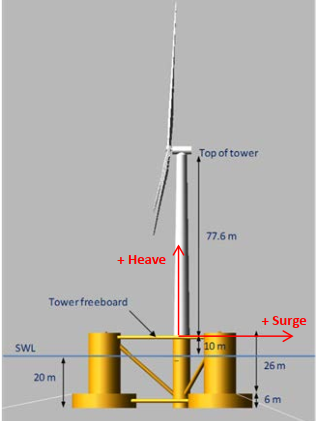
\includegraphics[width=0.99\textwidth]{OC4.png}
        \caption{\small OC4-DeepCwind floating wind system design. (Robertson et al., 2014)}
        \label{fig:OC4}
    \end{minipage}
    \hfill
    \begin{minipage}{0.5\textwidth}
        \centering
        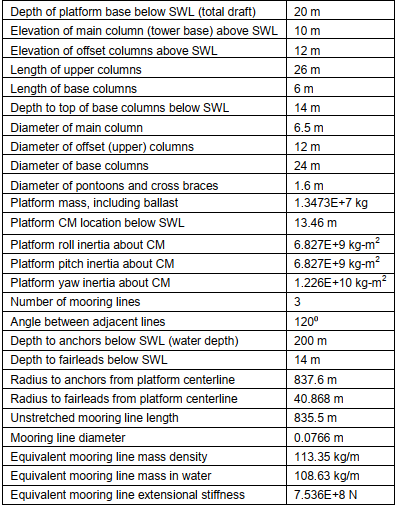
\includegraphics[width=0.97\textwidth]{characteristics.png}
        \caption{\small Summary of semisubmersible properties (Robertson et al., 2014)}
        \label{fig:characteristics}
    \end{minipage}
\end{figure}

\begin{table}[H]
    \centering
    \caption{Load cases run in OC4 Phase II. (Robertson et al., 2014)}
    \label{tab:image_table}
    \begin{tabular}{c}
        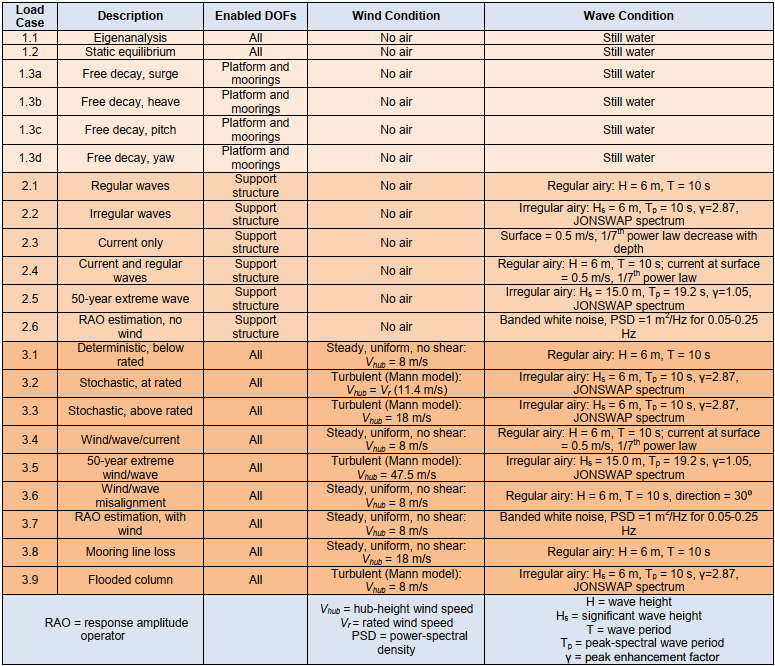
\includegraphics[width=1\textwidth]{table_3.png} \\
    \end{tabular}
\end{table}


\section{Pre-existing Model Analysis}

\hspace*{0.5cm}In this section, the analysis of the OC4 semisubmersible platform was conducted using a pre-existing model in OpenFAST called "5MW\_OC4Semi\_WSt\_WavesWN". The model was subjected to free decay and wave-induced load cases, namely Group 1.3X and 2.x, as outlined in the study by Robertson et al. (2014). The results were processed using BEMRosetta to extract natural frequencies and generate response graphs.

\subsection{Free Decay Tests}
\hspace*{0.5cm}The free decay tests involves subjecting the platform to initial displacements and allowing it to oscillate freely. Each of the four cases from 1.3a to 1.3d analyze the four individual degrees of freedom, specifically surge, heave, pitch, and yaw. The platform is given an initial displacement in the respective degree of freedom for each load case. The motion response of the platform was calculated using OpenFAST, and the natural frequencies were extracted from the time-domain data using the Fast Fourier Transform (FFT) method on BEMRosetta. The motion results of the 1.3a and 1.3b can be seen in Figures 3-14. The natural frequencies obtained from the tests for 6 degrees of freedom are shown in Figures 16-21 and consistent with the reference study, confirming the accuracy of the modeling approach \autoref{fig:nat_freq}.
\vspace{0.3cm}

%%1.3a figures
\begin{figure}[H]
    \begin{minipage}{0.48\textwidth}
        \centering
        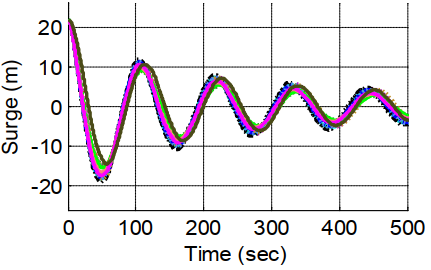
\includegraphics[width=0.97\textwidth]{1.3a_surge.png}
        \caption{\small Surge free decay platform motion response for 1.3a (Robertson et al., 2014)}
        \label{fig:1.3a_surge}
    \end{minipage}
    \hfill
    \begin{minipage}{0.49\textwidth}
        \centering
        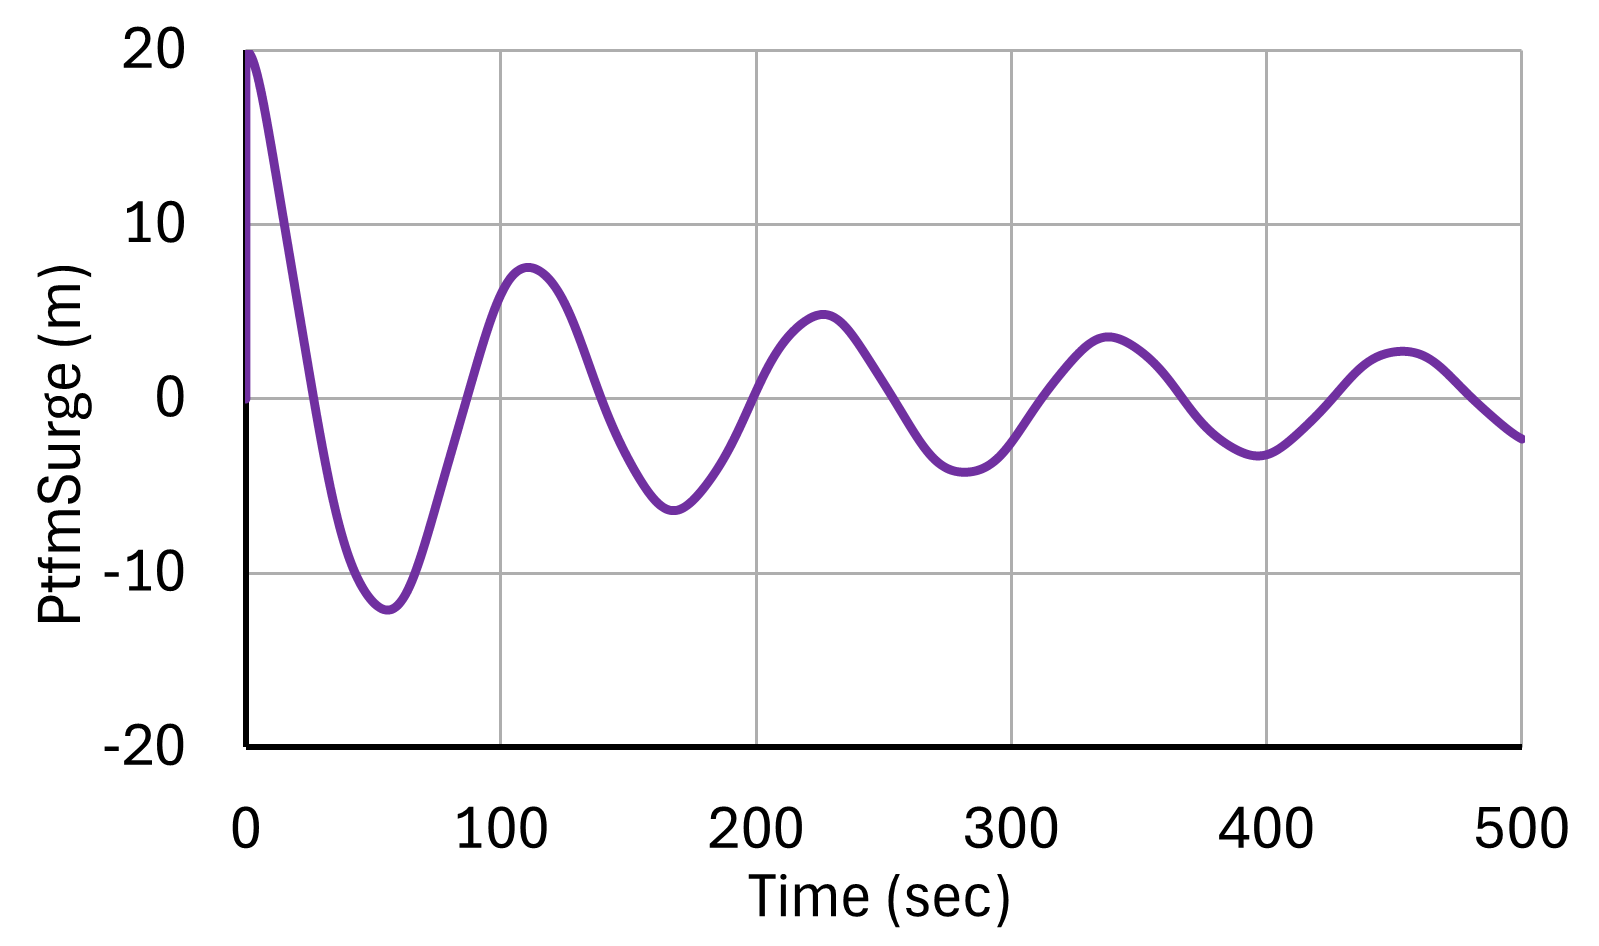
\includegraphics[width=1\textwidth]{1.3a_surge_mine.png}
        \caption{\small Surge free decay platform motion response for 1.3a}
        \label{fig:1.3a_surge_mine}
    \end{minipage}
\end{figure}

\begin{figure}[H]
    \begin{minipage}{0.48\textwidth}
        \centering
        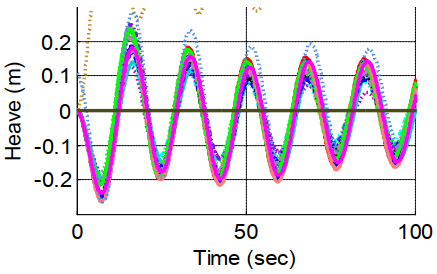
\includegraphics[width=0.97\textwidth]{1.3a_heave.png}
        \caption{\small Heave free decay platform motion response for 1.3a (Robertson et al., 2014)}
        \label{fig:1.3a_heave}
    \end{minipage}
    \hfill
    \begin{minipage}{0.49\textwidth}
        \centering
        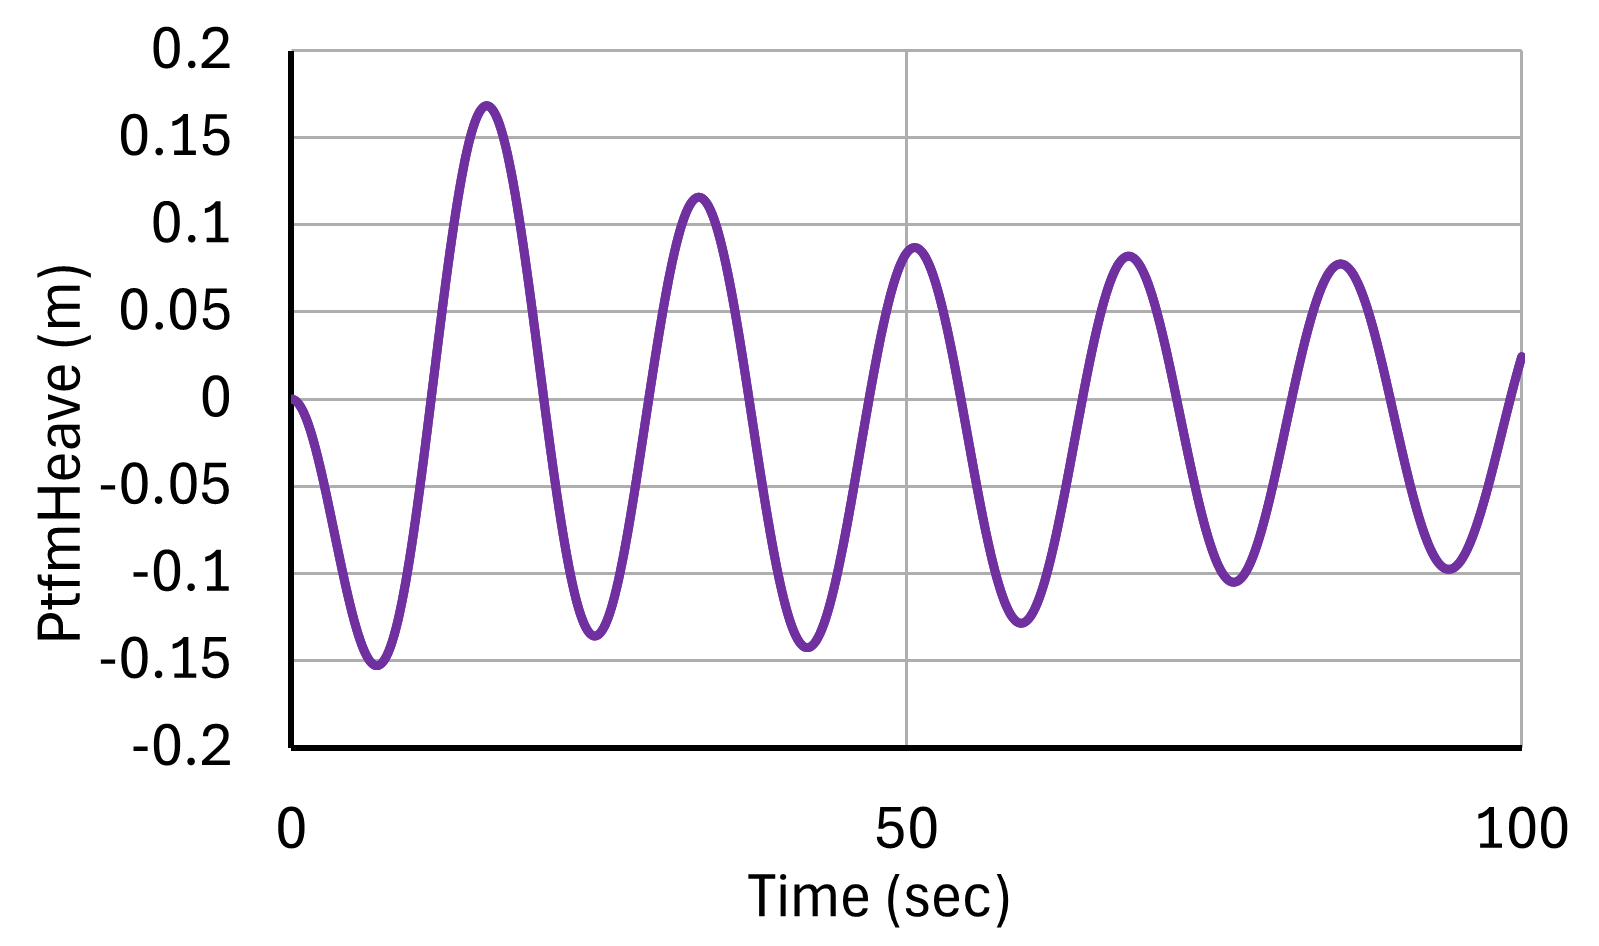
\includegraphics[width=1\textwidth]{1.3a_heave_mine.png}
        \caption{\small Heave free decay platform motion response for 1.3a}
        \label{fig:1.3a_heave_mine}
    \end{minipage}
\end{figure}

\begin{figure}[H]
    \begin{minipage}{0.48\textwidth}
        \centering
        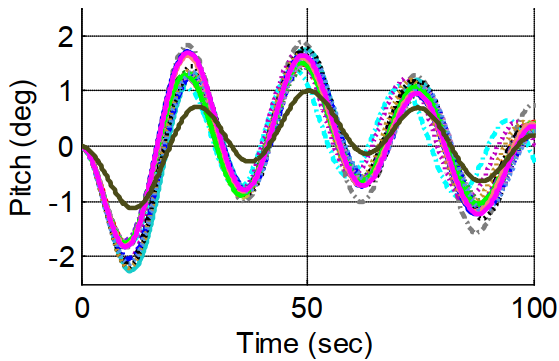
\includegraphics[width=0.97\textwidth]{1.3a_pitch.png}
        \caption{\small Pitch free decay platform motion response for 1.3a (Robertson et al., 2014)}
        \label{fig:1.3a_pitch}
    \end{minipage}
    \hfill
    \begin{minipage}{0.49\textwidth}
        \centering
        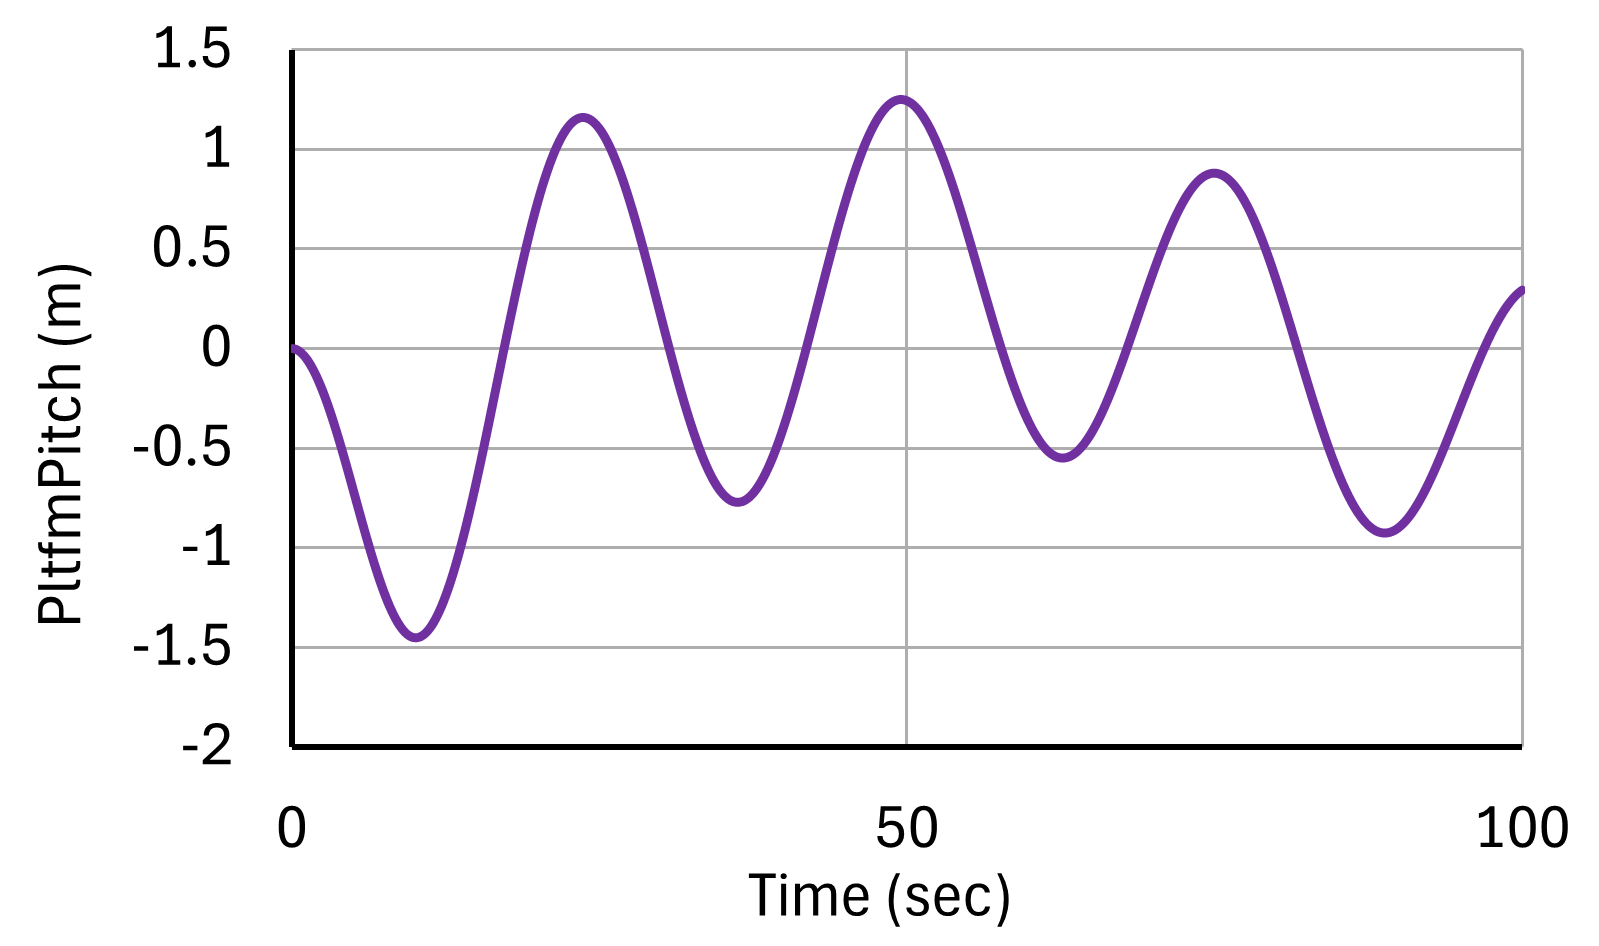
\includegraphics[width=1\textwidth]{1.3a_pitch_mine.png}
        \caption{\small Pitch free decay platform motion response for 1.3a}
        \label{fig:1.3a_pitch_mine}
    \end{minipage}
\end{figure}

%%1.3b figures
\begin{figure}[H]
    \begin{minipage}{0.47\textwidth}
        \centering
        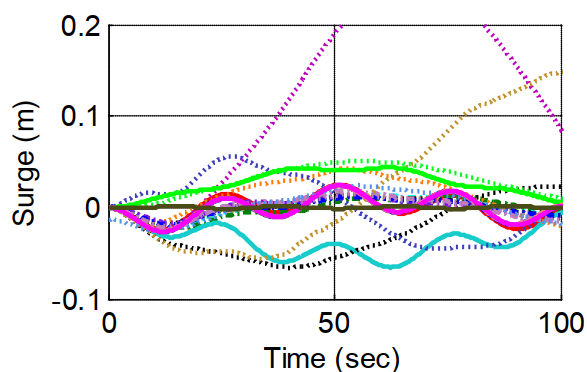
\includegraphics[width=0.97\textwidth]{1.3b_surge.png}
        \caption{\small Surge free decay platform motion response for 1.3b (Robertson et al., 2014)}
        \label{fig:1.3b_surge}
    \end{minipage}
    \hfill
    \begin{minipage}{0.5\textwidth}
        \centering
        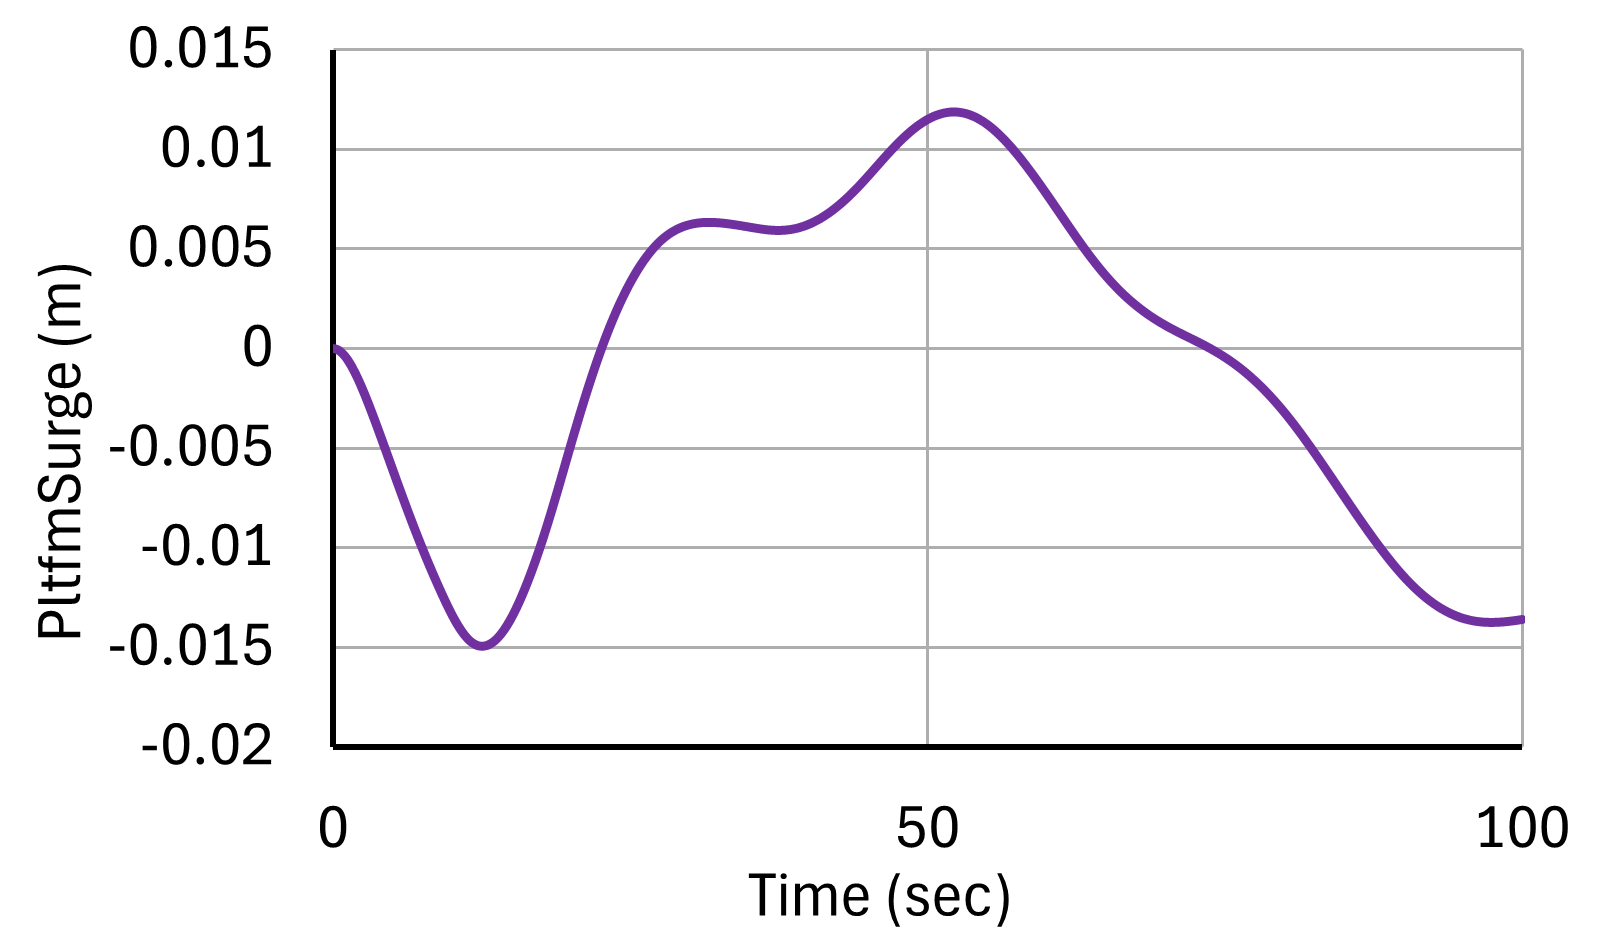
\includegraphics[width=1\textwidth]{1.3b_surge_mine.png}
        \caption{\small Surge free decay platform motion response for 1.3b}
        \label{fig:1.3b_surge_mine}
    \end{minipage}
\end{figure}

\begin{figure}[H]
    \begin{minipage}{0.47\textwidth}
        \centering
        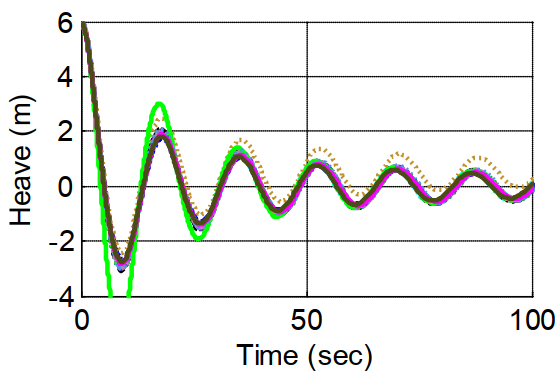
\includegraphics[width=0.97\textwidth]{1.3b_heave.png}
        \caption{\small Heave free decay platform motion response for 1.3b (Robertson et al., 2014)}
        \label{fig:1.3b_heave}
    \end{minipage}
    \hfill
    \begin{minipage}{0.5\textwidth}
        \centering
        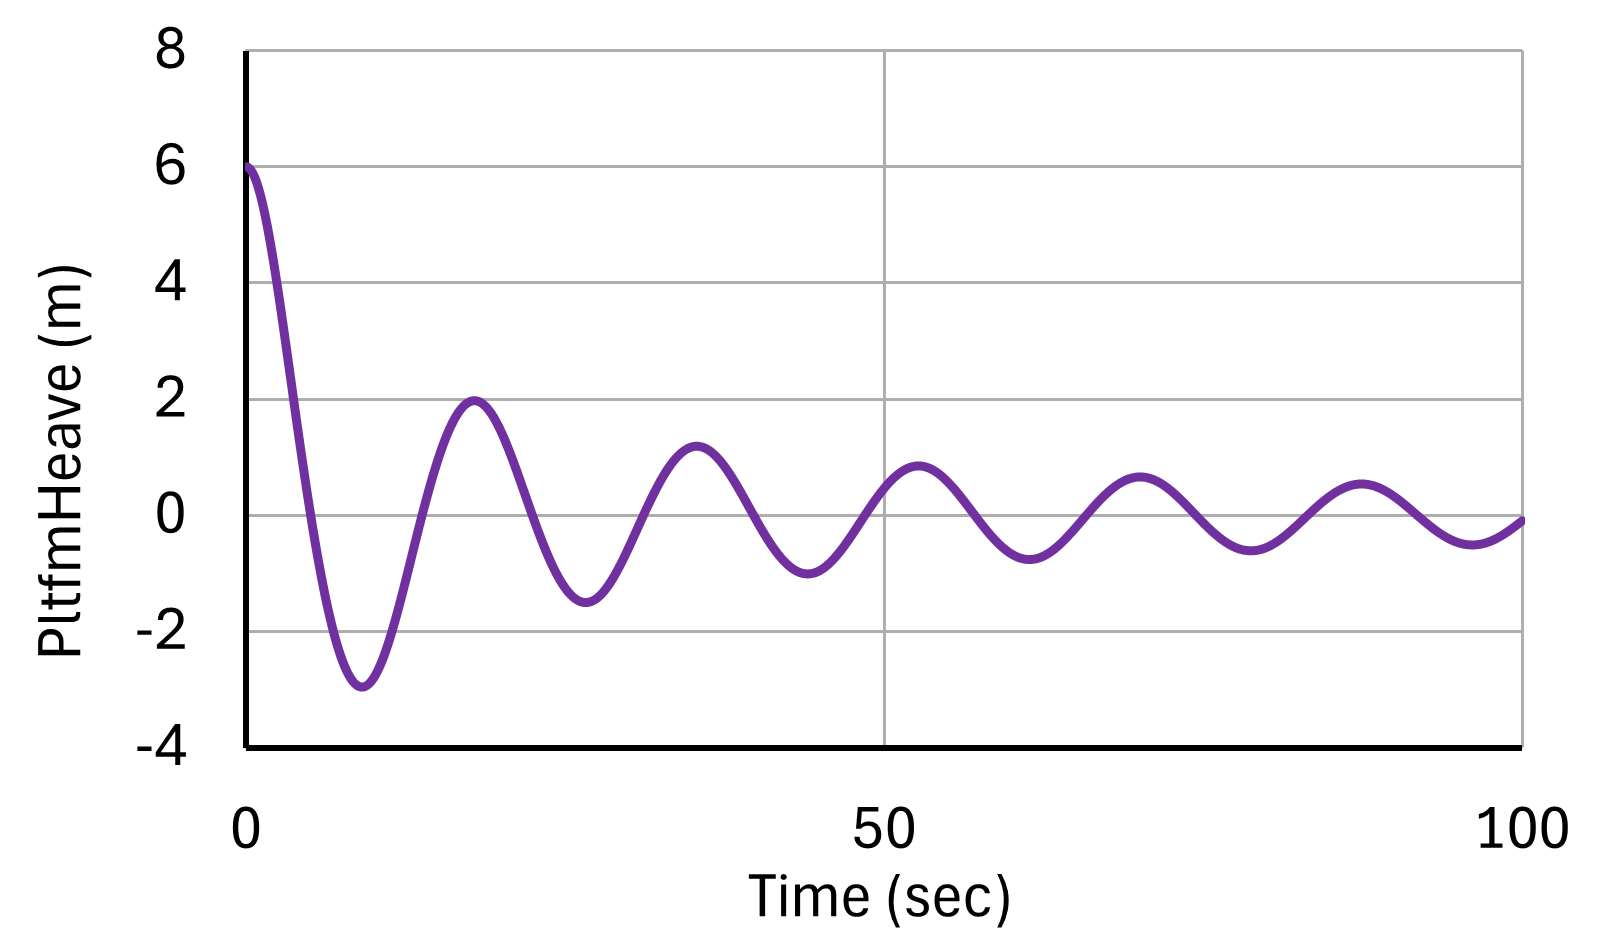
\includegraphics[width=1\textwidth]{1.3b_heave_mine.png}
        \caption{\small Heave free decay platform motion response for 1.3b}
        \label{fig:1.3b_heave_mine}
    \end{minipage}
\end{figure}

\begin{figure}[H]
    \begin{minipage}{0.47\textwidth}
        \centering
        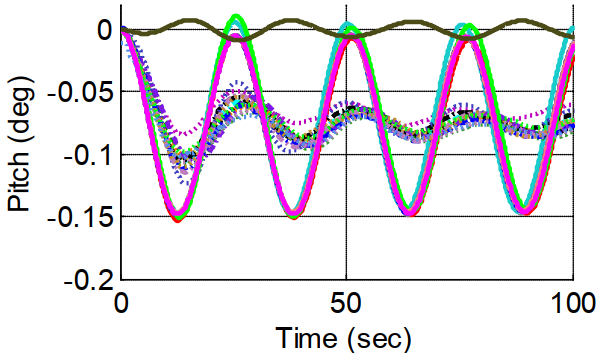
\includegraphics[width=0.97\textwidth]{1.3b_pitch.png}
        \caption{\small Pitch free decay platform motion response for 1.3b (Robertson et al., 2014)}
        \label{fig:1.3b_pitch}
    \end{minipage}
    \hfill
    \begin{minipage}{0.5\textwidth}
        \centering
        \vspace{-0.3cm}
        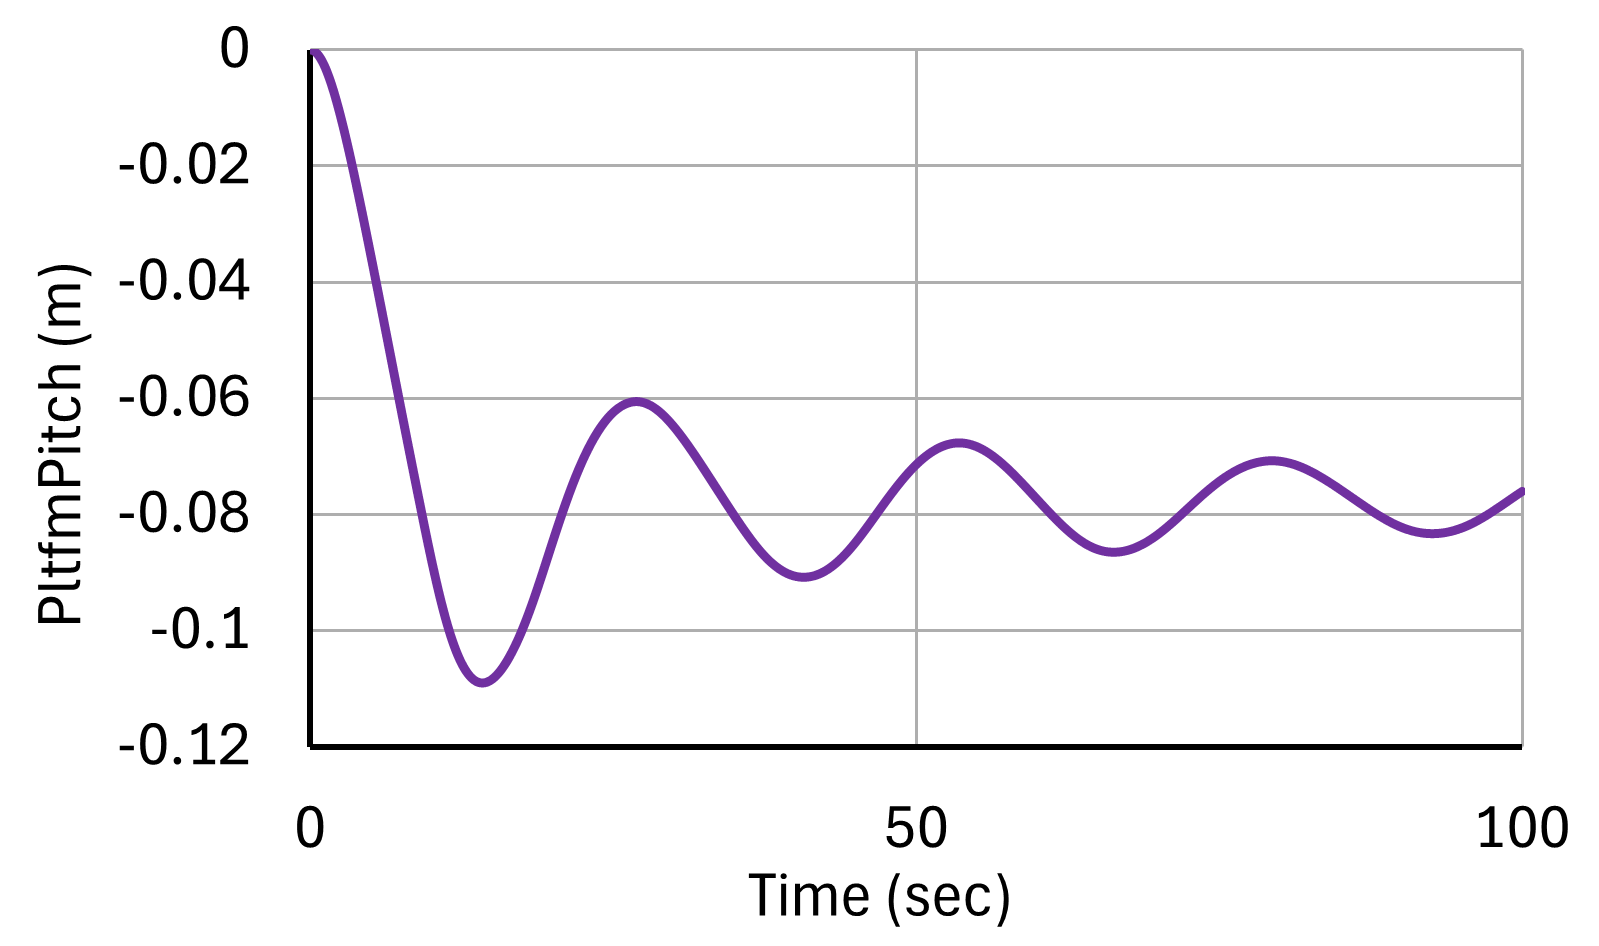
\includegraphics[width=1\textwidth]{1.3b_pitch_mine.png}
        \caption{\small Pitch free decay platform motion response for 1.3b}
        \label{fig:1.3b_pitch_mine}
    \end{minipage}
\end{figure}

When the graphs plotted for the surge, heave, and pitch motions are compared to the reference study, it is observed that the results are consistent in terms of the overall pattern of the motion response. Specifically, for the 1.3b case, the pitch motion response shows a very close resemblance to the distinct grouping using Morison’s equation for calculating the viscous drag (dotted or dash-dotted results) versus those using a quadratic drag matrix (solid line results).

%%natural frequencies

\begin{figure}[H]
    \centering
    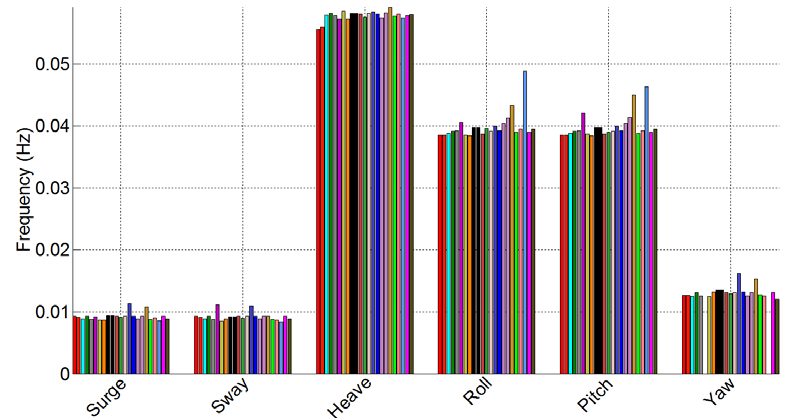
\includegraphics[width=0.9\textwidth]{nat_freq.png}
    \caption{\small Full-system natural frequencies (Robertson et al., 2014)}
    \label{fig:nat_freq}
\end{figure}

\begin{figure}[H]
    \begin{minipage}{0.49\textwidth}
        \centering
        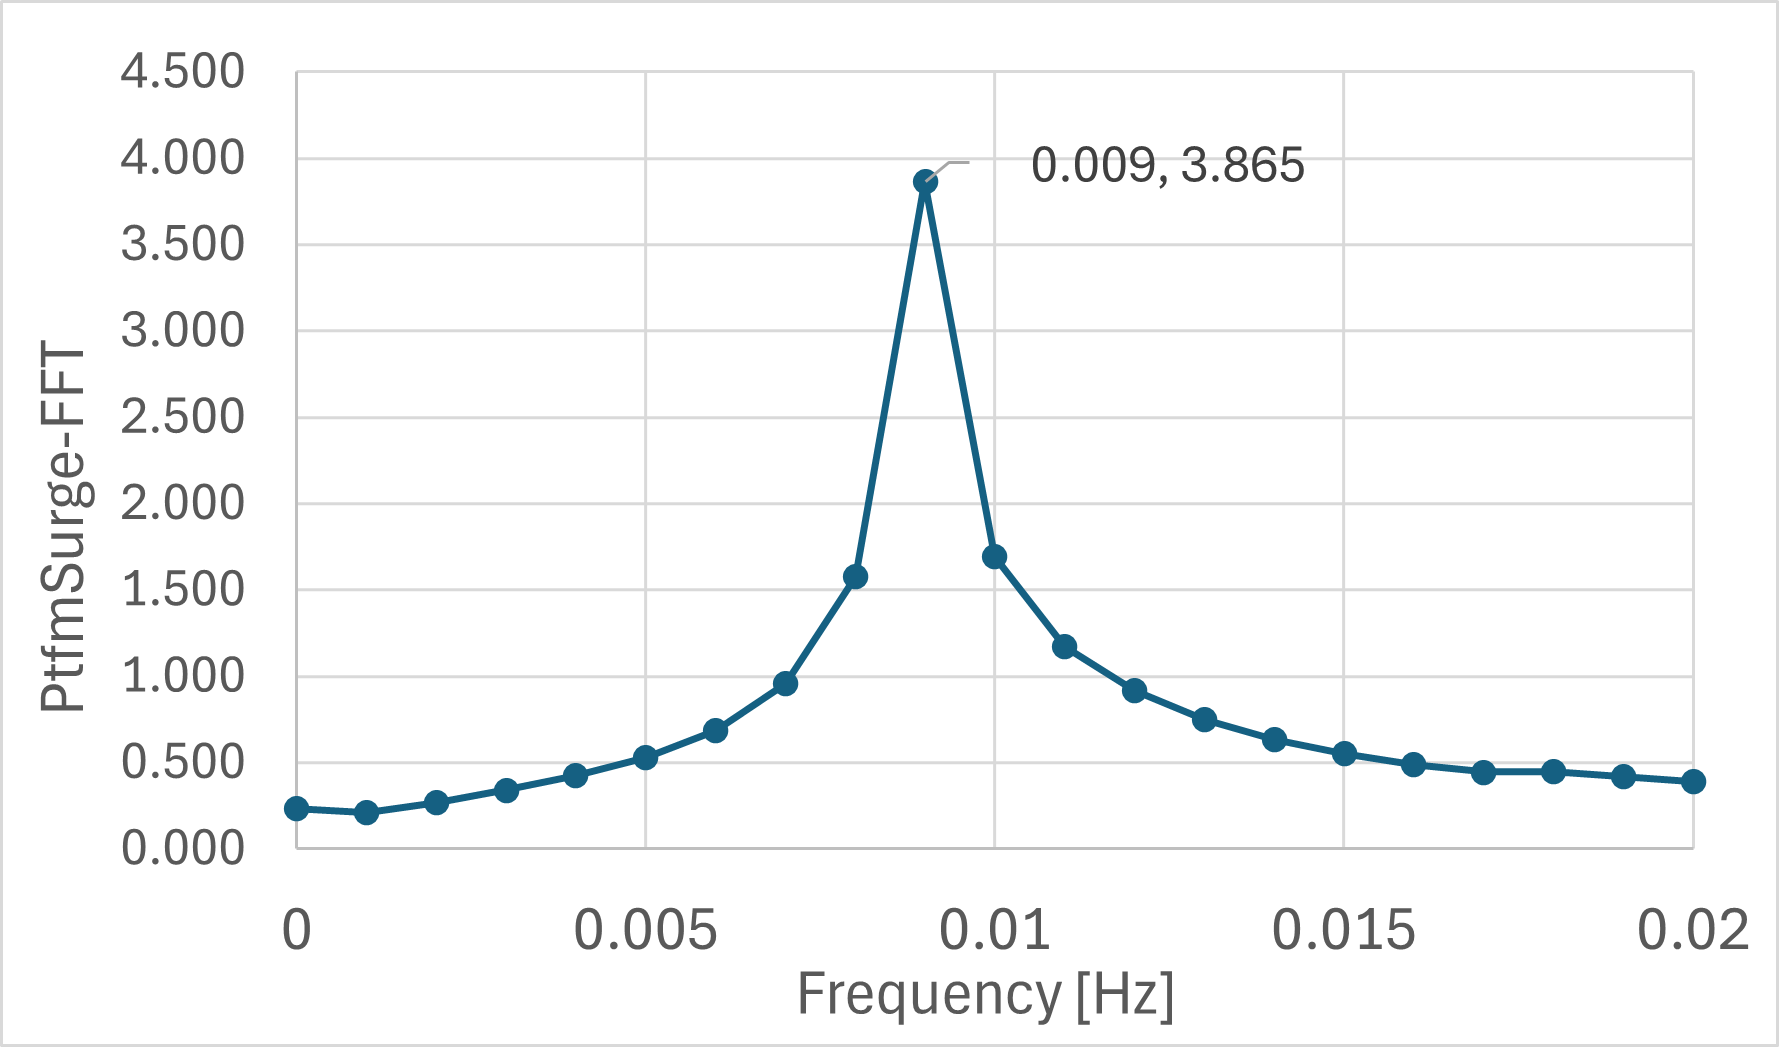
\includegraphics[width=1\textwidth]{nat_freq_surge.png}
        \caption{\small Surge natural frequency}
        \label{fig:nat_freq_surge}
    \end{minipage}
    \hfill
    \begin{minipage}{0.5\textwidth}
        \centering
        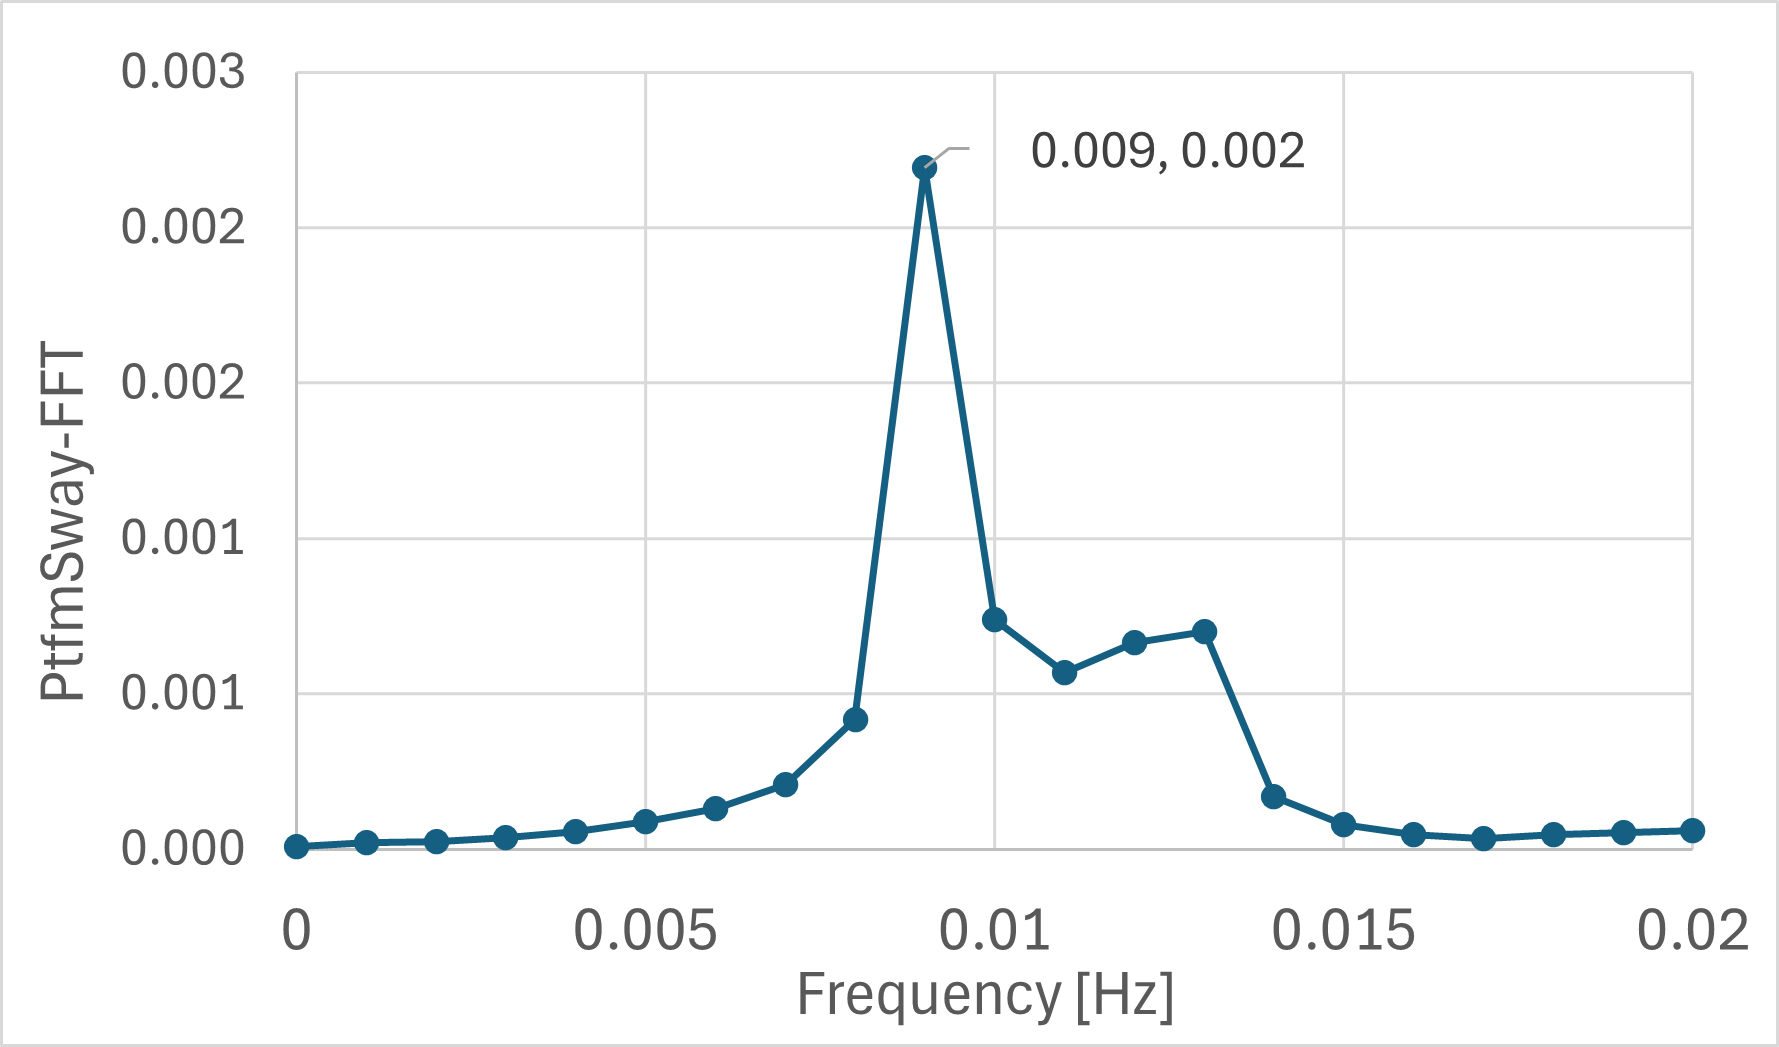
\includegraphics[width=1\textwidth]{nat_freq_sway.png}
        \caption{\small Sway natural frequency}
        \label{fig:nat_freq_sway}
    \end{minipage}
\end{figure}

\begin{figure}[H]
    \begin{minipage}{0.49\textwidth}
        \centering
        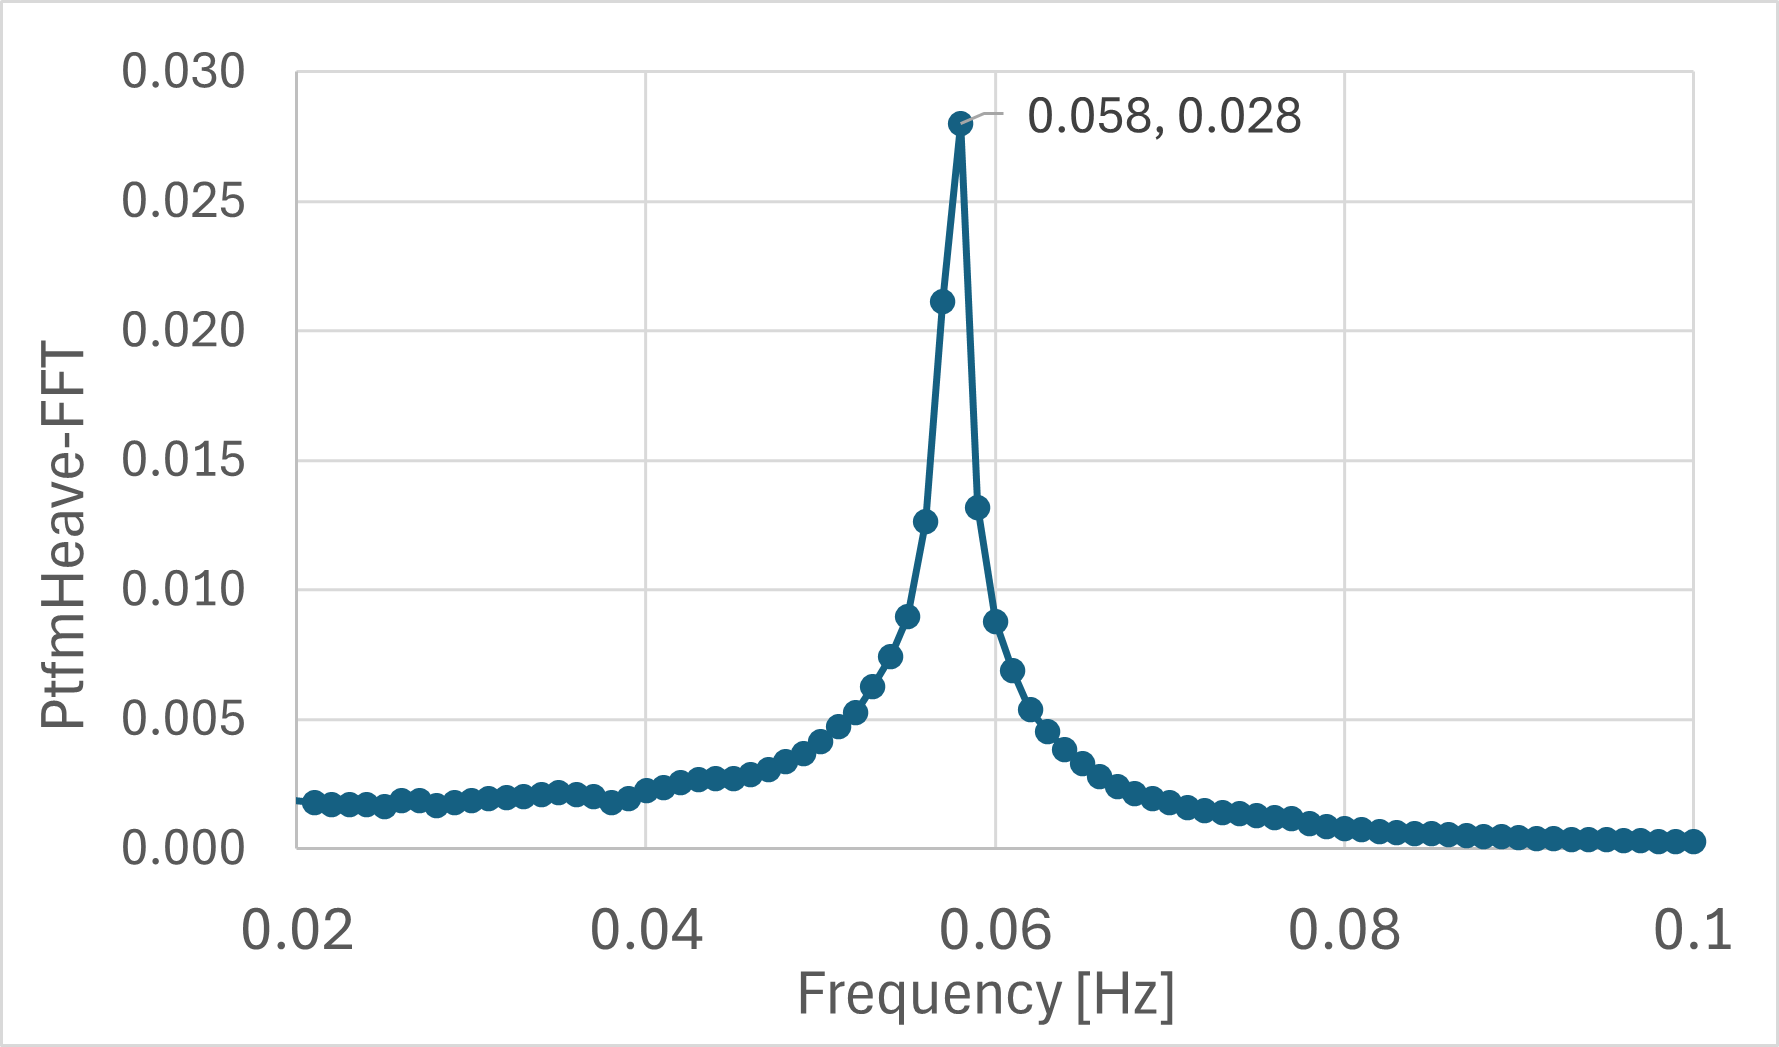
\includegraphics[width=1\textwidth]{nat_freq_heave.png}
        \caption{\small Heave natural frequency}
        \label{fig:nat_freq_heave}
    \end{minipage}
    \hfill
    \begin{minipage}{0.5\textwidth}
        \centering
        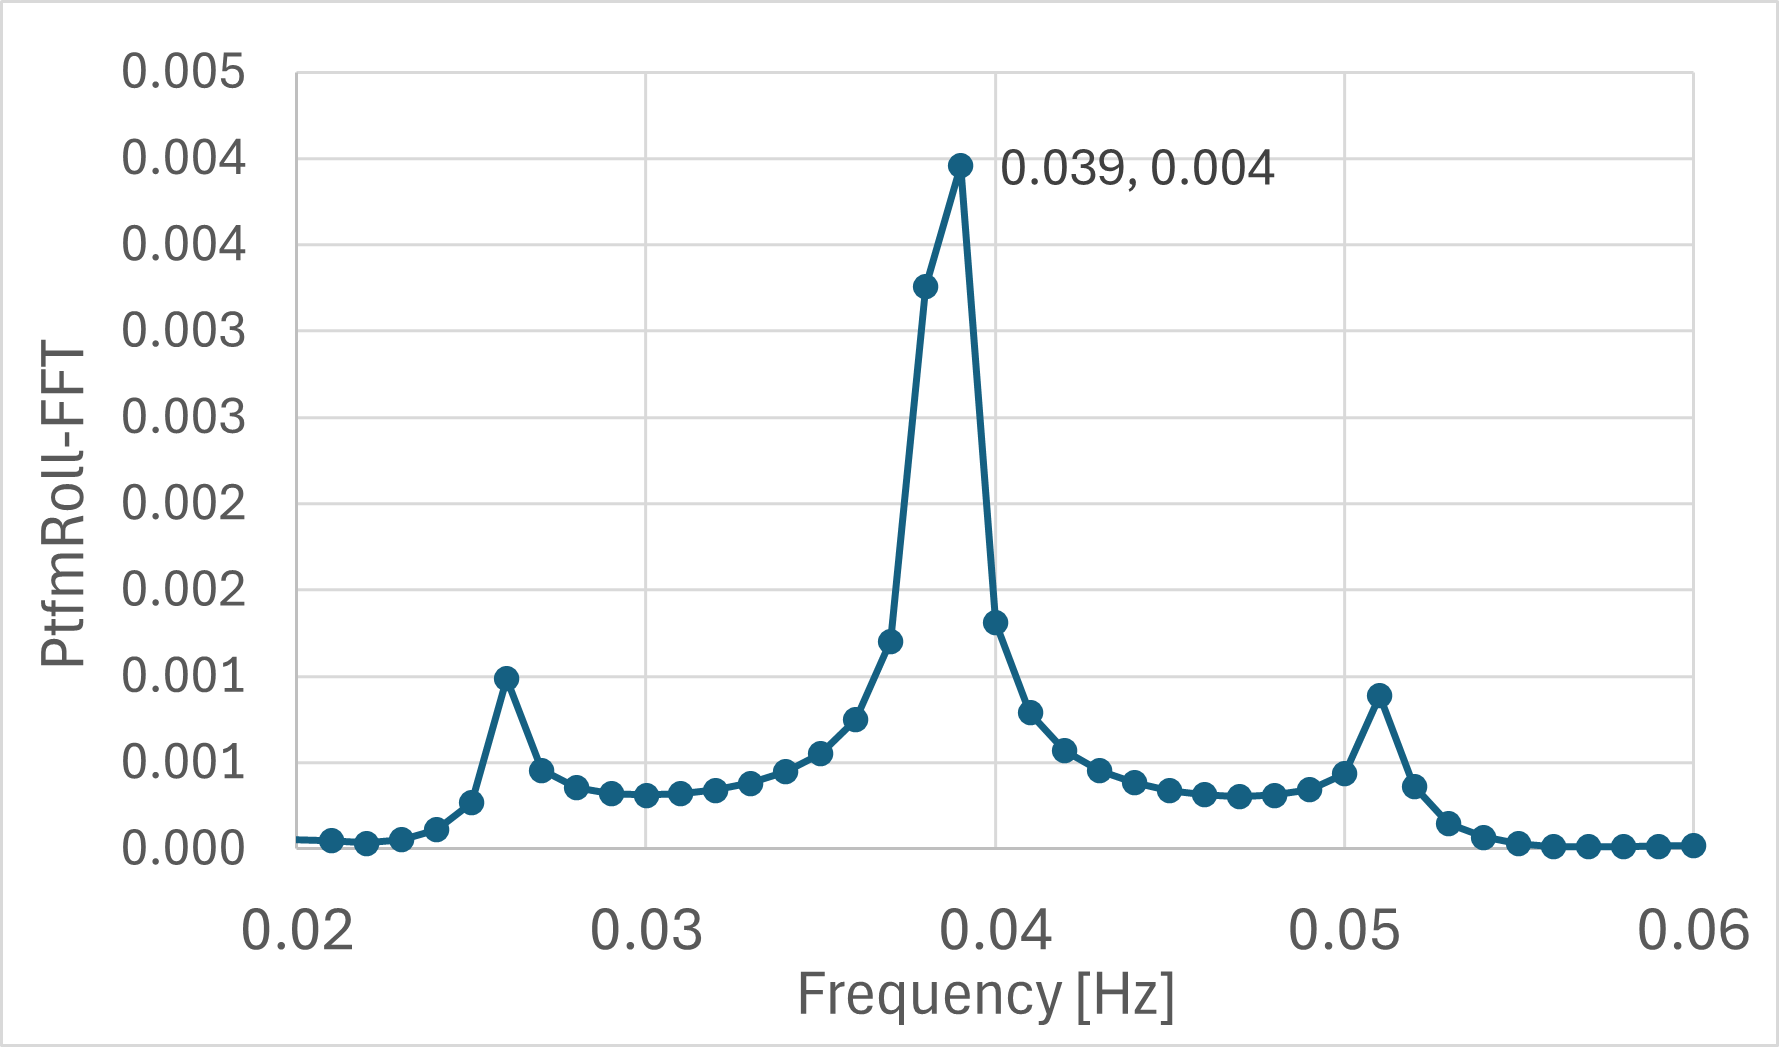
\includegraphics[width=1\textwidth]{nat_freq_roll.png}
        \caption{\small Roll natural frequency}
        \label{fig:nat_freq_roll}
    \end{minipage}
\end{figure}

\begin{figure}[H]
    \begin{minipage}{0.49\textwidth}
        \centering
        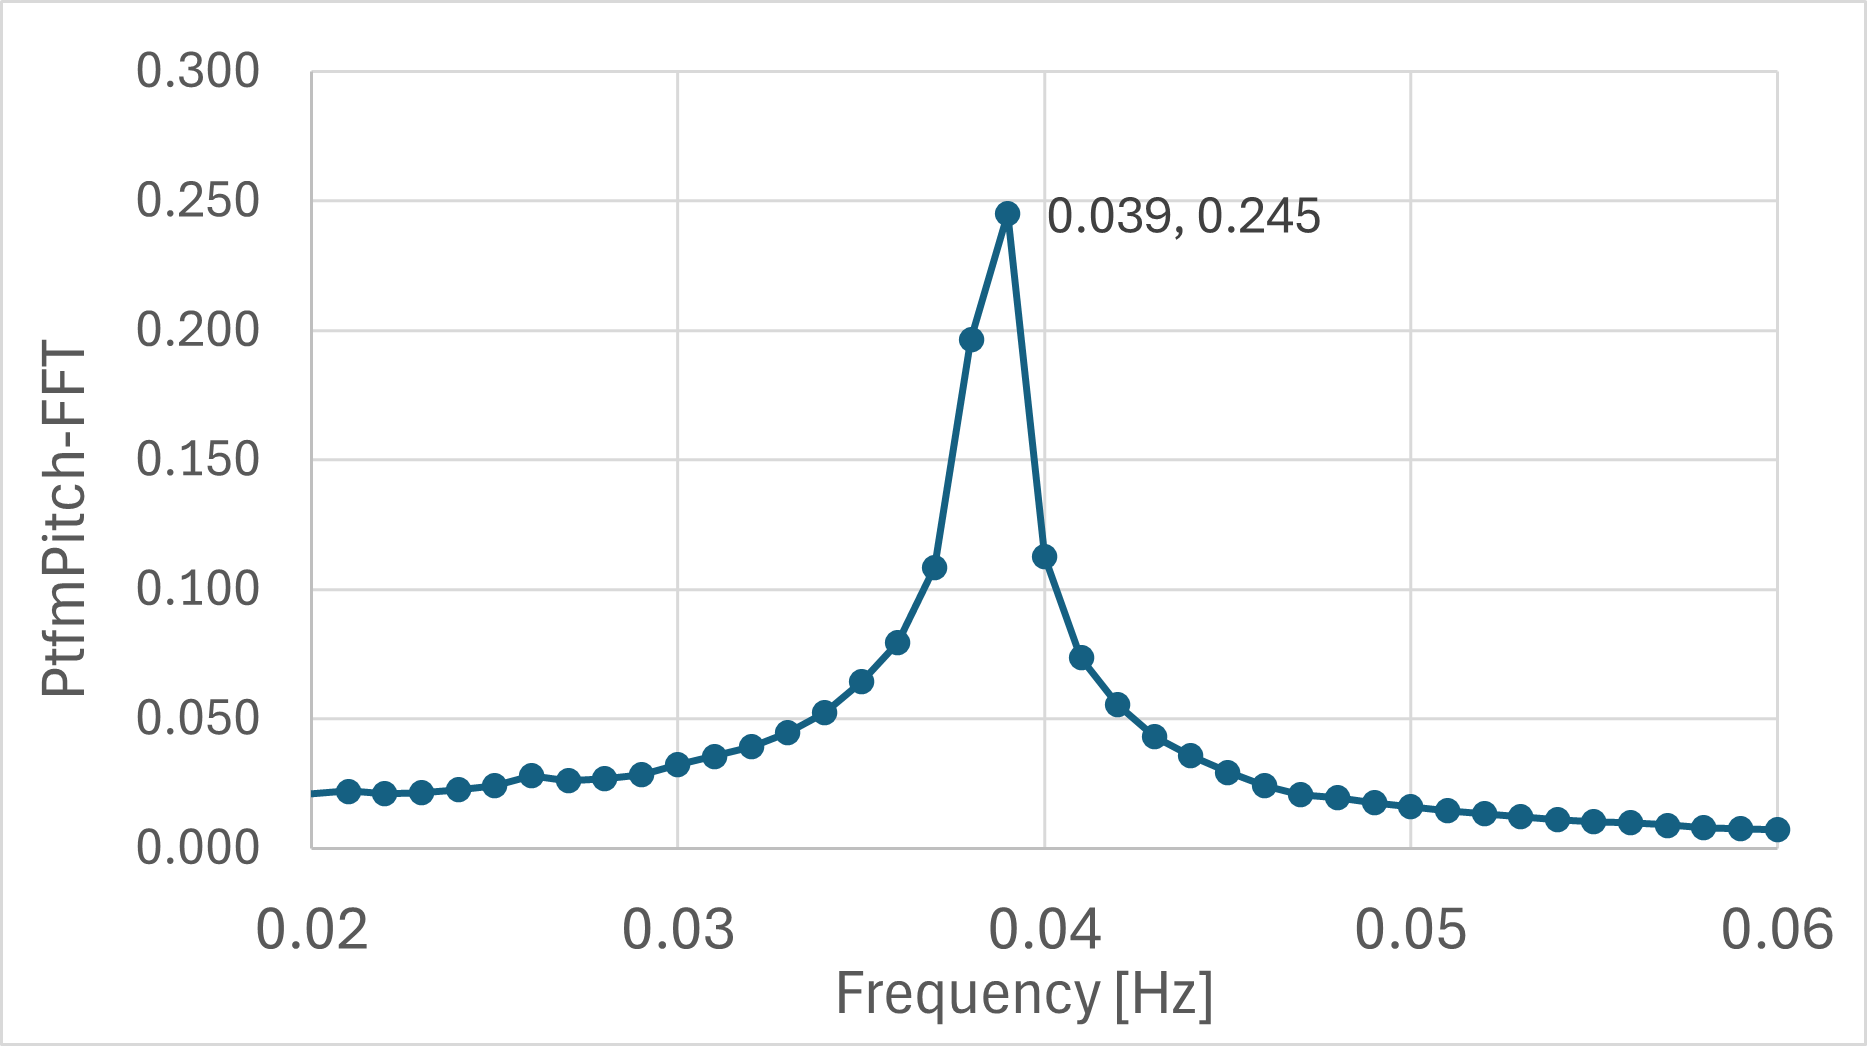
\includegraphics[width=1\textwidth]{nat_freq_pitch.png}
        \caption{\small Pitch natural frequency}
        \label{fig:nat_freq_pitch}
    \end{minipage}
    \hfill
    \begin{minipage}{0.5\textwidth}
        \centering
        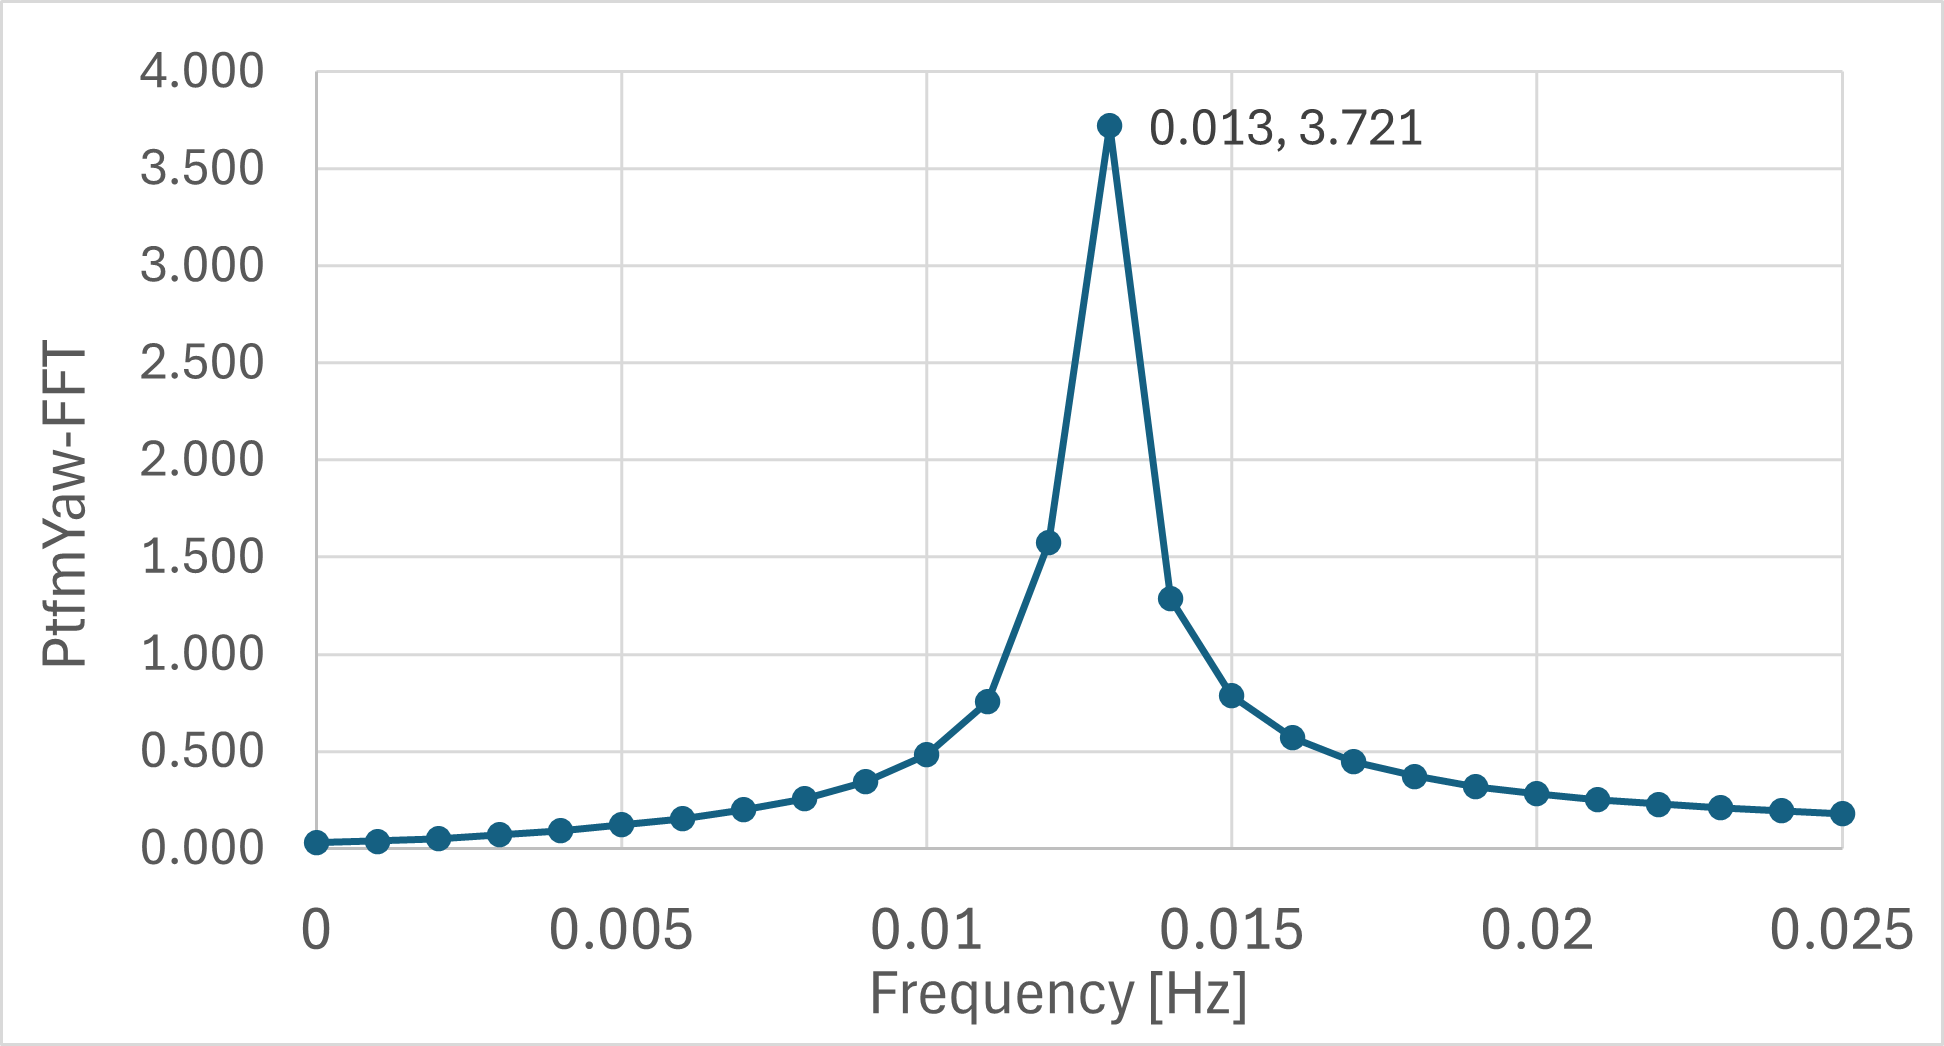
\includegraphics[width=1\textwidth]{nat_freq_yaw.png}
        \caption{\small Yaw natural frequency}
        \label{fig:nat_freq_yaw}
    \end{minipage}
\end{figure}

The natural frequency analysis of the semisubmersible platform shows a distinction in the magnitude of these frequencies across the six degrees of freedom. Specifically, the natural frequencies for heave, roll and pitch were notably higher than those for surge, sway and yaw, with heave demonstrating highest frequency overall.

This difference originates from the restoring mechanisms associated with each degree of freedom. Heave, roll, and pitch are governed by strong hydrostatic restoring forces. For heave, this is primarily due to buoyancy, where vertical displacements lead to significant changes in the buoyant force. Roll and pitch experience restoring moments due to the platform's metacentric heights, which resist angular displacements. These restoring forces result in higher natural frequencies. In contrast, the restoring forces for surge and sway are minimal for small displacements, leading to very low natural frequencies. The yaw response shows restoring strength of similar but reduced magnitude to roll and pitch. This rotational stiffness is primarily from hydrodynamic sources like the geometry of the body, rather than the hydrostatic mechanisms that dominate roll and pitch (Jonkman, 2007).


\subsection{Wave and Current Induced Tests}
\hspace*{0.5cm}The wave-induced responses were analyzed by applying regular and irregular waves to the platform. The peak period of the waves were taken as 10 seconds, and the significant wave height was set to 6 meters. For the irregular waves, the JONSWAP spectrum was used to generate the wave field, with a peak wave shape parameter of 2.87. 


\subsubsection{Load Case 2.1}

\hspace{0.5cm}Load case 2.1 was used to analyze the platform’s response to regular waves, focusing on heave, pitch, surge motions, and the tension force at fairlead 2. The analysis was conducted using two approaches: one incorporating second-order drift effects through quadratic transfer functions (QTF) to account for low-frequency wave forces, and another excluding drift effects to isolate first-order wave responses. The results, processed using BEMRosetta, were compared to the reference study (Figures 22–29).

The platform's motion responses showed a strong resemblence to NREL's FAST v8 simulations when drift effects were neglected, as expected, since they did not utilize QTF-based second-order analysis in their calculations. This alignment confirms that both approaches produced equivalent first-order hydrodynamic responses. This consistency validates the first-order hydrodynamic modeling approach. However, when drift forces were introduced, surge motion showed significant sensitivity to QTF inclusion due to its weak hydrodynamic restoring forces. In contrast, heave and pitch motions remained relatively unaffected by second-order effects because of their strong hydrostatic stiffness and higher natural frequencies (Figures 16, 18, and 20) make them more responsive to first-order wave excitations. The observed reduction in maximum fairlead 2 tension when neglecting QTF stems from this mooring point's direct coupling with surge motion along the y-axis; as the slow-drift components were removed, both surge displacement and consequent line tension decreased proportionally. These tension results aligned with dynamic mooring models, validating that the simulation properly accounted for the mooring system's mass, stiffness, and damping characteristics.

%% 2.1 figures
\begin{figure}[H]
    \begin{minipage}{0.48\textwidth}
        \centering
        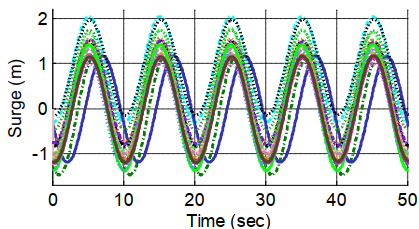
\includegraphics[width=1\textwidth]{2.1_surge.png}
        \caption{\small Surge response for 2.1 (Robertson et al., 2014)}
        \label{fig:2.1_surge}
    \end{minipage}
    \hfill
    \begin{minipage}{0.51\textwidth}
        \centering
        \vspace{-0.3cm}
        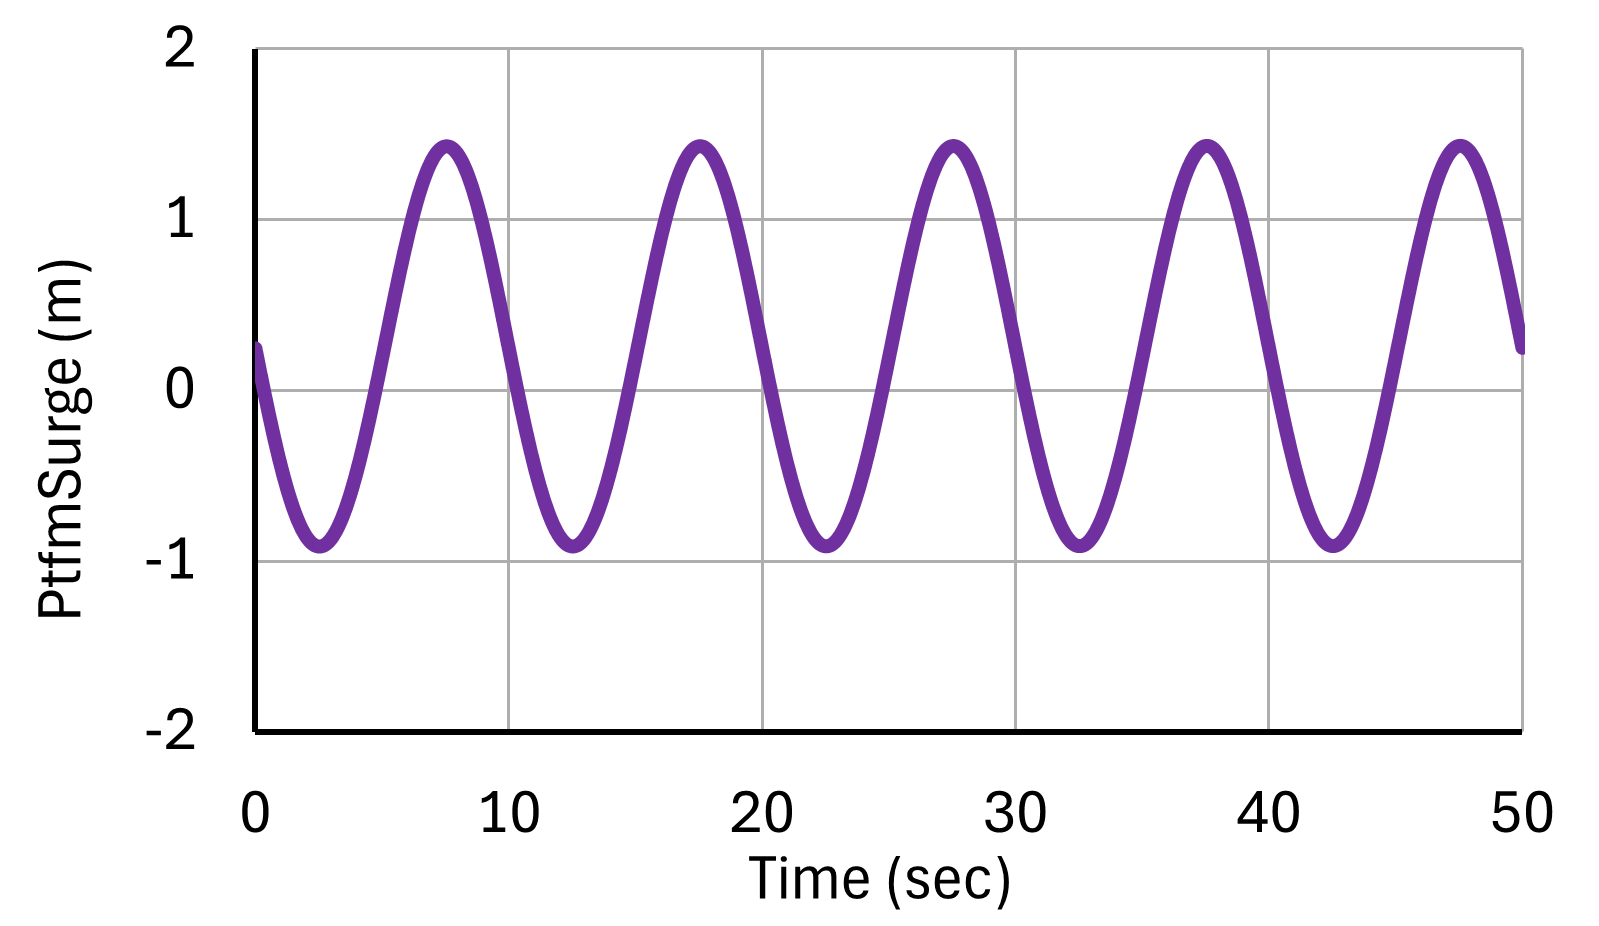
\includegraphics[width=1\textwidth]{2.1_surge_mine.png}
        \caption{\small Surge response for 2.1}
        \label{fig:2.1_surge_mine}
    \end{minipage}
\end{figure}

\begin{figure}[H]
    \begin{minipage}{0.48\textwidth}
        \centering
        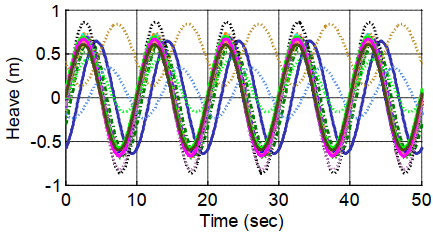
\includegraphics[width=1\textwidth]{2.1_heave.png}
        \caption{\small Heave response for 2.1 (Robertson et al., 2014)}
        \label{fig:2.1_heave}
    \end{minipage}
    \hfill
    \begin{minipage}{0.51\textwidth}
        \centering
        \vspace{-0.3cm}
        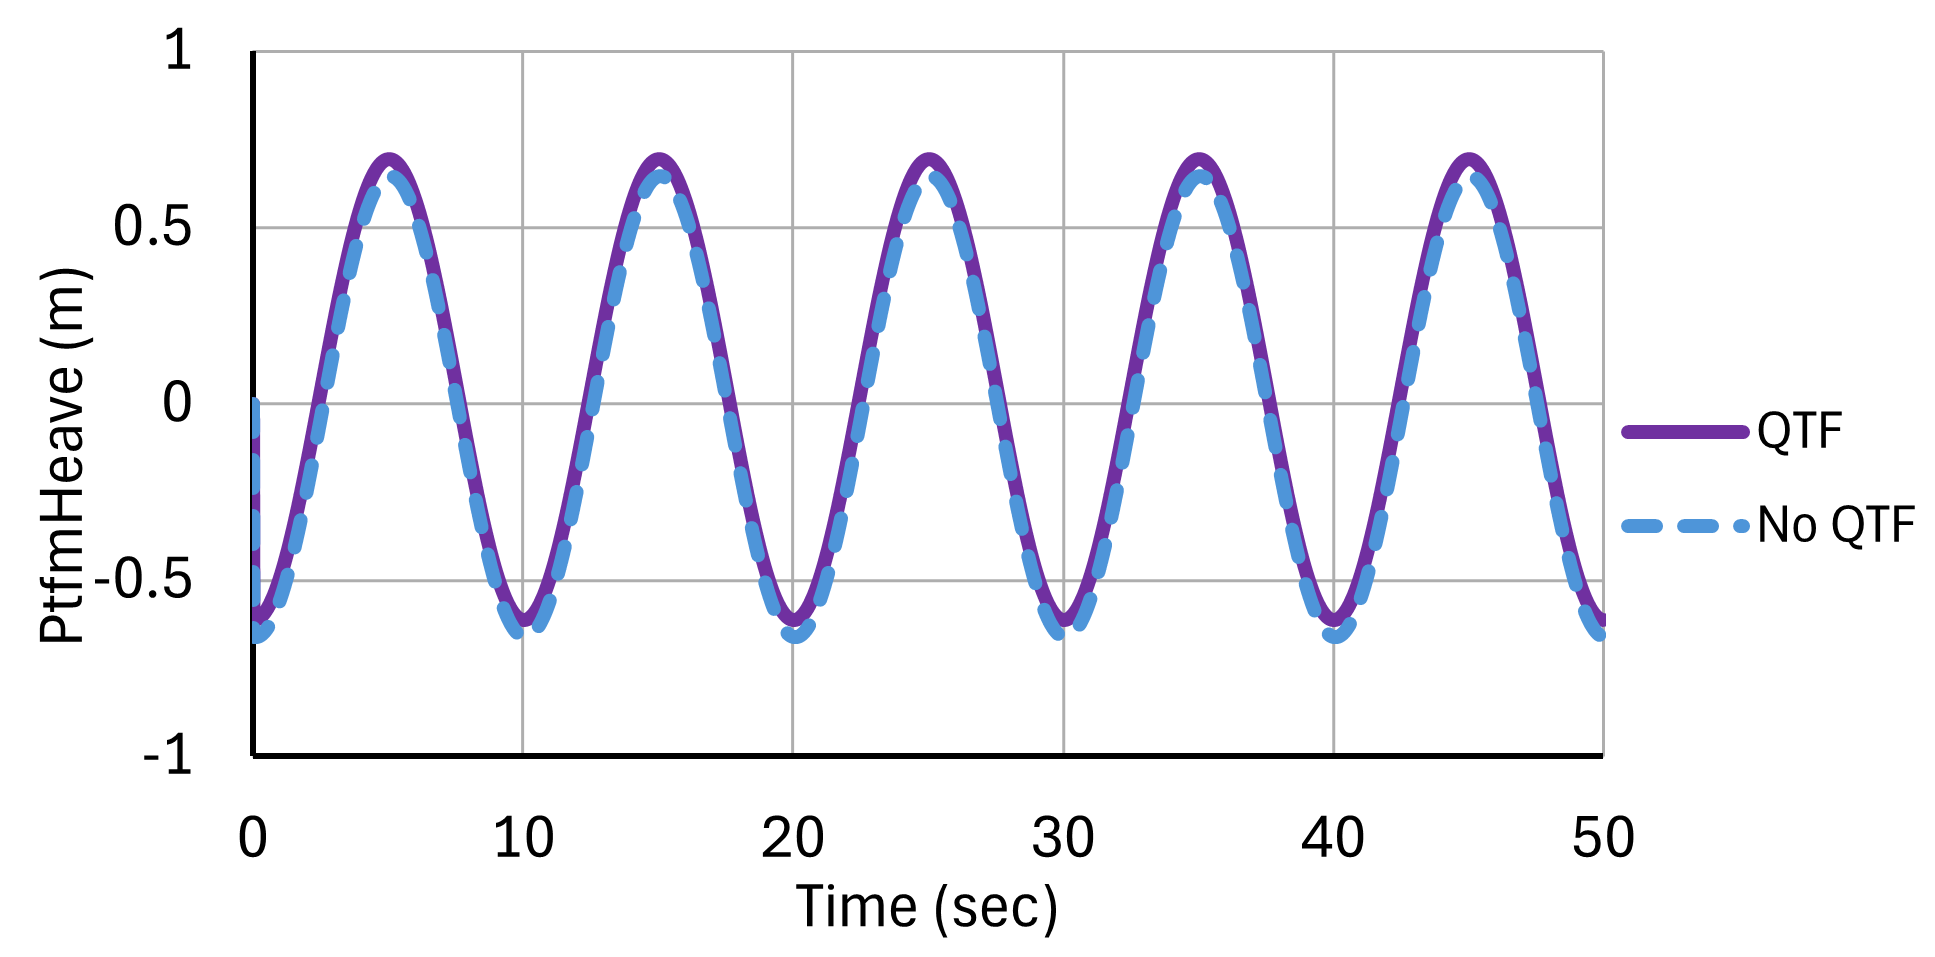
\includegraphics[width=1\textwidth]{2.1_heave_mine.png}
        \caption{\small Heave response for 2.1}
        \label{fig:2.1_heave_mine}
    \end{minipage}
\end{figure}

\begin{figure}[H]
    \begin{minipage}{0.48\textwidth}
        \centering
        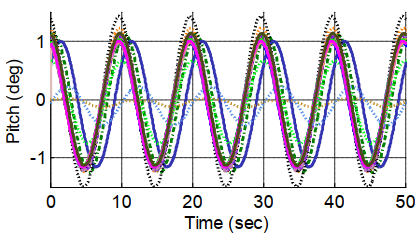
\includegraphics[width=1\textwidth]{2.1_pitch.png}
        \caption{\small Pitch response for 2.1 (Robertson et al., 2014)}
        \label{fig:2.1_pitch}
    \end{minipage}
    \hfill
    \begin{minipage}{0.51\textwidth}
        \centering
        \vspace{-0.3cm}
        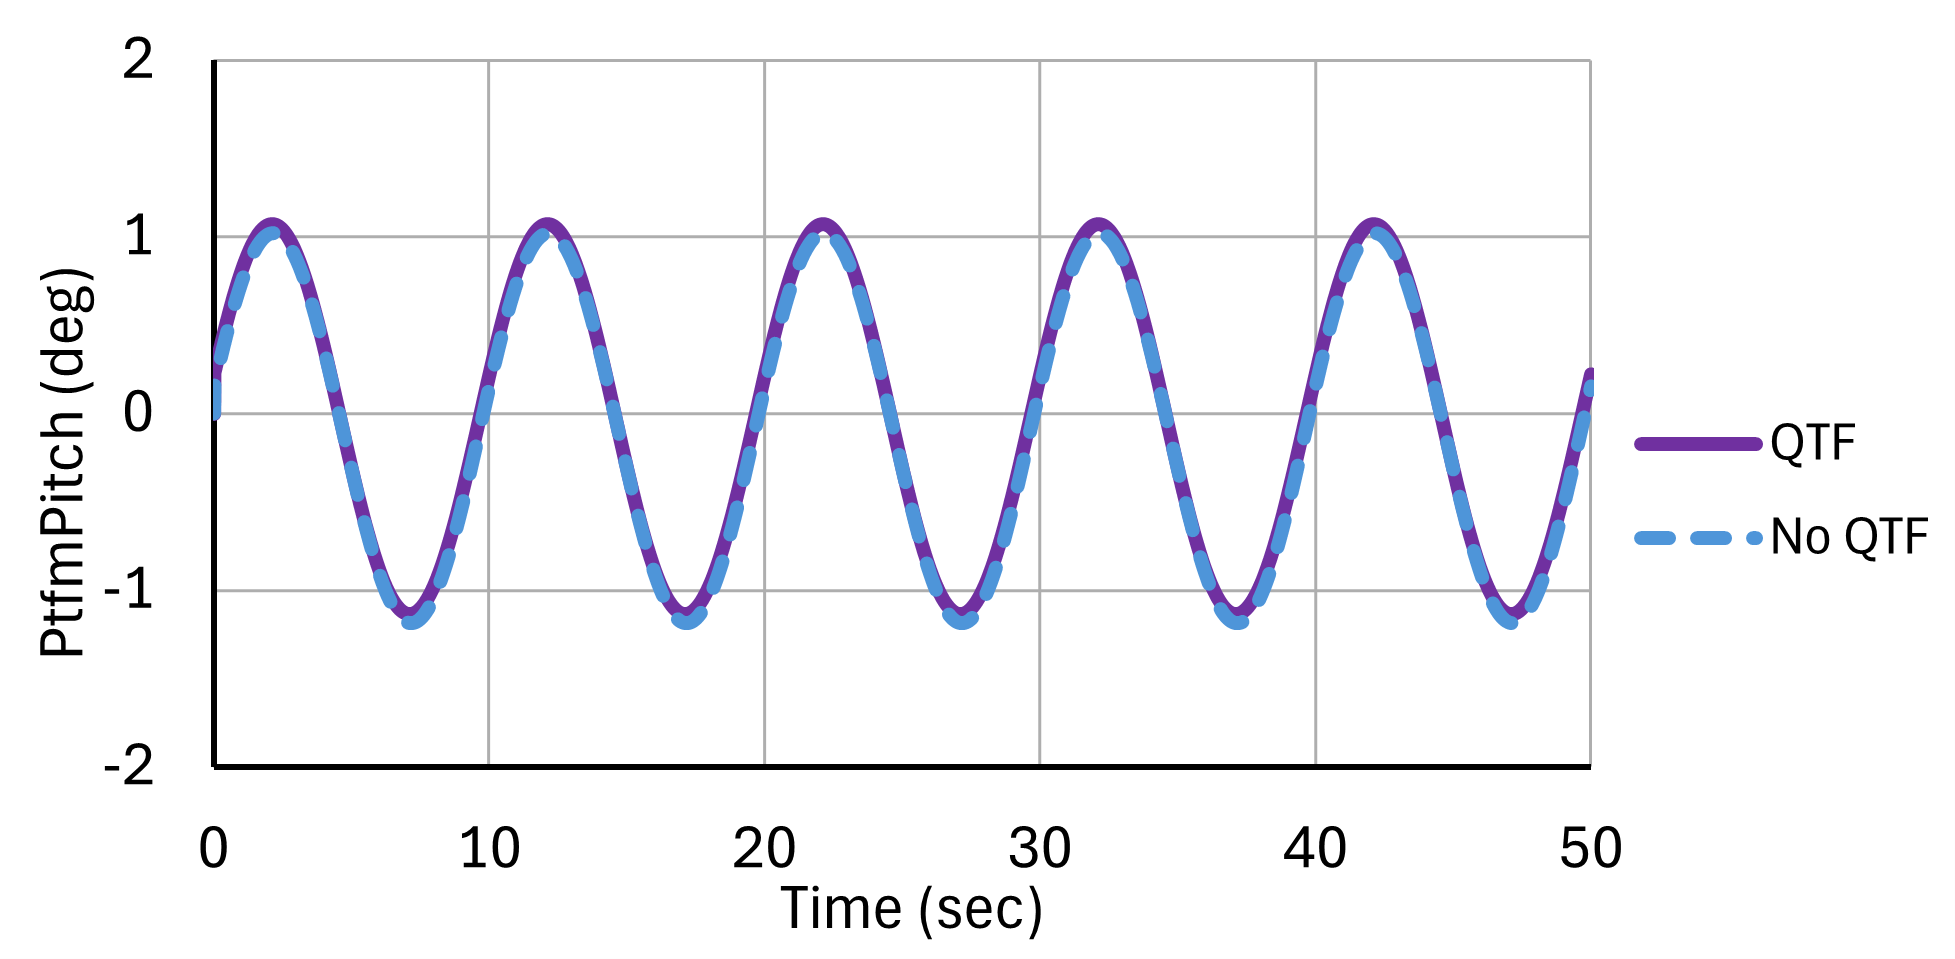
\includegraphics[width=1\textwidth]{2.1_pitch_mine.png}
        \caption{\small Pitch response for 2.1}
        \label{fig:2.1_pitch_mine}
    \end{minipage}
\end{figure}

\begin{figure}[H]
    \begin{minipage}{0.48\textwidth}
        \centering
        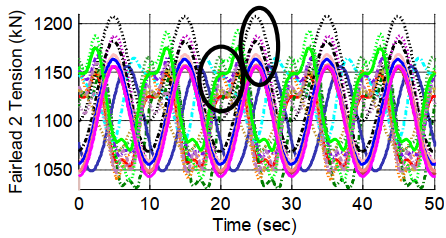
\includegraphics[width=1\textwidth]{2.1_fairten2.png}
        \caption{\small Fairlead 2 response for 2.1 (Robertson et al., 2014)}
        \label{fig:2.1_fairten2}
    \end{minipage}
    \hfill
    \begin{minipage}{0.51\textwidth}
        \centering
        \vspace{-0.3cm}
        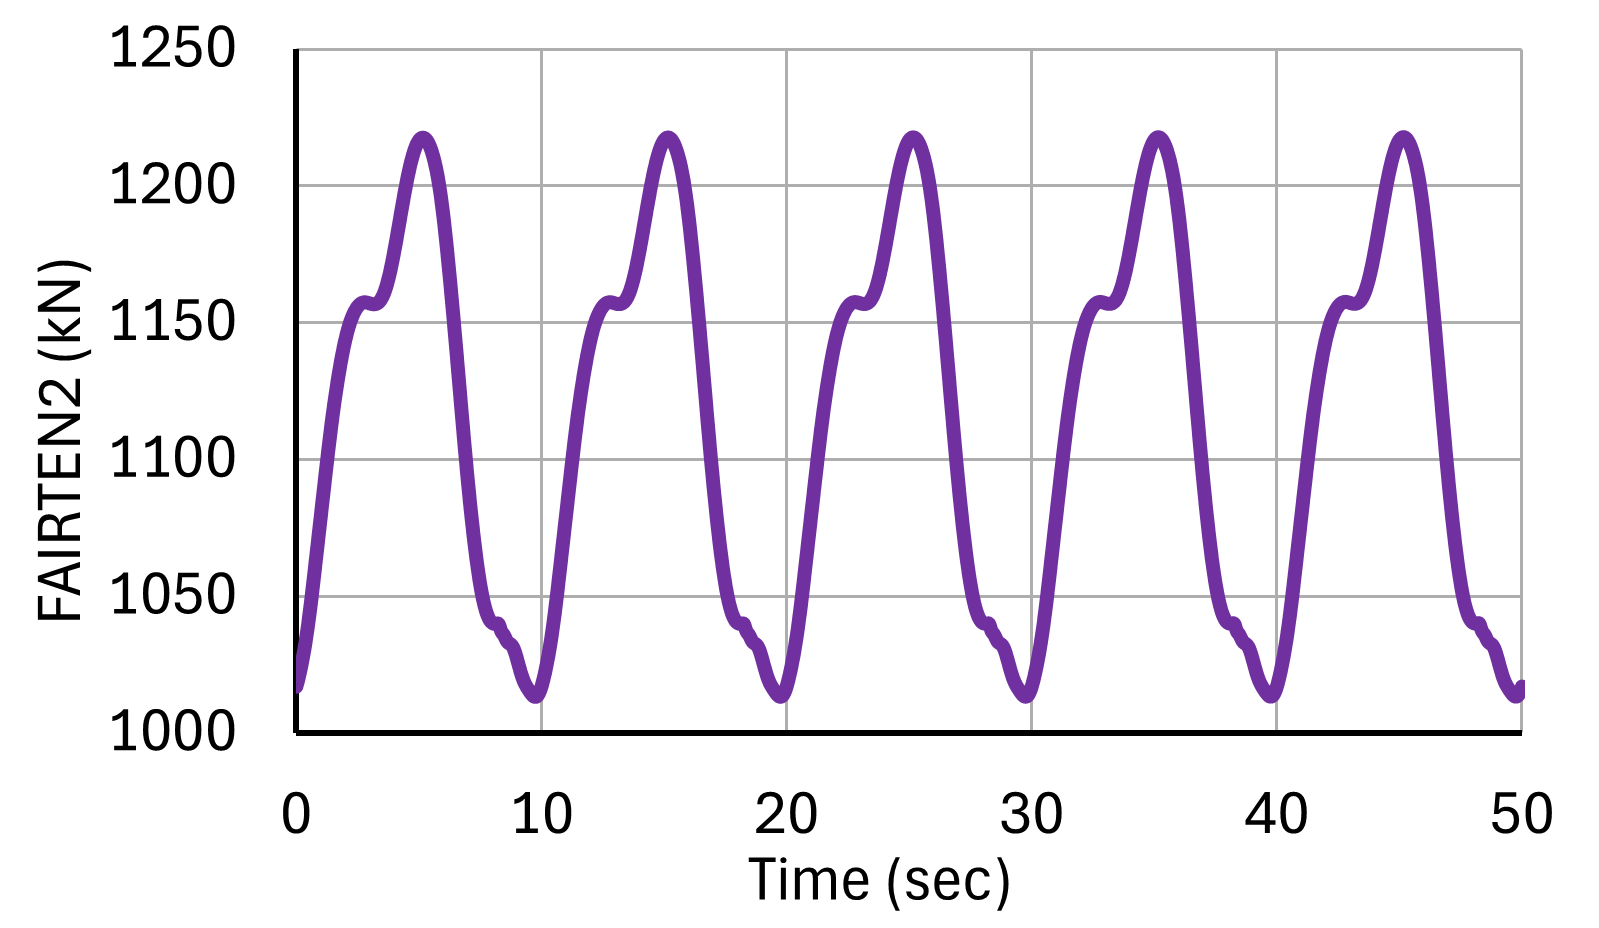
\includegraphics[width=0.95\textwidth]{2.1_fairten2_mine.png}
        \caption{\small Fairlead 2 response for 2.1}
        \label{fig:2.1_fairten2_mine}
    \end{minipage}
\end{figure}

\subsubsection{Load Case 2.2}

\hspace{0.5cm}Load case 2.2 analyzes the platform's response to irregular waves, examining surge motion, pitch motion, and tower bending moment. The reference study shows significant variation in average responses between participants (Figure 30), caused by different modeling approaches, particularly whether drift effects were included. Results processed through BEMRosetta compare simulations with and without quadratic transfer function (QTF) analysis (Figures 31-33).

Similar to load case 2.1, the results show that the surge motion is highly sensitive to second-order drift effects. In contrast, pitch motion and tower bending moment show minimal changes. The consistent patterns observed in this analysis match well with participant results when accounting for each study's specific modeling choices. 

\begin{figure}[H]
    \centering
    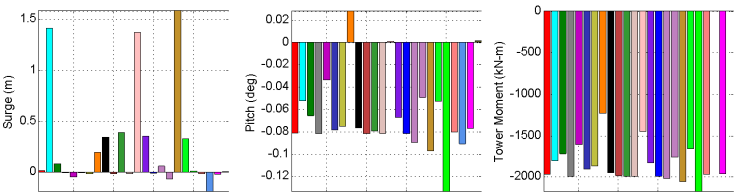
\includegraphics[width=1\textwidth]{2.2.png}
    \caption{\small Average responses to irregular waves (Robertson et al., 2014)}
    \label{fig:2.2}
\end{figure}

\begin{figure}[H]
    \centering
    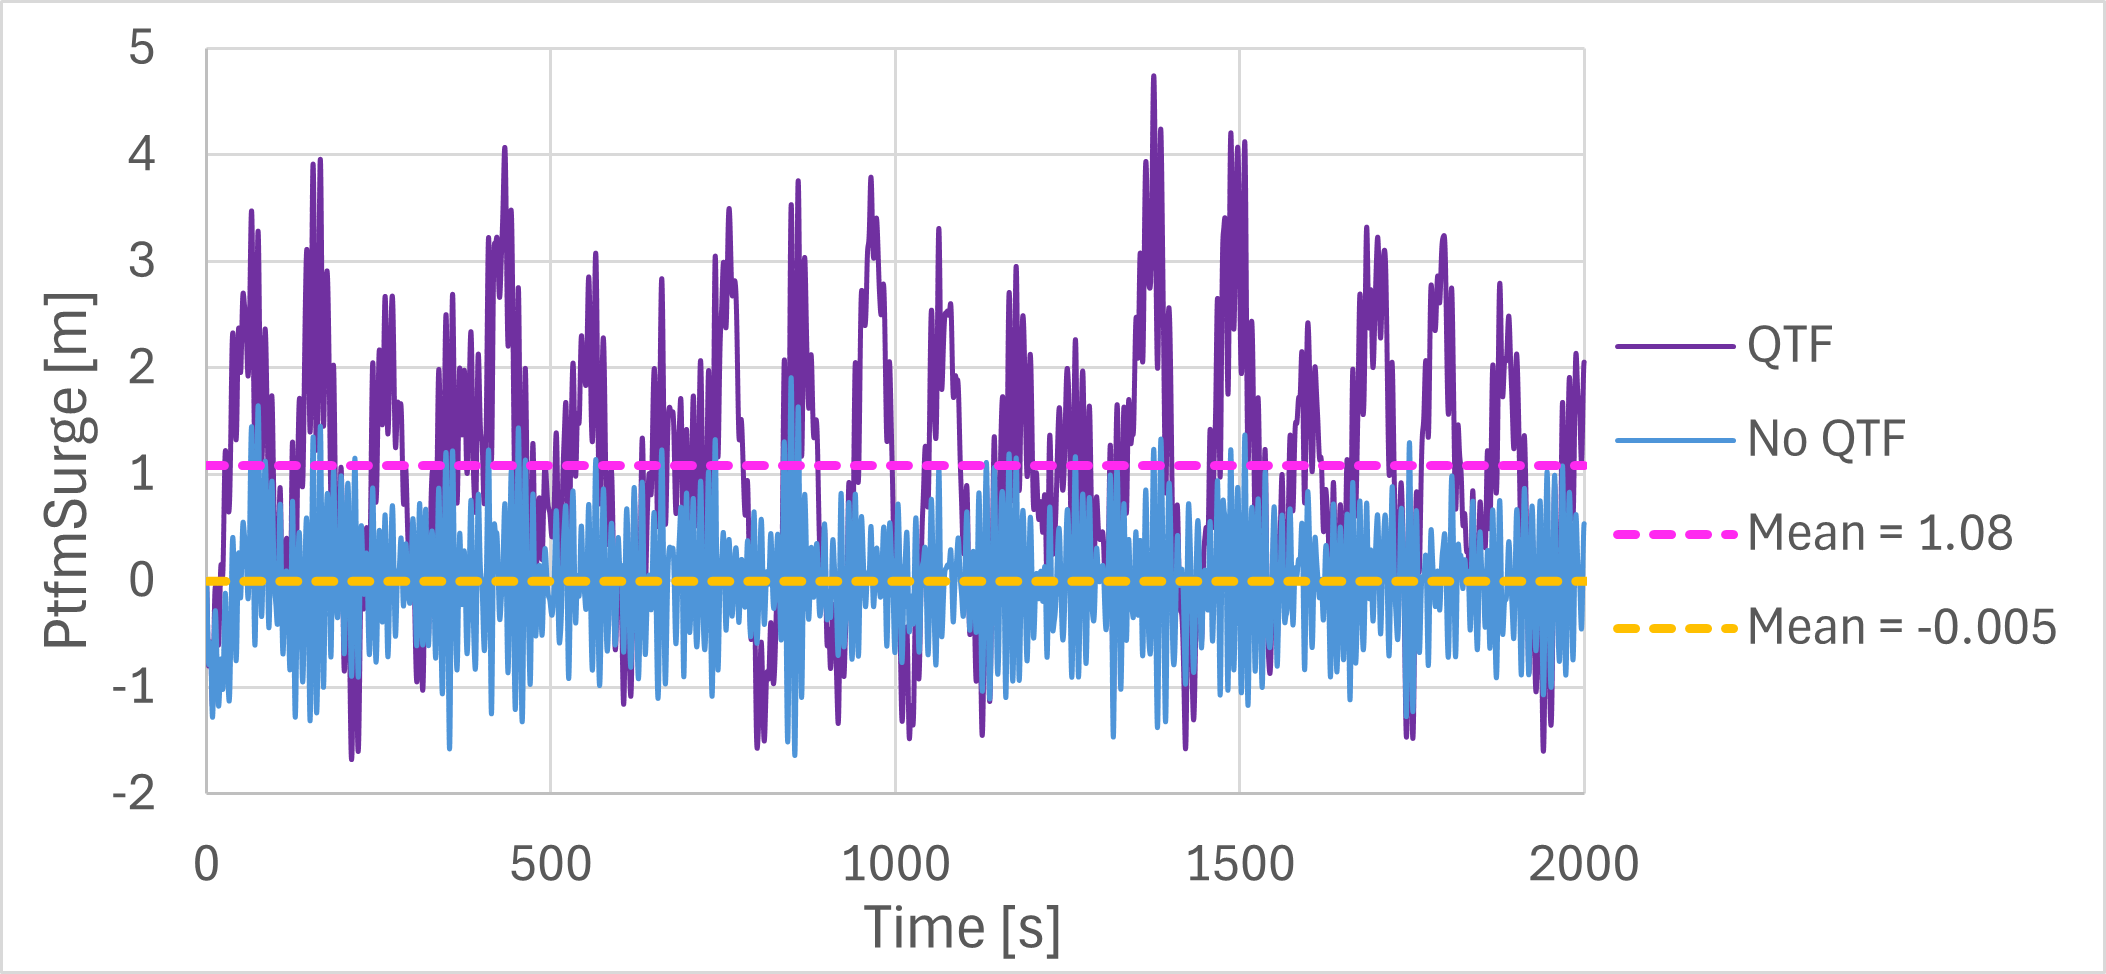
\includegraphics[width=0.78\textwidth]{2.2_surge.png}
    \caption{\small Surge response to irregular waves}
    \label{fig:2.2_surge}
\end{figure}

\begin{figure}[H]
    \centering
    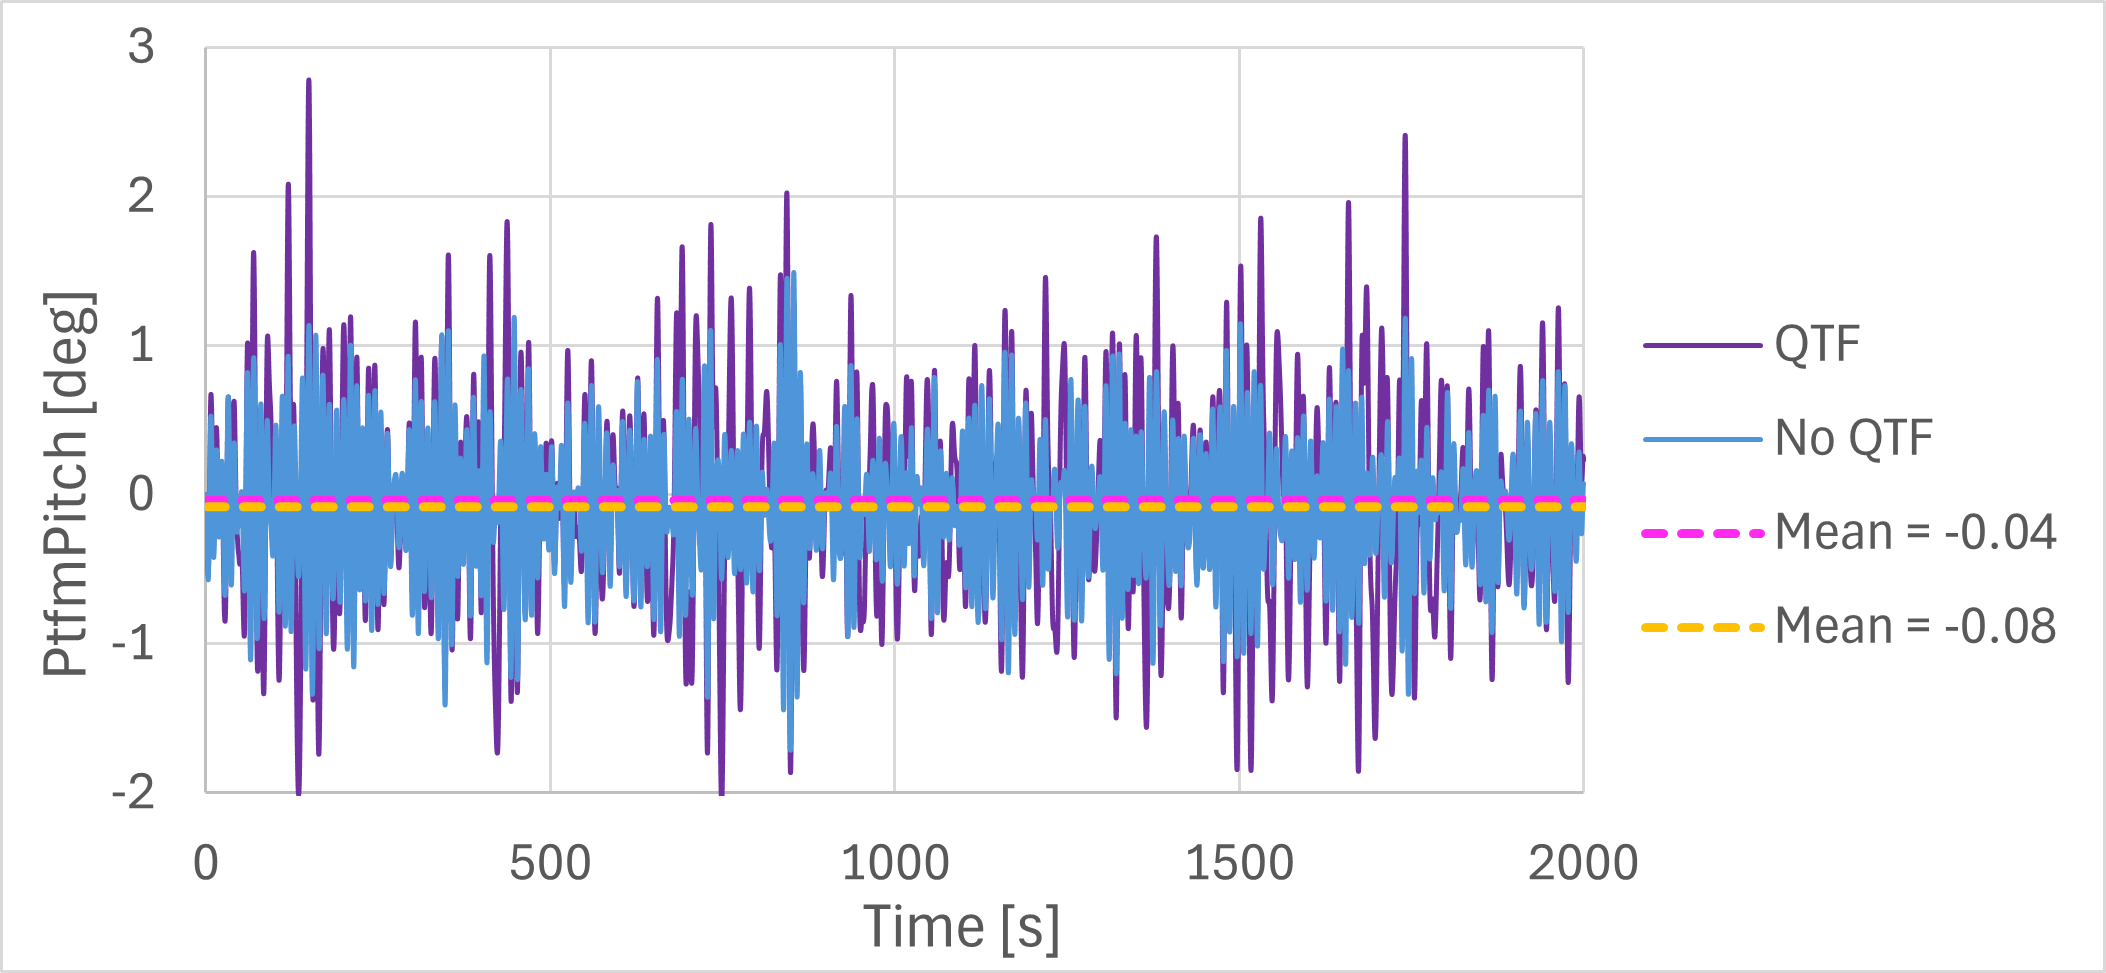
\includegraphics[width=0.78\textwidth]{2.2_pitch.png}
    \caption{\small Pitch response to irregular waves}
    \label{fig:2.2_pitch}
\end{figure}

\begin{figure}[H]
    \centering
    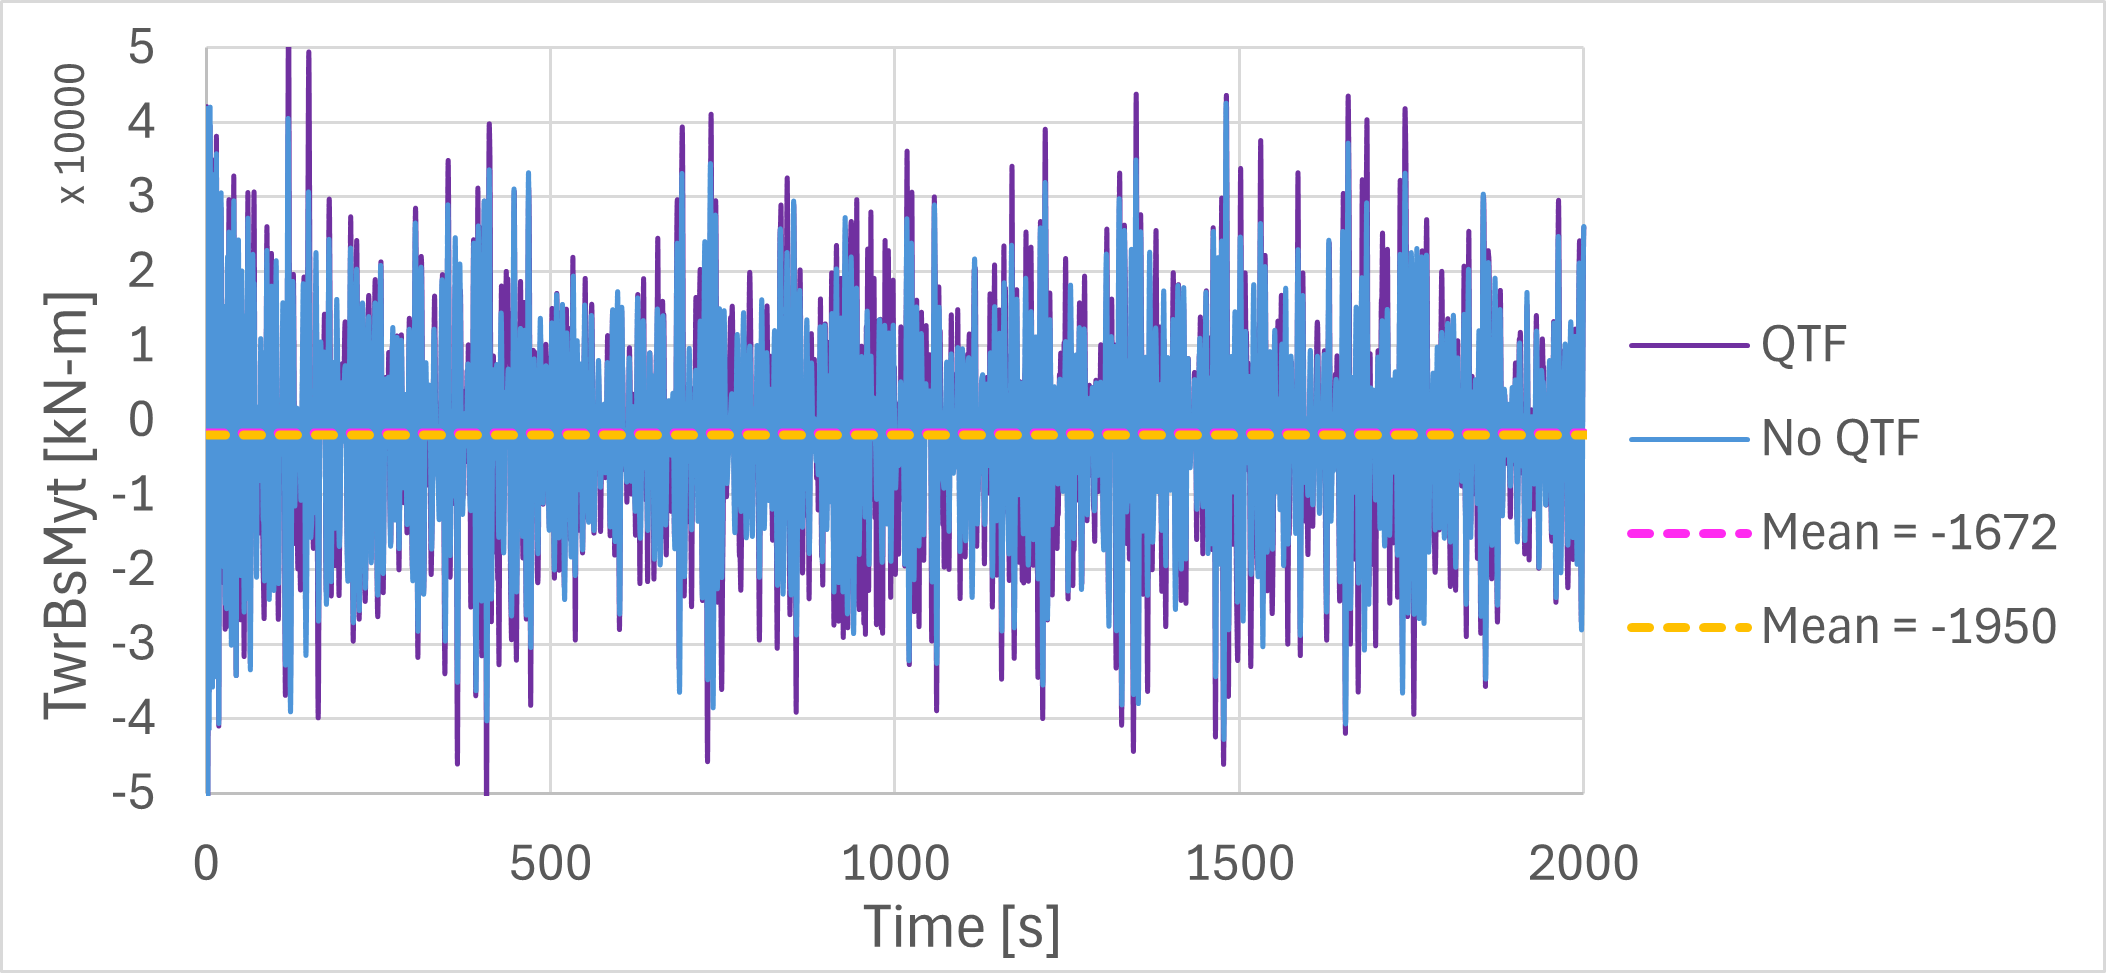
\includegraphics[width=0.78\textwidth]{2.2_twr.png}
    \caption{\small Tower bending response to irregular waves (fore/aft direction)}
    \label{fig:2.2_twr}
\end{figure}

\subsubsection{Load Case 2.4 \& 2.5}
\hspace{0.5cm}The load cases 2.4 and 2.5 were not analyzed in detail in the reference study. However, the results of these load cases were processed using BEMRosetta to extract the platform's response, comparing simulations with and without second-order drift effects using the QTF method.

Load case 2.4 represents operational conditions with regular waves that have a significant wave height of 6 meters and a wave period of 10 seconds, along with a surface current of 0.5 meters per second. Load case 2.5 examines extreme conditions characterized by irregular waves with a significant wave height of 50 meters and a wave period of 19.2 seconds.

The comparative results, presented in Figures 34-39, demonstrate that second-order drift effects impact platform response. Surge and pitch motions show higher sensitivity to these effects, particularly under the extreme wave conditions of load case 2.5. Heave motion, consistent with findings from previous load cases, remains relatively unaffected by the inclusion of second-order analysis.

\begin{figure}[H]
    \begin{minipage}{0.49\textwidth}
        \centering
        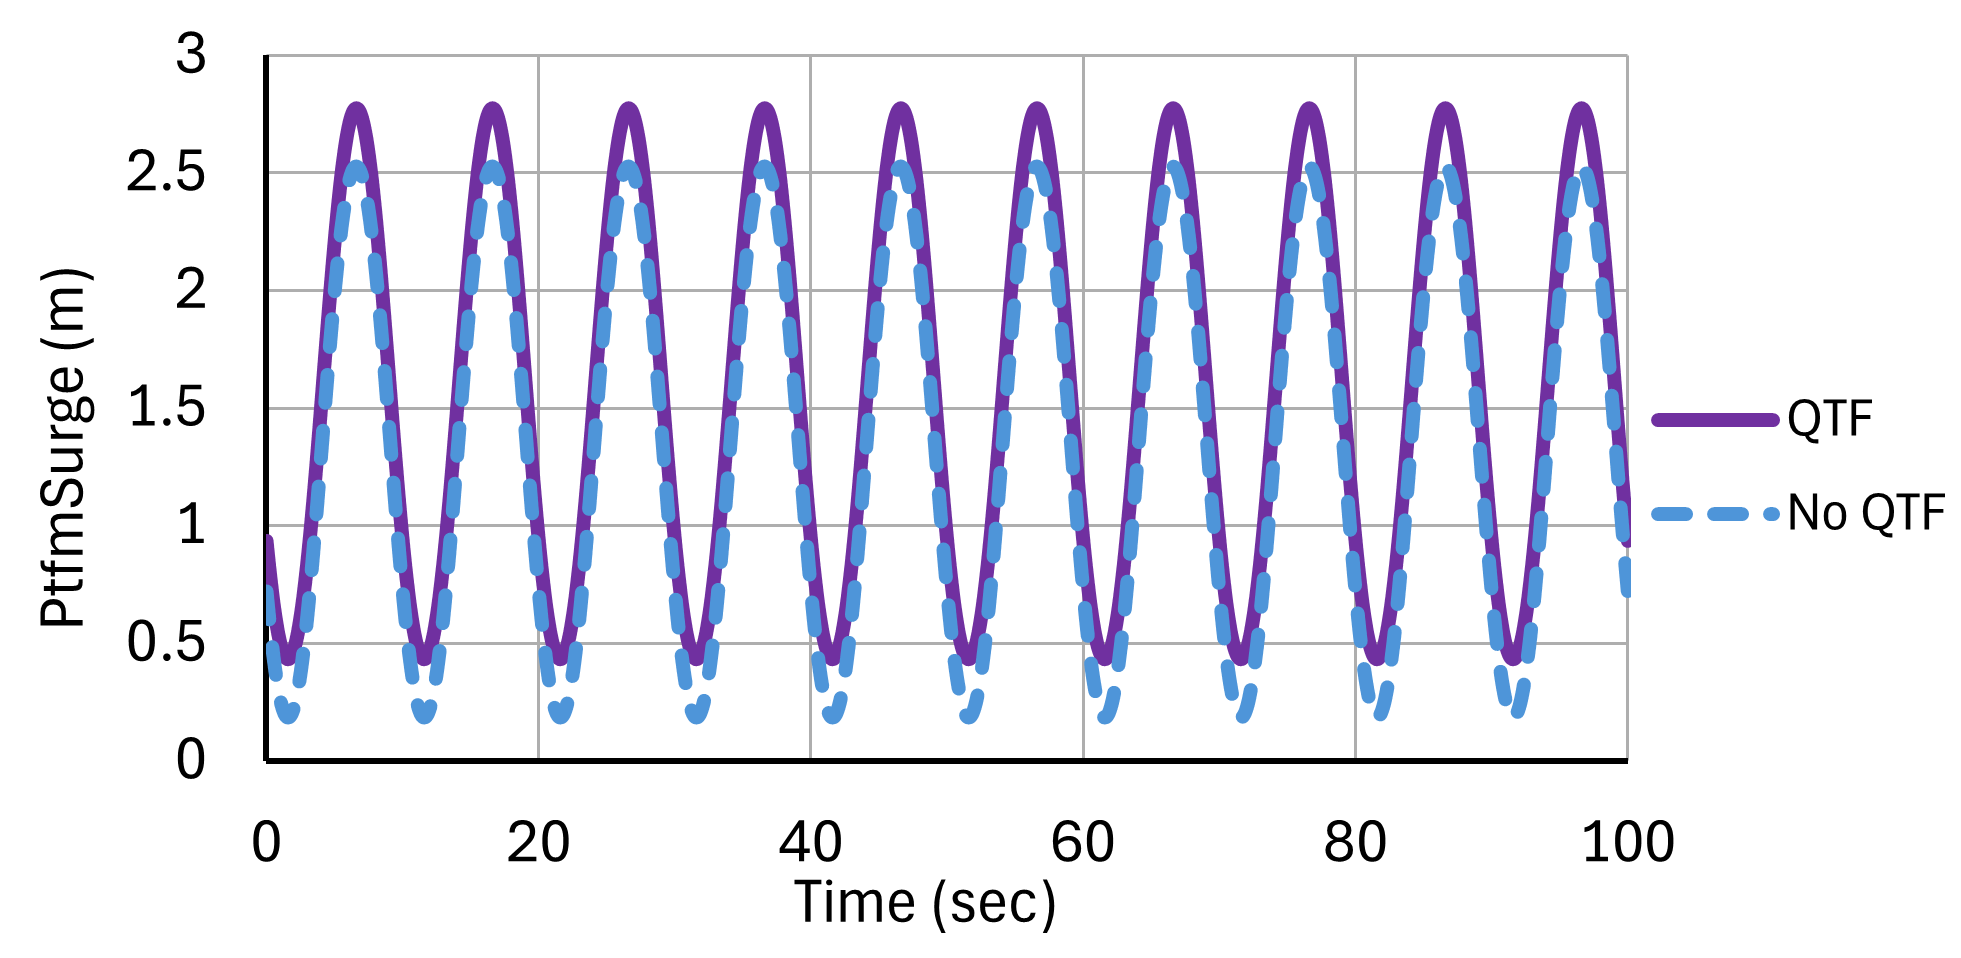
\includegraphics[width=1\textwidth]{2.4_surge.png}
        \caption{\small Surge response for 2.4} 
        \label{fig:2.4_surge}
    \end{minipage}
    \hfill
    \begin{minipage}{0.49\textwidth}
        \centering
        \vspace{-0.3cm}
        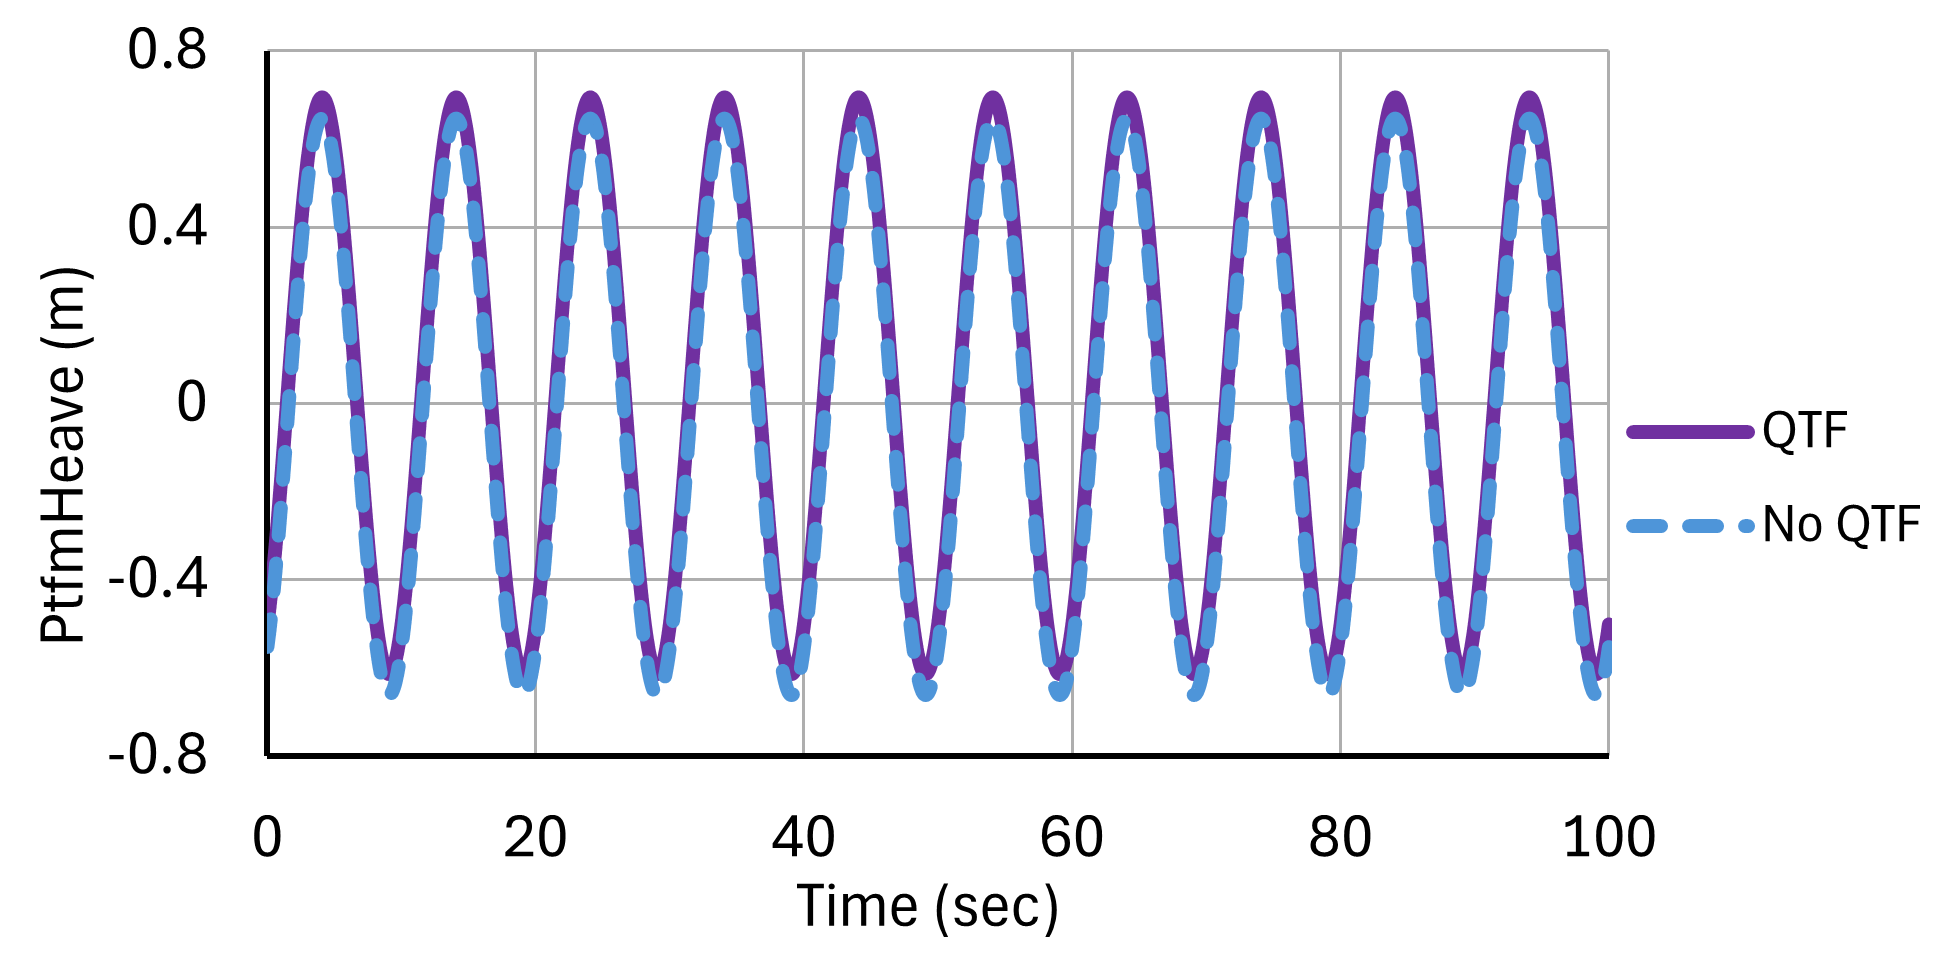
\includegraphics[width=1\textwidth]{2.4_heave.png}
        \caption{\small Heave response for 2.4}
        \label{fig:2.4_heave}
    \end{minipage}
\end{figure}

\begin{figure}[H]
    \begin{minipage}{0.49\textwidth}
        \centering
        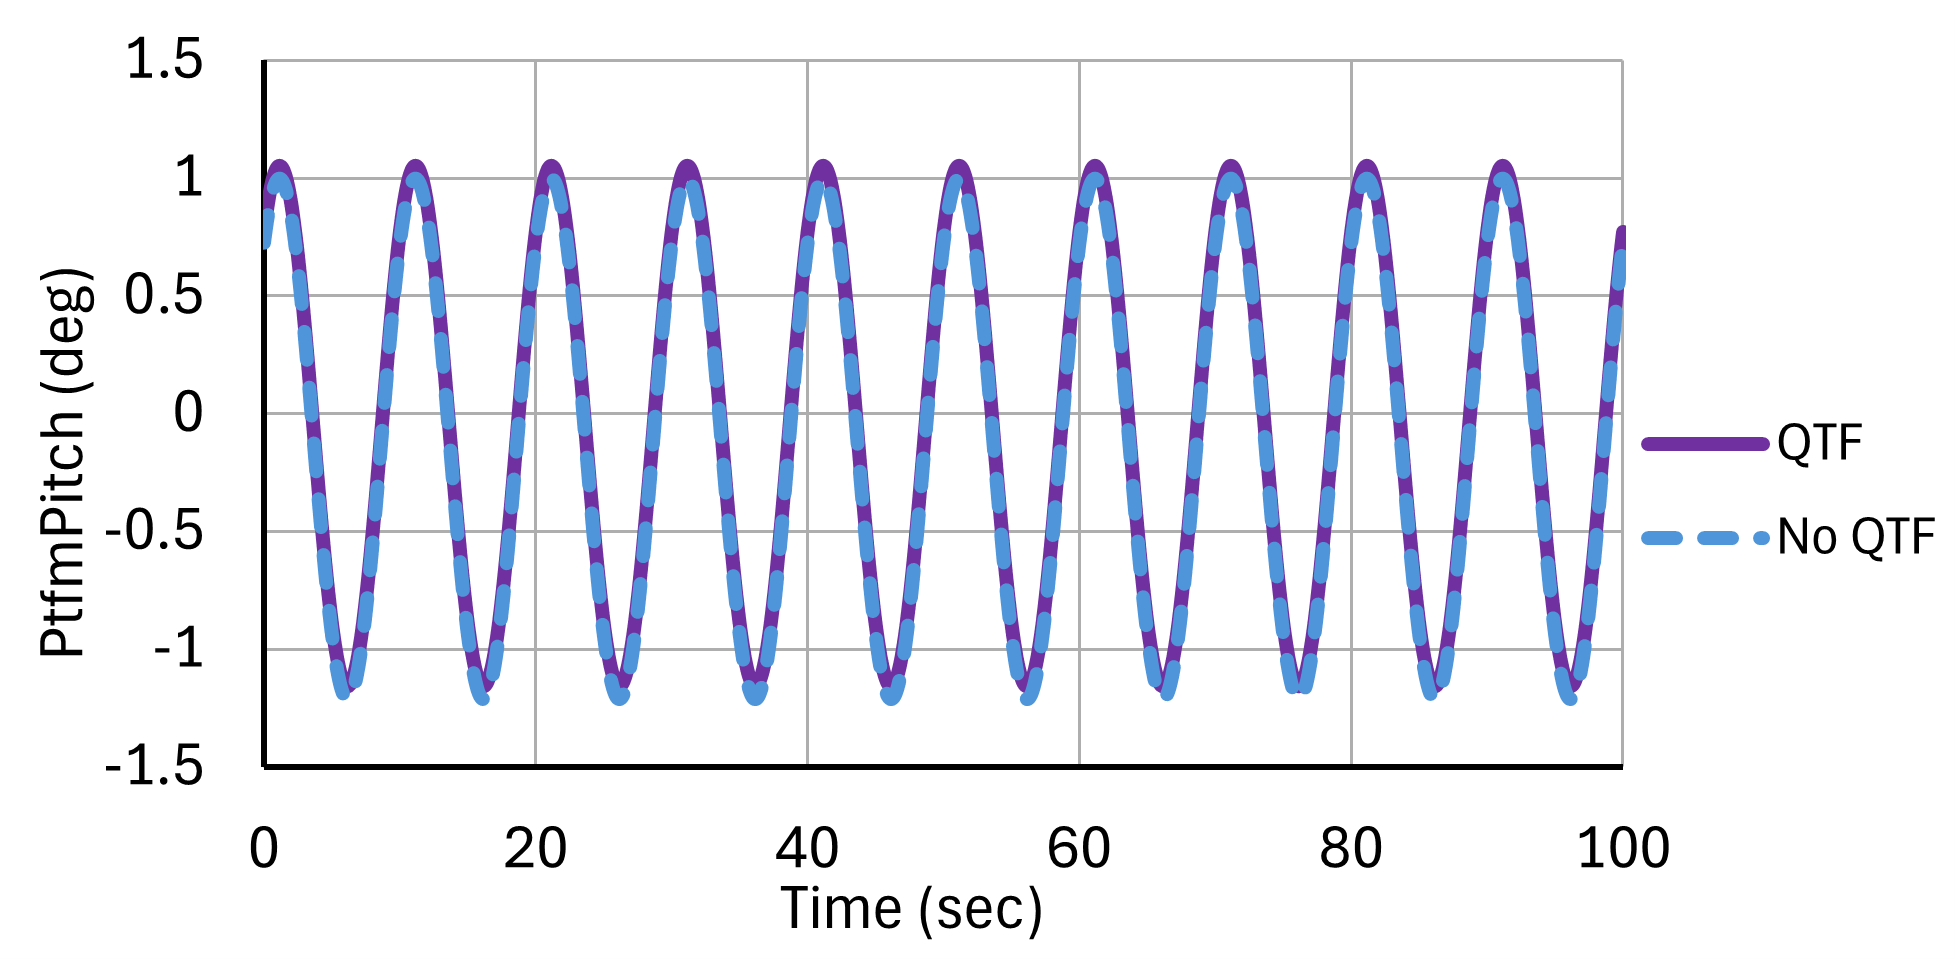
\includegraphics[width=1\textwidth]{2.4_pitch.png}
        \caption{\small Pitch response for 2.4} 
        \label{fig:2.4_pitch}
    \end{minipage}
    \hfill
    \begin{minipage}{0.49\textwidth}
        \centering
        \vspace{-0.3cm}
        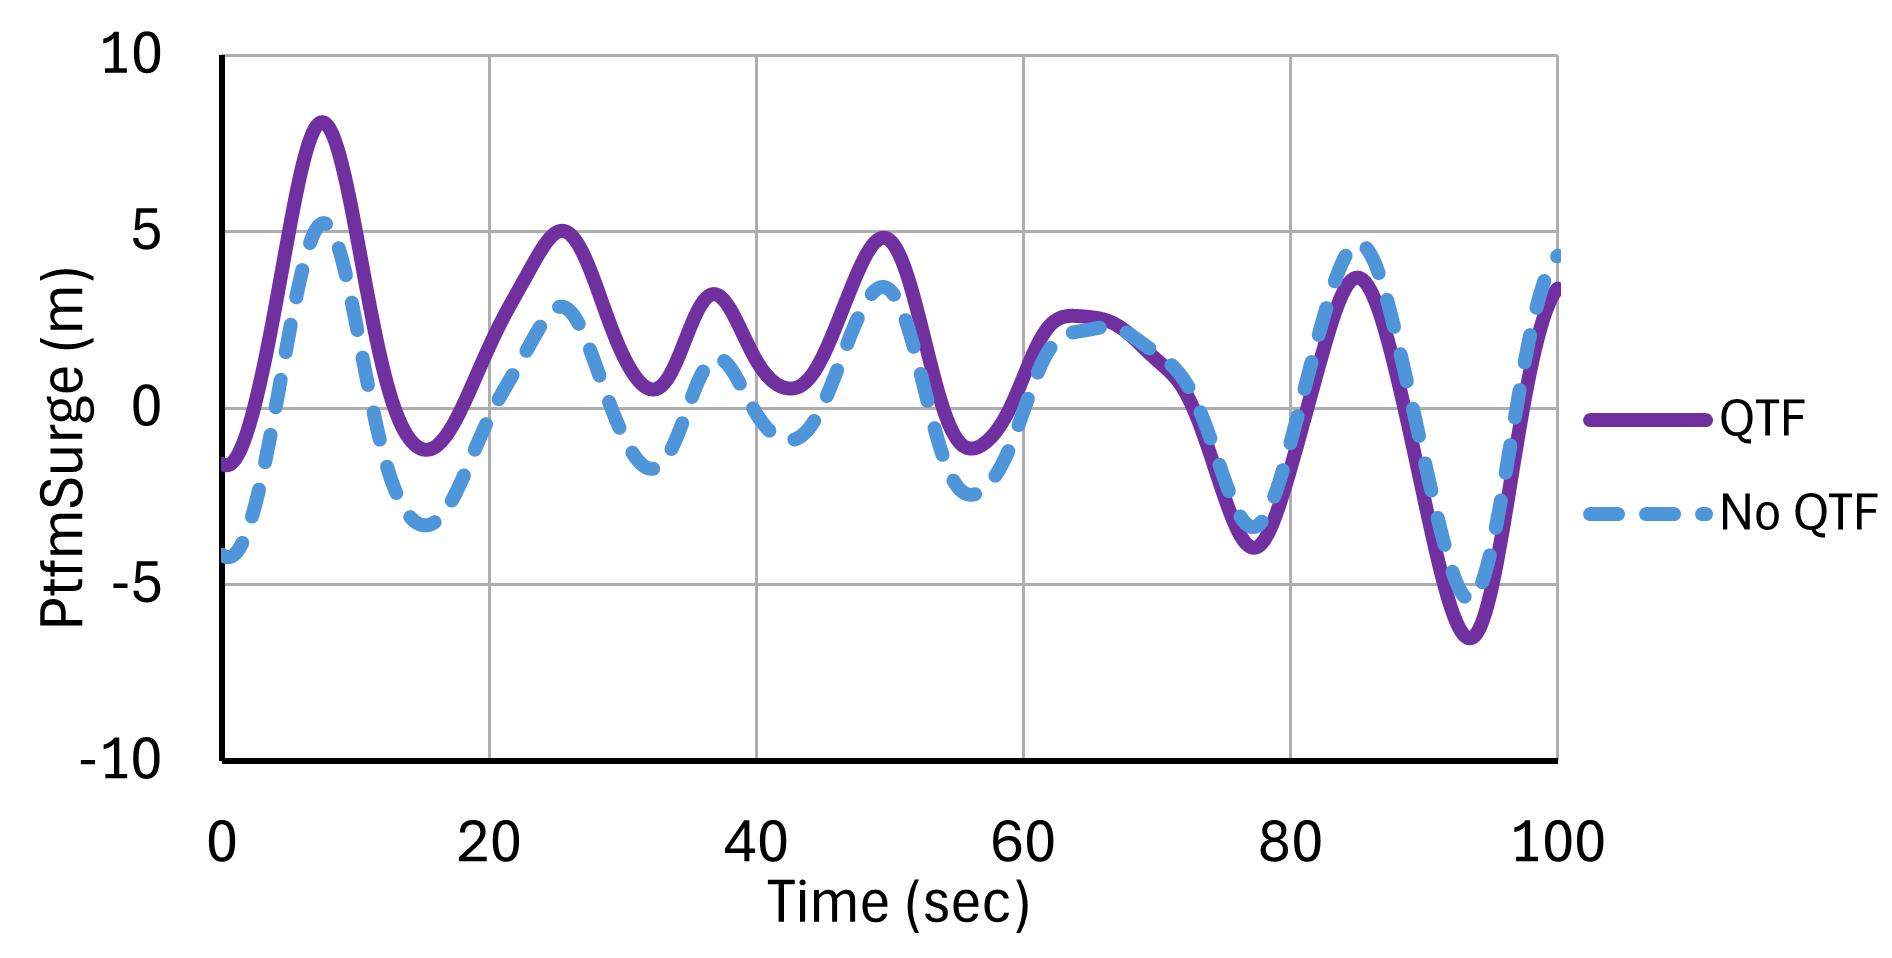
\includegraphics[width=1\textwidth]{2.5_surge.png}
        \caption{\small Surge response for 2.5}
        \label{fig:2.5_surge}
    \end{minipage}
\end{figure}

\begin{figure}[H]
    \begin{minipage}{0.49\textwidth}
        \centering
        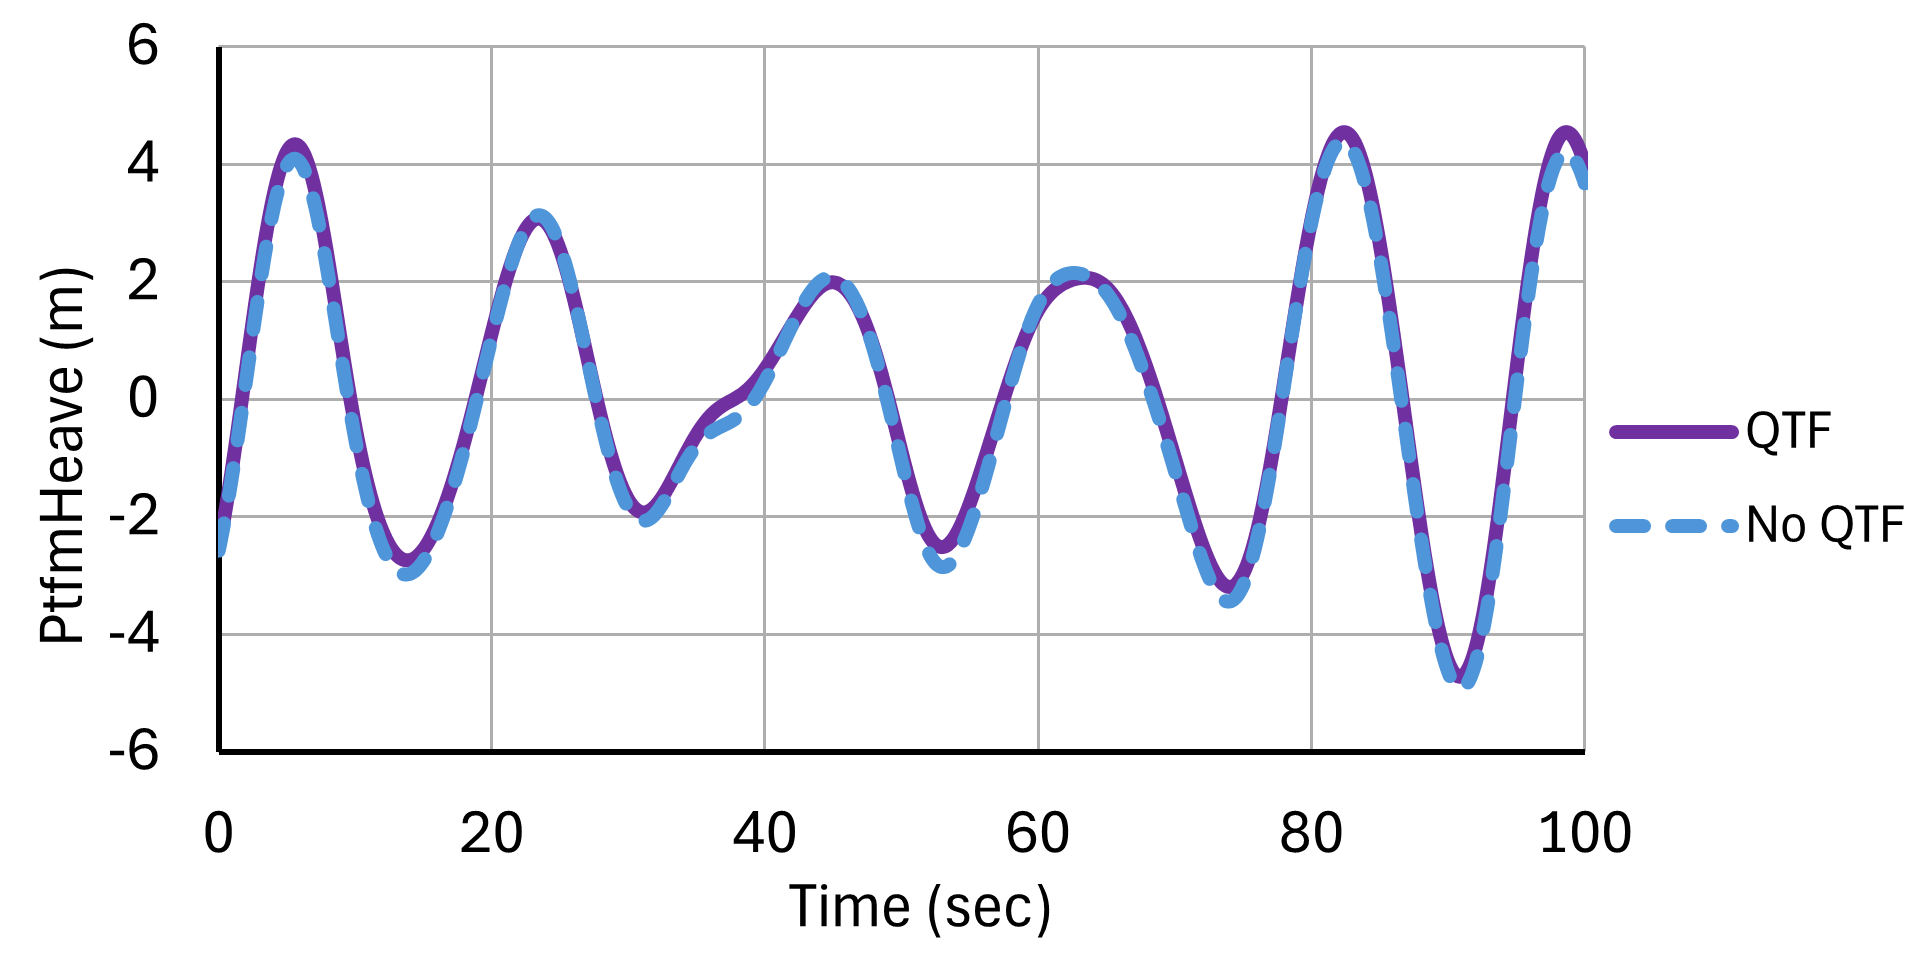
\includegraphics[width=1\textwidth]{2.5_heave.png}
        \caption{\small Heave response for 2.5}
        \label{fig:2.5_heave}
    \end{minipage}
    \hfill
    \begin{minipage}{0.49\textwidth}
        \centering
        \vspace{-0.3cm}
        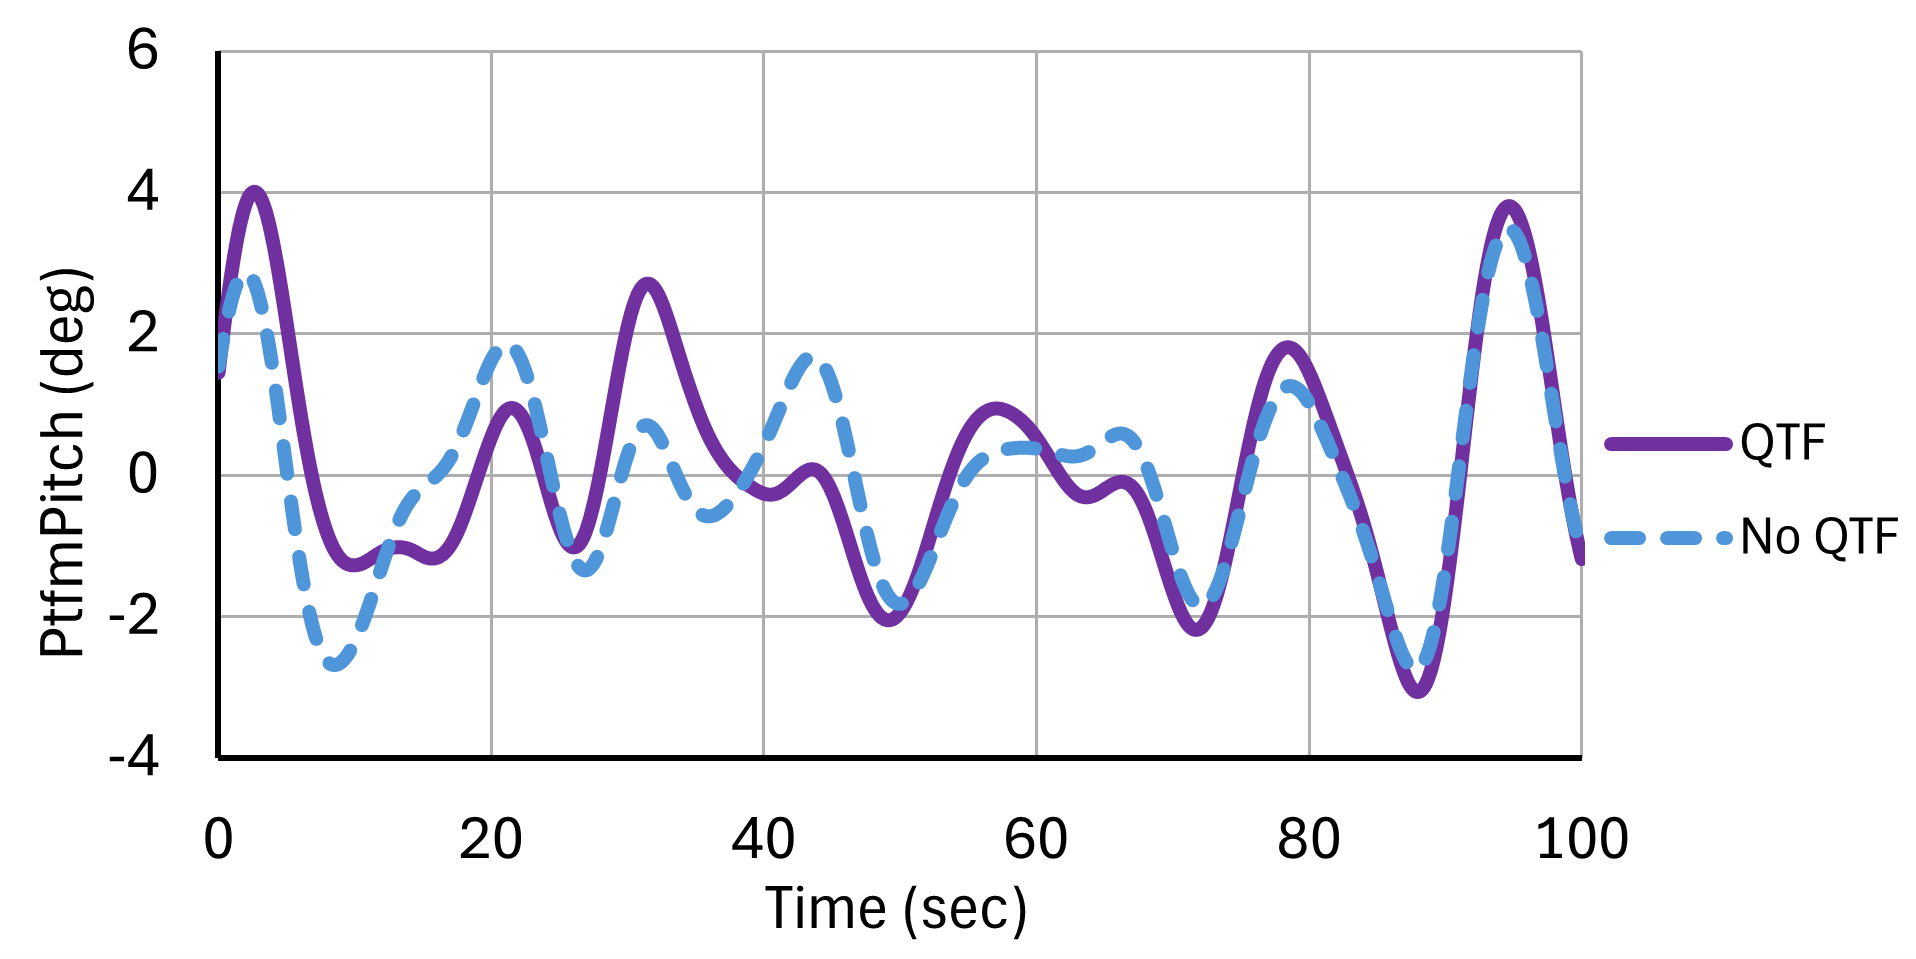
\includegraphics[width=1\textwidth]{2.5_pitch.png}
        \caption{\small Pitch response for 2.5}
        \label{fig:2.5_pitch}
    \end{minipage}
\end{figure}

\subsubsection{Load Case 2.6}
\hspace*{0.5cm}Load case 2.6 analyzes the platform's response to banded white noise to obtain Response Amplitudes Operators (RAOs) for the platform. RAOs represent the ratio of a system's response to the wave amplitude caused by wave excitation and are widely used to evaluate the linear wave-induced behavior of floating platforms in the frequency domain. For this study, the RAOs were calculated through dividing the each response PSD to the wave elevation PSD in the banded white-noise spectrum between 0.05 and 0.25 Hz and compared to the results from the reference study for both QTF (purple plot) and non-QTF (green plot) cases (Figures 40-55).

\begin{figure}[H]
    \centering
    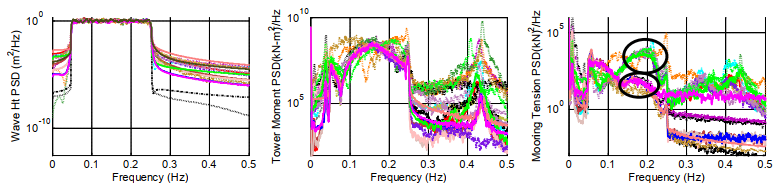
\includegraphics[width=1\textwidth]{w_t_t_p.png}
    \caption{\small Wave elevation, tower bending, and mooring tension PSD for load case 2.6 (Robertson et al., 2014)}
    \label{fig:w_t_t_p}
\end{figure}

\begin{figure}[H]
    \centering
    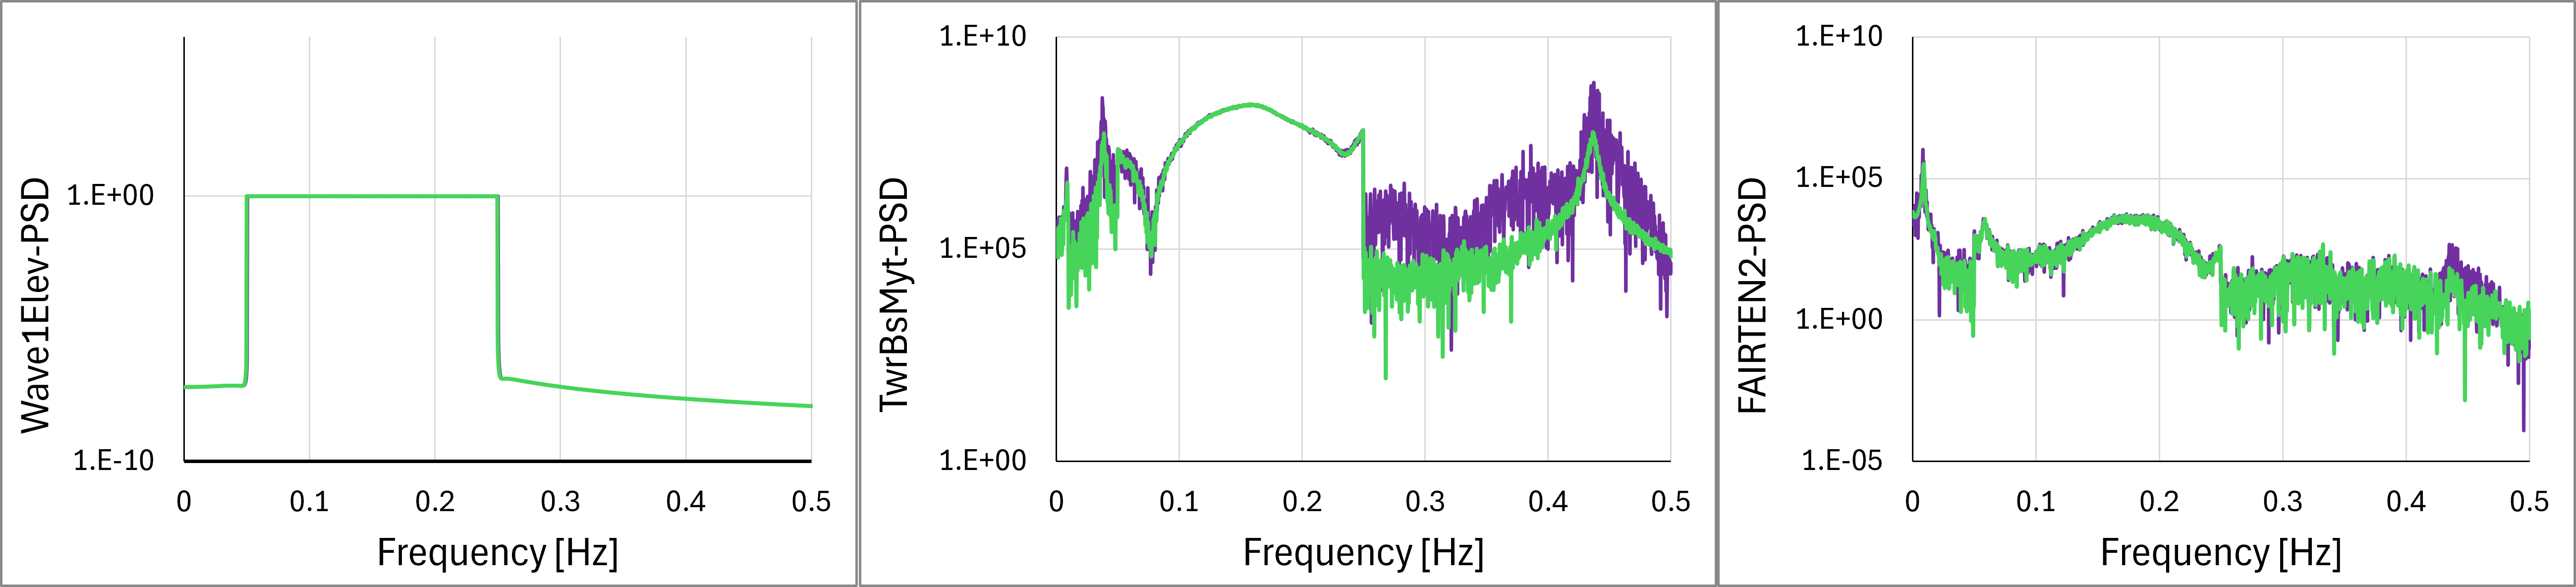
\includegraphics[width=1\textwidth]{wave_twr_ten_psd.png}
    \caption{\small Wave elevation, tower bending, and mooring tension PSD for load case 2.6}
    \label{fig:w_t_t_p_mine}
\end{figure}

\begin{figure}[H]
    \centering
    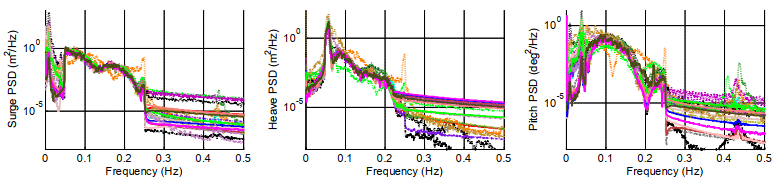
\includegraphics[width=1\textwidth]{s_h_p_p.png}
    \caption{\small Sugre, heave, and pitch PSD for load case 2.6 (Robertson et al., 2014)}
    \label{fig:s_h_p_p}
\end{figure}

\begin{figure}[H]
    \centering
    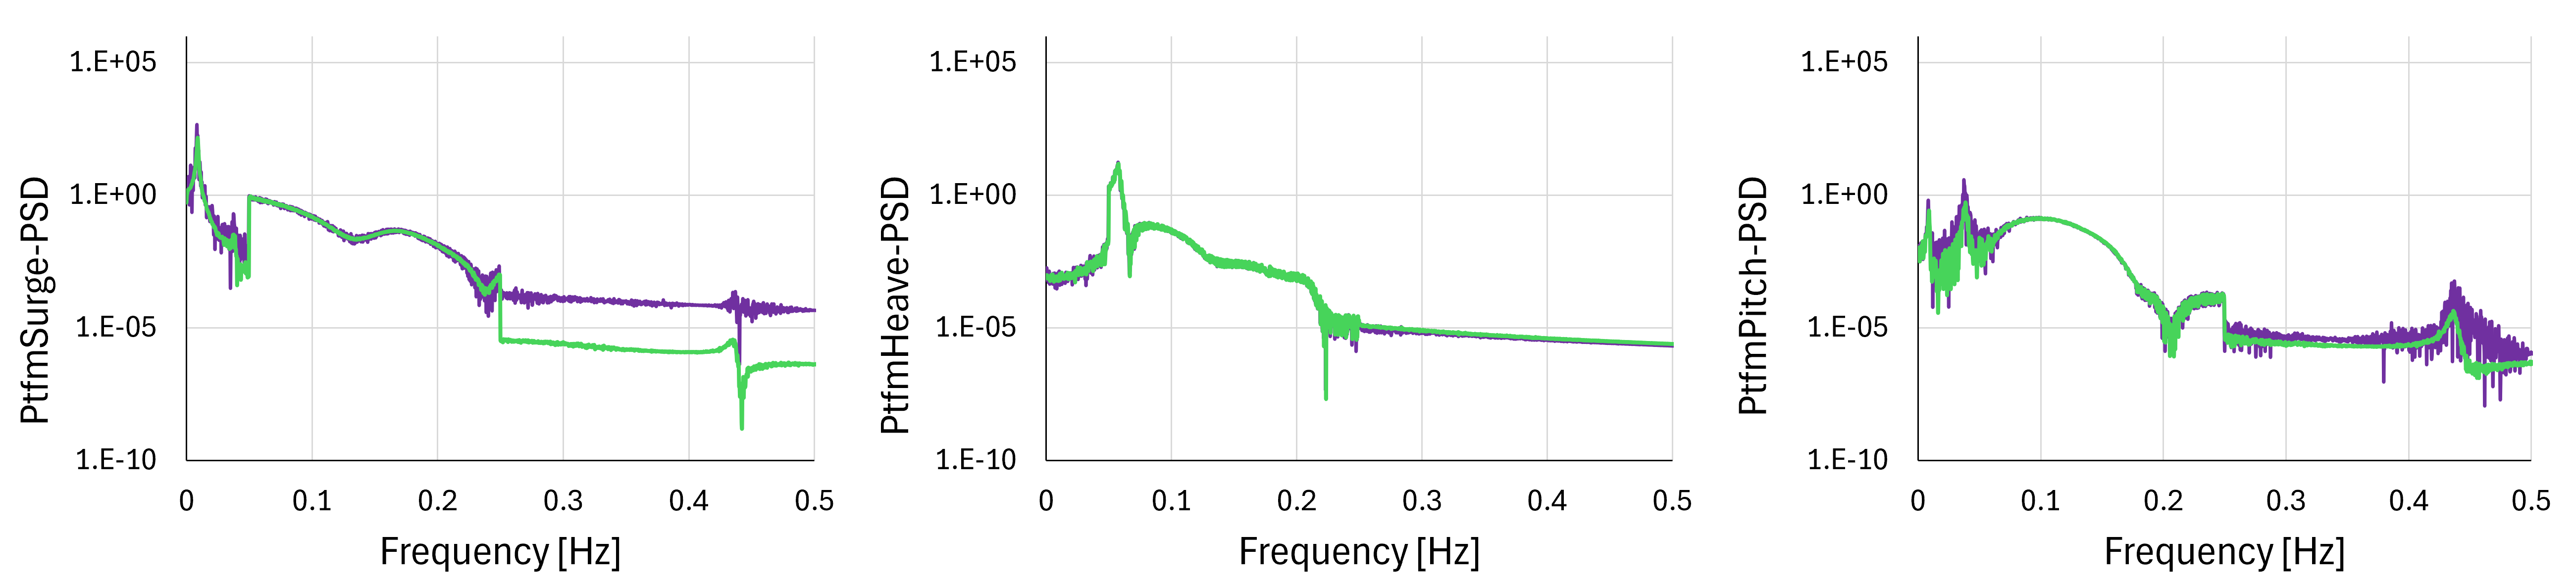
\includegraphics[width=1\textwidth]{sur_hea_pit_psd.png}
    \caption{\small Sugre, heave, and pitch PSD for load case 2.6}
    \label{fig:s_h_p_p_mine}
\end{figure}

\begin{figure}[H]
    \begin{minipage}{0.48\textwidth}
        \centering
        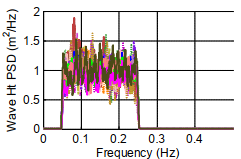
\includegraphics[width=1\textwidth]{2.6_wave.png}
        \caption{\small Wave elevation PSD for load case 2.6 (Robertson et al., 2014)} 
        \label{fig:2.6_wave}
    \end{minipage}
    \hfill
    \begin{minipage}{0.51\textwidth}
        \centering
        \vspace{-0.3cm}
        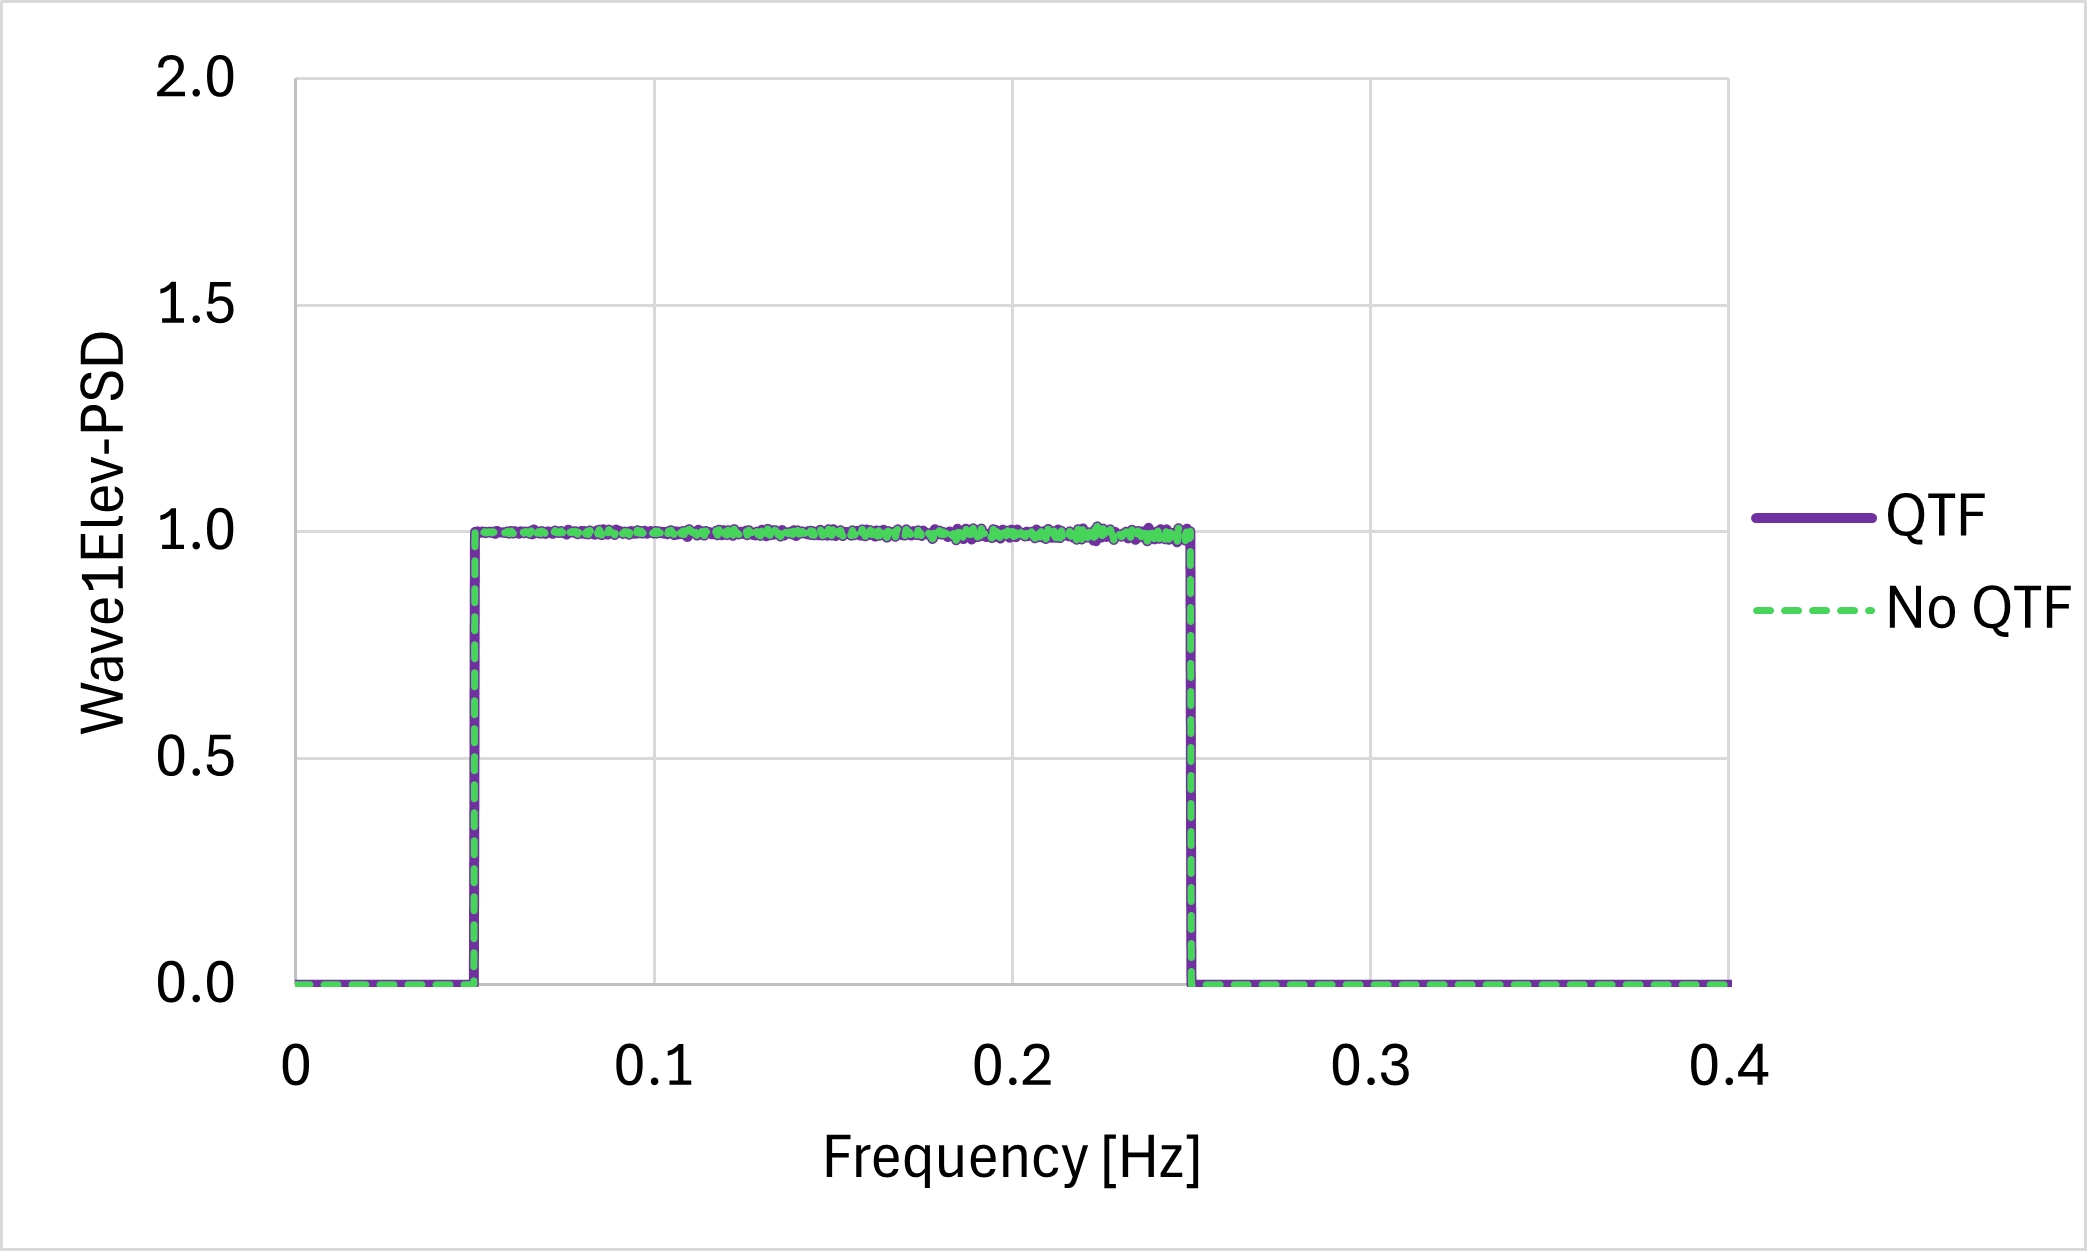
\includegraphics[width=1\textwidth]{2.6_wave_mine.png}
        \caption{\small Wave elevation PSD for load case 2.6}
        \label{fig:2.6_wave_mine}
    \end{minipage}
\end{figure}

\begin{figure}[H]
    \begin{minipage}{0.48\textwidth}
        \centering
        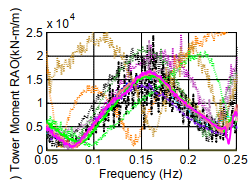
\includegraphics[width=0.95\textwidth]{2.6_twr.png}
        \caption{\small Tower bending moment RAO for load case 2.6 (Robertson et al., 2014)}
        \label{fig:2.6_twr}
    \end{minipage}
    \hfill
    \begin{minipage}{0.5\textwidth}
        \centering
        \vspace{0.6cm}
        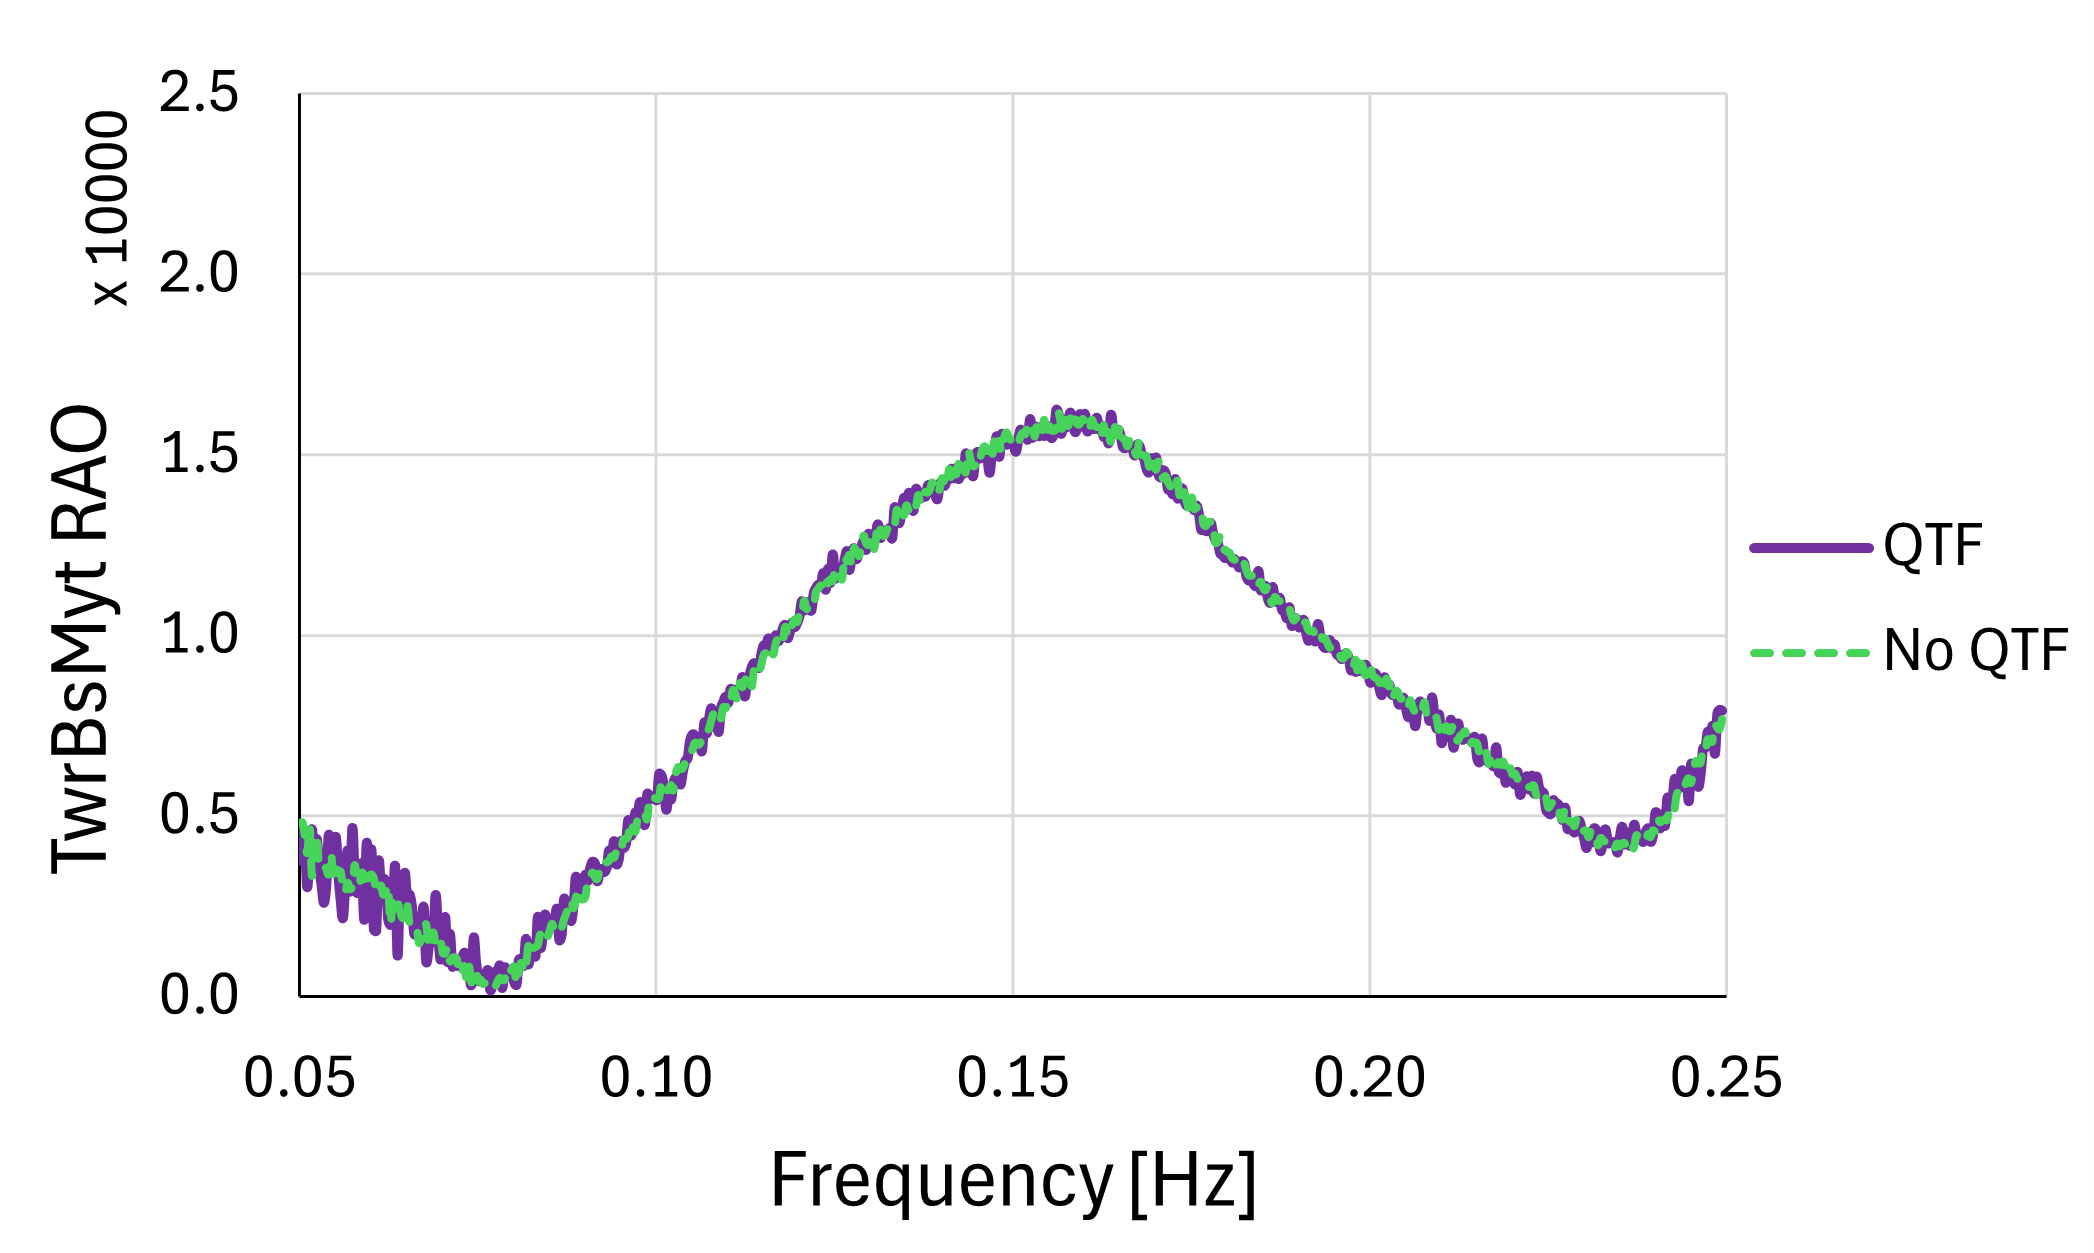
\includegraphics[width=1\textwidth]{2.6_twr_mine.png}
        \caption{\small Tower bending moment RAO for load case 2.6} 
        \label{fig:2.6_twr_mine}
    \end{minipage}
\end{figure}

\begin{figure}[H]
    \begin{minipage}{0.48\textwidth}
        \centering
        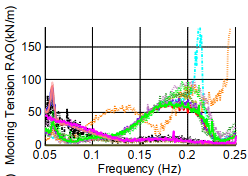
\includegraphics[width=1\textwidth]{2.6_ten.png}
        \caption{\small Mooring tension RAO for 2.6 (Robertson et al., 2014)}
        \label{fig:2.6_fairten2}
    \end{minipage}
    \hfill
    \begin{minipage}{0.5\textwidth}
        \centering
        \vspace{0.4cm}
        \includegraphics[width=1\textwidth]{2.6_ten_mine.png}
        \caption{\small Fairlead 2 RAO for 2.6}
        \label{fig:2.6_fairten2_mine}
    \end{minipage}
\end{figure}

\begin{figure}[H]
    \begin{minipage}{0.48\textwidth}
        \centering
        \includegraphics[width=1\textwidth]{2.6_surge.png}
        \caption{\small Surge RAO for load case 2.6 (Robertson et al., 2014)} 
        \label{fig:2.6_surge}
    \end{minipage}
    \hfill
    \begin{minipage}{0.5\textwidth}
        \centering
        \vspace{-0.2cm}
        \includegraphics[width=1\textwidth]{2.6_surge_mine.png}
        \caption{\small Surge RAO for load case 2.6}
        \label{fig:2.6_surge_mine}
    \end{minipage}
\end{figure}

\begin{figure}[H]
    \begin{minipage}{0.48\textwidth}
        \centering
        \includegraphics[width=1\textwidth]{2.6_heave.png}
        \caption{\small Heave RAO for load case 2.6 (Robertson et al., 2014)}
        \label{fig:2.6_heave}
    \end{minipage}
    \hfill
    \begin{minipage}{0.5\textwidth}
        \centering
        \includegraphics[width=1\textwidth]{2.6_heave_mine.png}
        \caption{\small Heave RAO for load case 2.6} 
        \label{fig:2.6_heave_mine}
    \end{minipage}
\end{figure}

\begin{figure}[H]
    \begin{minipage}{0.48\textwidth}
        \centering
        \includegraphics[width=1\textwidth]{2.6_pitch.png}
        \caption{\small Pitch RAO for 2.6 (Robertson et al., 2014)}
        \label{fig:2.6_pitch}
    \end{minipage}
    \hfill
    \begin{minipage}{0.5\textwidth}
        \centering
        \includegraphics[width=1\textwidth]{2.6_pitch_mine.png}
        \caption{\small Pitch RAO for 2.6}
        \label{fig:2.6_pitch_mine}
    \end{minipage}
\end{figure}

Both the PSD and RAO graphs show a good agreement with the reference study, particularly the non-QTF case with less oscillations in the surge, heave, and pitch responses. The QTF case shows more oscillations overall, which is expected as the QTF method accounts for second-order drift effects. From the PSD graphs, it can be seen that the natural frequency of heave, being around 0.058 Hz (Figure 53), falls within the wave excitation frequency range, leading to a significant increase in the chance of resonance. This is also reflected in the heave RAO graph, showing the peak to be over 4 m/m. The peaks for the rest of the responses are outside of this range, indicating that they are less sensitive to wave excitation. 

\newpage
\section{Recreated Platform Model Analysis}

\hspace*{0.5cm}The OC4 semisubmersible platform was recreated independently using Rhino (Figure 56), and the WAMIT files of this model were created using the HAMS software. In Figures 57 and 58, the hydrostatic matrices of the models can be seen. The matrix for the recreated model includes some coupling forces caused by the meshing process. This results in slight differences between the outputs of the cases, which will be discussed in their respective sections. The same load cases were applied to the recreated model in OpenFAST, allowing for a direct comparison between the pre-existing (presented as the purple plot named "Ex") and recreated models (presented as the blue plot named "Re"). The comparison is done using the case without including the second-drift effects for the pre-existing model, as the HAMS software does not provide the required WAMIT outputs to use the QTF method.

\begin{figure}[H]
    \centering
    \includegraphics[width=1\textwidth]{rhino.png}
    \caption{\small Recreated OC4 semisubmersible platform in Rhino}
    \label{fig:rhino}
\end{figure}

\begin{figure}[H]
    \centering
    \includegraphics[width=0.95\textwidth]{hyd_st_org.png}
    \caption{\small Hydrostatic matrix of the pre-existing model}
    \label{fig:hyd_st_org}
\end{figure}

\begin{figure}[H]
    \centering
    \includegraphics[width=0.95\textwidth]{hyd_st_re.png}
    \caption{\small Hydrostatic matrix of the recreated model}
    \label{fig:hyd_st_re}
\end{figure}

\subsection{Free Decay Tests}
\hspace*{0.5cm}The free decay tests were conducted on the recreated model, and the results were compared to those obtained from the pre-existing model (Figures 35-40). The natural frequencies were extracted from the time-domain data using the Fast Fourier Transform (FFT) method on BEMRosetta. (Figures 59-64). 

\begin{figure}[H]
    \begin{minipage}{0.47\textwidth}
        \centering
        \includegraphics[width=1\textwidth]{1.3_surge_mine.png}
        \caption{\small Surge free decay platform motion response for 1.3a (recreated model vs. pre-existing model)}
        \label{fig:1.3a_surge_mine_recreated}
    \end{minipage}
    \hfill
    \begin{minipage}{0.49\textwidth}
        \centering
        \includegraphics[width=0.95\textwidth]{1.3a_heave_mine_1.png}
        \caption{\small Heave free decay platform motion response for 1.3a (recreated model vs. pre-existing model)}
        \label{fig:1.3a_heave_mine_recreated}
    \end{minipage}
\end{figure}

\begin{figure}[H]
    \begin{minipage}{0.47\textwidth}
        \centering
        \includegraphics[width=1\textwidth]{1.3a_pitch_mine_1.png}
        \caption{\small Pitch free decay platform motion response for 1.3a (recreated model vs. pre-existing model)}
        \label{fig:1.3a_pitch_mine_recreated}
    \end{minipage}
    \hfill
    \begin{minipage}{0.49\textwidth}
        \centering
        \includegraphics[width=0.95\textwidth]{1.3b_surge_mine_1.png}
        \caption{\small Surge free decay platform motion response for 1.3b (recreated model vs. pre-existing model)}
        \label{fig:1.3b_surge_mine_recreated}
    \end{minipage}
\end{figure}

\begin{figure}[H]
    \begin{minipage}{0.47\textwidth}
        \centering
        \includegraphics[width=1\textwidth]{1.3b_heave_mine_1.png}
        \caption{\small Heave free decay platform motion response for 1.3b (recreated model vs. pre-existing model)}
        \label{fig:1.3b_heave_mine_recreated}
    \end{minipage}
    \hfill
    \begin{minipage}{0.49\textwidth}
        \centering
        \includegraphics[width=0.95\textwidth]{1.3b_pitch_mine_1.png}
        \caption{\small Pitch free decay platform motion response for 1.3b (recreated model vs. pre-existing model)}
        \label{fig:1.3b_pitch_mine_recreated}
    \end{minipage}
\end{figure}

The graphs plotted for the surge motion in both load cases shows a very close resemblance to the pre-existing model, whereas the pitch and especially heave motion response shows differences in the amplitude of the oscillations. This is due to the differences in the modeling approaches and the volume calculated for the submerged part of the platform from the recreated model. The recreated model was created to closely match the dimensions and properties of the pre-existing model, but slight variations in the geometry may have led to these differences in response. The original model had a volume of 13,917 m³, while the recreated model had a volume of 13,603 m³. The difference in volume causes the bouyancy force to be different, which directly affects the heave motion response. The recreated model's heave motion response shows a higher amplitude than the pre-existing model, since the volume of the body is smaller. On the heave plot for the load case 1.3a, the green colored line represents the recreated model with the volume kept same as the original model (Figure 63). For this case, the recreated model's heave motion response is very close to the pre-existing model, confirming that the volume of the submerged part of the platform is a significant factor in determining the heave motion response. The recreated model's pitch motion response is also affected by the volume difference, but to a lesser extent than the heave motion response, which is presumably due to coupling effects.

%%nat frequencies recreated model
\begin{figure}[H]
    \begin{minipage}{0.47\textwidth}
        \centering
        \includegraphics[width=1\textwidth]{nat_freq_sway_1.png}
        \caption{\small Sway natural frequency (recreated model vs. pre-existing model)}
        \label{fig:nat_freq_sway_recreated}
    \end{minipage}
    \hfill
    \begin{minipage}{0.48\textwidth}
        \centering
        \includegraphics[width=1\textwidth]{nat_freq_surge_1.png}
        \caption{\small Surge natural frequency (recreated model vs. pre-existing model)}
        \label{fig:nat_freq_surge_recreated}
    \end{minipage}
\end{figure}

\begin{figure}[H]
    \begin{minipage}{0.47\textwidth}
        \centering
        \includegraphics[width=1\textwidth]{nat_freq_heave_1.png}
        \caption{\small Heave natural frequency (recreated model vs. pre-existing model)}
        \label{fig:nat_freq_heave_recreated}
    \end{minipage}
    \hfill
    \begin{minipage}{0.48\textwidth}
        \centering
        \includegraphics[width=1\textwidth]{nat_freq_roll_1.png}
        \caption{\small Roll natural frequency (recreated model vs. pre-existing model)}
        \label{fig:nat_freq_roll_recreated}
    \end{minipage}
\end{figure}

\begin{figure}[H]
    \begin{minipage}{0.47\textwidth}
        \centering
        \includegraphics[width=1\textwidth]{nat_freq_pitch_1.png}
        \caption{\small Pitch natural frequency (recreated model vs. pre-existing model)}
        \label{fig:nat_freq_pitch_recreated}
    \end{minipage}
    \hfill
    \begin{minipage}{0.48\textwidth}
        \centering
        \includegraphics[width=1\textwidth]{nat_freq_yaw_1.png}
        \caption{\small Yaw natural frequency (recreated model vs. pre-existing model)}
        \label{fig:nat_freq_yaw_recreated}
    \end{minipage}
\end{figure}


The natural frequencies extracted from the time-domain data using the Fast Fourier Transform (FFT) method on BEMRosetta were consistent with those obtained from the pre-existing model, confirming the accuracy of the recreated model. As discussed previously, the heave motion shows some difference in natural frequency, which is due to the difference in the volume of the submerged part of the platform (Figure 67). The recreated model's heave natural frequency is lower than the pre-existing model's, which is consistent with the heave motion response. Additionally, the yaw motion also presents a slight difference, which is likely a result of the different hydrostatic matrices caused by the modelling process (Figure 70). The other degrees of freedom show very close results to the pre-existing model.

\subsection{Wave and Current Induced Tests}

\hspace*{0.5cm}The wave-induced responses were analyzed by applying regular and irregular waves to the recreated model. The peak period of the waves were taken as 10 seconds, and the significant wave height was set to 6 meters. For the irregular waves, the JONSWAP spectrum was used to generate the wave field, with a peak wave shape parameter of 2.87. The results were compared to those obtained from the pre-existing model (No QTF case).

\subsubsection{Load Case 2.1}
\hspace*{0.5cm}The load case 2.1 was used to analyze the platform’s response to regular waves, focusing on heave, pitch, surge motions, and the tension force at fairlead 2. The analysis was conducted using the pre-existing model and the recreated model and compared (Figures 71-74).

\begin{figure}[H]
    \begin{minipage}{0.48\textwidth}
        \centering
        \includegraphics[width=1\textwidth]{2.1_surge_mine_1.png}
        \caption{\small Surge response for 2.1}
        \label{fig:2.1_surge_mine_recreated}
    \end{minipage}
    \hfill
    \begin{minipage}{0.5\textwidth}
        \centering
        \includegraphics[width=0.95\textwidth]{2.1_heave_mine_1.png}
        \caption{\small Heave response for 2.1}
        \label{fig:2.1_heave_mine_recreated}
    \end{minipage}
\end{figure}

\begin{figure}[H]
    \begin{minipage}{0.48\textwidth}
        \centering
        \includegraphics[width=1\textwidth]{2.1_pitch_mine_1.png}
        \caption{\small Pitch response for 2.1}
        \label{fig:2.1_pitch_mine_recreated}
    \end{minipage}
    \hfill
    \begin{minipage}{0.5\textwidth}
        \centering
        \includegraphics[width=0.95\textwidth]{2.1_fairten2_mine_1.png}
        \caption{\small Fairlead 2 response for 2.1}
        \label{fig:2.1_fairten2_mine_recreated}
    \end{minipage}
\end{figure}

The results show that the surge and pitch motions are very close to the pre-existing model, while the heave motion shows a difference in the amplitude of the oscillations. This is consistent with the free decay tests, where the heave motion response was affected by the volume and slight position difference between the two models, which causes the hydrostatic restoring matrix to have coupling forces between degrees of freedom. The fairlead 2 tension response also shows a difference in amplitude, which is due to the same reason as the heave response.

\newpage
\subsubsection{Load Case 2.2}
\hspace*{0.5cm}The load case 2.2 analyzes the platform's response to irregular waves, examining surge motion, pitch motion, and tower bending moment. The results were compared to those obtained from the pre-existing model (Figures 75-77). 

\begin{figure}[H]
    \centering
    \includegraphics[width=0.7\textwidth]{2.2_surge_mine.png}
    \caption{\small Surge response to irregular waves (recreated model vs. pre-existing model)}
    \label{fig:2.2_surge_mine}
\end{figure}

\begin{figure}[H]
    \centering
    \includegraphics[width=0.7\textwidth]{2.2_pitch_mine.png}
    \caption{\small Pitch response to irregular waves (recreated model vs. pre-existing model)}
    \label{fig:2.2_pitch_mine}
\end{figure}

\begin{figure}[H]
    \centering
    \includegraphics[width=0.7\textwidth]{2.2_twr_mine.png}
    \caption{\small Tower bending response to irregular waves (fore/aft direction) (recreated model vs. pre-existing model)}
    \label{fig:2.2_twr_mine}
\end{figure}

Comparing the results of the recreated model to the pre-existing model, it can be observed that the mean values for both models align closely, with very similar patterns. The mean surge motion shows the largest difference with 18\% higher amplitude for the recreated model, while the pitch motion shows a 7\% lower amplitude and the tower bending moment shows a 1.4\% lower amplitude. These differences are due to the same reasons discussed previously, including the volume difference and the coupling forces in the hydrostatic matrix.

\subsubsection{Load Case 2.4 \& 2.5}

\hspace*{0.5cm}The load cases 2.4 and 2.5 were not analyzed in detail in the reference study. However, the results of these load cases were processed using BEMRosetta to extract the platform's response, comparing the recreated model to the pre-existing model (Figures 78-83).

\begin{figure}[H]
    \begin{minipage}{0.48\textwidth}
        \centering
        \includegraphics[width=1\textwidth]{2.4_surge_mine.png}
        \caption{\small Surge response for 2.4}
        \label{fig:2.4_surge_mine_recreated}
    \end{minipage}
    \hfill
    \begin{minipage}{0.5\textwidth}
        \centering
        \includegraphics[width=0.95\textwidth]{2.4_heave_mine.png}
        \caption{\small Heave response for 2.4}
        \label{fig:2.4_heave_mine_recreated}
    \end{minipage}
\end{figure}

\begin{figure}[H]
    \begin{minipage}{0.48\textwidth}
        \centering
        \includegraphics[width=1\textwidth]{2.4_pitch_mine.png}
        \caption{\small Pitch response for 2.4}
        \label{fig:2.4_pitch_mine_recreated}
    \end{minipage}
    \hfill
    \begin{minipage}{0.5\textwidth}
        \centering
        \includegraphics[width=0.95\textwidth]{2.5_surge_mine.png}
        \caption{\small Surge response for 2.5}
        \label{fig:2.5_surge_mine_recreated}
    \end{minipage}
\end{figure}

\begin{figure}[H]
    \begin{minipage}{0.48\textwidth}
        \centering
        \includegraphics[width=1\textwidth]{2.5_heave_mine.png}
        \caption{\small Heave response for 2.5}
        \label{fig:2.5_heave_mine_recreated}
    \end{minipage}
    \hfill
    \begin{minipage}{0.5\textwidth}
        \centering
        \includegraphics[width=0.95\textwidth]{2.5_pitch_mine.png}
        \caption{\small Pitch response for 2.5}
        \label{fig:2.5_pitch_mine_recreated}
    \end{minipage}
\end{figure}

For load cases 2.4 and 2.5, which represents operational conditions with regular waves and a surface current, and extreme conditions respectively, both models exhibit similar dynamic behavior in surge, heave, and pitch. The recreated model shows a higher amplitude in heave motion, consistent with previous findings, due to its lower buoyancy. The pitch and surge responses remain closely aligned, indicating that the overall platform dynamics are well captured despite minor geometric differences. The results confirm that the recreated model is capable of replicating the general response characteristics of the pre-existing OC4 platform under both conditions.

\subsubsection{Load Case 2.6}

\hspace*{0.5cm}The load case 2.6 analyzes the platform's response to banded white noise to obtain Response Amplitudes Operators (RAOs) for the platform. The RAOs were calculated through dividing the each response PSD to the wave elevation PSD in the banded white-noise spectrum between 0.05 and 0.25 Hz and compared to the results from the pre-existing model with non-QTF case (purple plot) and recreated model (green plot) (Figures 84-9).

\begin{figure}[H]
    \centering
    \includegraphics[width=1\textwidth]{wave_twr_ten_psd_mine.png}
    \caption{\small Wave elevation, tower bending, and mooring tension PSD for load case 2.6 (recreated model vs. pre-existing model)}
    \label{fig:w_t_t_p_mine_recreated}
\end{figure}

\begin{figure}[H]
    \centering
    \includegraphics[width=1\textwidth]{sur_hea_pit_psd_mine.png}
    \caption{\small Sugre, heave, and pitch PSD for load case 2.6 (recreated model vs. pre-existing model)}
    \label{fig:s_h_p_p_mine_recreated}
\end{figure}

\begin{figure}[H]
    \begin{minipage}{0.48\textwidth}
        \centering
        \includegraphics[width=1\textwidth]{2.6_wave_mine_1.png}
        \caption{\small Wave elevation PSD for load case 2.6 (recreated model vs. pre-existing model)} 
        \label{fig:2.6_wave_mine_recreated}
    \end{minipage}
    \hfill
    \begin{minipage}{0.49\textwidth}
        \centering
        \vspace{-0.3cm}
        \includegraphics[width=1\textwidth]{2.6_twr_mine_1.png}
        \caption{\small Tower bending moment RAO for load case 2.6 (recreated model vs. pre-existing model)}
        \label{fig:2.6_twr_mine_recreated}
    \end{minipage}
\end{figure}

\begin{figure}[H]
    \begin{minipage}{0.48\textwidth}
        \centering
        \includegraphics[width=0.95\textwidth]{2.6_ten_mine_1.png}
        \caption{\small Mooring tension RAO for load case 2.6 (recreated model vs. pre-existing model)}
        \label{fig:2.6_ten_mine_recreated}
    \end{minipage}
    \hfill
    \begin{minipage}{0.48\textwidth}
        \centering
        \includegraphics[width=1\textwidth]{2.6_surge_mine_1.png}
        \caption{\small Surge RAO for load case 2.6 (recreated model vs. pre-existing model)} 
        \label{fig:2.6_surge_mine_recreated}
    \end{minipage}
\end{figure}

\begin{figure}[H]
    \begin{minipage}{0.48\textwidth}
        \centering
        \includegraphics[width=1\textwidth]{2.6_heave_mine_1.png}
        \caption{\small Heave RAO for 2.6 (recreated model vs. pre-existing model)}
        \label{fig:2.6_heave_mine_recreated}
    \end{minipage}
    \hfill
    \begin{minipage}{0.48\textwidth}
        \centering
        \includegraphics[width=1\textwidth]{2.6_pitch_mine_1.png}
        \caption{\small Pitch RAO for 2.6 (recreated model vs. pre-existing model)}
        \label{fig:2.6_pitch_mine_recreated}
    \end{minipage}
\end{figure}

From the results of the PSD and RAO graphs, it can be seen that the recreated model shows a good agreement with the pre-existing model, particularly in the non-QTF case with less oscillations. As expected, the heave RAO amplitude is higher than the pre-existing model, which is consistent with the heave motion response. The tower bending moment RAO also shows a higher amplitude, which is caused by higher tower bending moments in the recreated model. The surge and pitch RAOs show a very close resemblance to the pre-existing model, indicating that the overall platform dynamics are well captured despite geometric differences. The results confirm that the recreated model is capable of replicating the general response characteristics of the pre-existing OC4 platform under banded white noise conditions.

\section{Conclusion}%%Revisit!!!!!!!!!!!!!!!!!!!!!!!!!!

\hspace*{0.5cm}This study focused on the recreation of the OC4 semisubmersible platform model using Rhino and the HAMS software, followed by a comprehensive analysis of its dynamic behavior under various load cases. The analysis included free decay tests, wave-induced tests, and RAO analysis, with a direct comparison to the pre-existing model for the OC4 provided by OpenFAST. The results demonstrated that the recreated model closely matched the pre-existing model's dynamic behavior, with minor differences attributed to geometric variations and hydrostatic matrix coupling forces. The free decay tests showed that the recreated model's natural frequencies were consistent with those of the pre-existing model, confirming the accuracy of the recreation process. The wave-induced tests revealed that the heave motion was particularly sensitive to the volume difference between the two models, while the surge and pitch motions exhibited similar patterns. The RAO analysis indicated that the recreated model was capable of accurately capturing the general response characteristics of the OC4 platform under banded white noise conditions, with good agreement with the pre-existing model. The findings highlight the importance of precise modeling in predicting the dynamic behavior of floating platforms and provide a foundation for further research and development in this field. Overall, the study successfully validated the recreated model's performance and its potential for future applications in offshore wind energy research.

\newpage
\begin{thebibliography}{99} %%Revisit!!!!!!!!!!!!!!!!!!!!!!!!!!
\addcontentsline{toc}{section}{References}

\bibitem{Robertson2014} Robertson, A. N., Jonkman, J., and Musial, W. (2014). \textit{OC4-DeepCwind Semi-Submersible Baseline Control System Design}. National Renewable Energy Laboratory (NREL), Golden, CO.

\end{thebibliography}

\end{document}